%%%%%%%%%%%%%%%%%%%%%%%%%%%%%%%%%%%%%%%%%
%  Telemac Documentation
%  Example of the TelemacDoc class
%
%%%%%%%%%%%%%%%%%%%%%%%%%%%%%%%%%%%%%%%%%

%----------------------------------------------------------------------------------------
%	PACKAGES AND OTHER DOCUMENT CONFIGURATIONS
%----------------------------------------------------------------------------------------
\documentclass[Gaia]{../../data/TelemacDoc} % Default font size and left-justified equations
%\documentclass[Telemac2D,french]{TelemacDoc} % Default font size and left-justified equations in french

\begin{document}

\let\cleardoublepage\clearpage

%noindent for the whole document
\setlength\parindent{0pt}

%----------------------------------------------------------------------------------------
%	TITLE PAGE
%----------------------------------------------------------------------------------------
\title{\gaia}
\subtitle{User Manual}
\version{\telmaversion}
\date{\today}
\maketitle
\clearpage


%----------------------------------------------------------------------------------------
%	COPYRIGHT PAGE
%----------------------------------------------------------------------------------------

\newpage

\thispagestyle{empty}

\TelemacCopyright{}


%----------------------------------------------------------------------------------------
%	TABLE OF CONTENTS
%----------------------------------------------------------------------------------------


\pagestyle{empty} % No headers

\tableofcontents% Print the table of contents itself

%\cleardoublepage % Forces the first chapter to start on an odd page so it's on the right

\pagestyle{fancy} % Print headers again

%----------------------------------------------------------------------------------------
%	Contributors
%----------------------------------------------------------------------------------------
\pagebreak
This manual was possible thanks to the contribution of Yoann Audouin, Tom Benson, Florian Cordier, Jacques Fontaine, Nicolas Huybrechts, Rebekka Kopmann, Agn\`es Leroy, Matthieu de Linares, Sara Pavan, Chi-Tu\^an Pham, Florent Taccone, Pablo Tassi \& R\'egis Walther. %complete accordingly...
\pagebreak
%----------------------------------------------------------------------------------------
%	CHAPTER 1: Introduction
%----------------------------------------------------------------------------------------

%-------------------------------------------------------------------------------
\chapter[Introduction]{Introduction}
%-------------------------------------------------------------------------------

%-------------------------------------------------------------------------------
\section{Preliminaries}
%-------------------------------------------------------------------------------
\gaia{} is the brand new open-source, sediment transport and bed evolution module of the \telemacsystem{} modelling system. \gaia{} is based on the historical sediment transport module \sisyphe{}, where a large number of improvements, corrections and optimizations have been implemented. Thanks to its unified framework, \gaia{} efficiently manages different sediment classes, sand-mud mixtures, etc. for both 2D and 3D spatial dimensions.

The module \sisyphe{} of the \telemacsystem{} modelling system (\textsc{TMS}) has been developed for more than 25 years~\cite{Sisyphe1.0}, originally based on the same finite element structure as the two-dimensional code solving the shallow water equations. This shallow water code later evolved into a module that was baptized \telemac{2D}.

Despite its robustness, flexibility and capability of dealing with a large number of river~\cite{ctccrp19,dwtg17}, coastal~\cite{BROWN20091502,ROBINS2014311,10.2307/40928823}, and estuarine~\cite{sfth,sfth17,doi:10.1061/(ASCE)0733-950X(2009)135:4(176)} sediment transport and morphodynamics problems~\cite{VILLARET2013105}, as well as the tremendous effort to deliver a module able to be used in both industrial and scientific contexts, a number of issues arose regarding the improvement of the treatment of graded and mixed (cohesive and non-cohesive) sediments, as well as the full compatibility between 2D and 3D processes.

From early discussions starting \textit{circa} 2014 following the developments on mixed sediment implemented \textit{ad hoc} by a consortium member for an estuarine model~\cite{deLinares}, going through strategic meetings, animated coffee debates and \textit{hackathons} involving several members of the \textsc{Telemac-Mascaret} consortium, and more recently the participation of final users and an increasing number of threads with suggestions and recommendations posted in the \textsc{TMS}'s webpage forum, the brand new sediment transport and bed evolution module \gaia{} of the \textsc{TMS} is introduced.

\gaia{}, building upon the \sisyphe{} module, is able to model complex sediment and morphodynamic processes in coastal areas, rivers, lakes and estuaries, accounting for spatial and temporal variability of sediment size classes (uniform, graded or mixed), properties (cohesive and non-cohesive) and transport modes (suspended, bedload and both simultaneously). \textbf{The generalized framework used for bed layering enables any combination of multiple size classes for both non-cohesive and cohesive sediment to be modelled simultaneously.} Compatibility is ensured between an active layer model (an approach traditionally adopted for non-cohesive sediment) and the presence of different classes of fine sediment and consolidation. \textbf{In contrast to \sisyphe{}, the quantity of each sediment class in the bed is evaluated using dry mass instead of volume, which minimizes roundoff errors.}

Although invisible to the end user, suspended sediment transport processes are dealt with by the hydrodynamic modules (\telemac{2D} or \telemac{3D}), while near-bed, bedload and processes in the bottom layer are handled by \gaia{}. This allows a clearer treatment of sedimentary processes that happen in the water column, in the bed structure and at the water-bed interface, see Figure~\ref{fig:sketch}. \gaia{} can also be coupled with the modules for sediment dredging \textsc{Nestor}, wave propagation \tomawac{} and water quality \textsc{Waqtel}.

\gaia{} can easily be expanded and customized to particular requirements by modifying friendly,
easy to read Fortran files. An overview of different applications of \gaia{} can be consulted in the yearly-published Telemac-Mascaret User Conference proceedings, freely available at the website \texttt{www.opentelemac.org}.

\begin{figure}
\centering
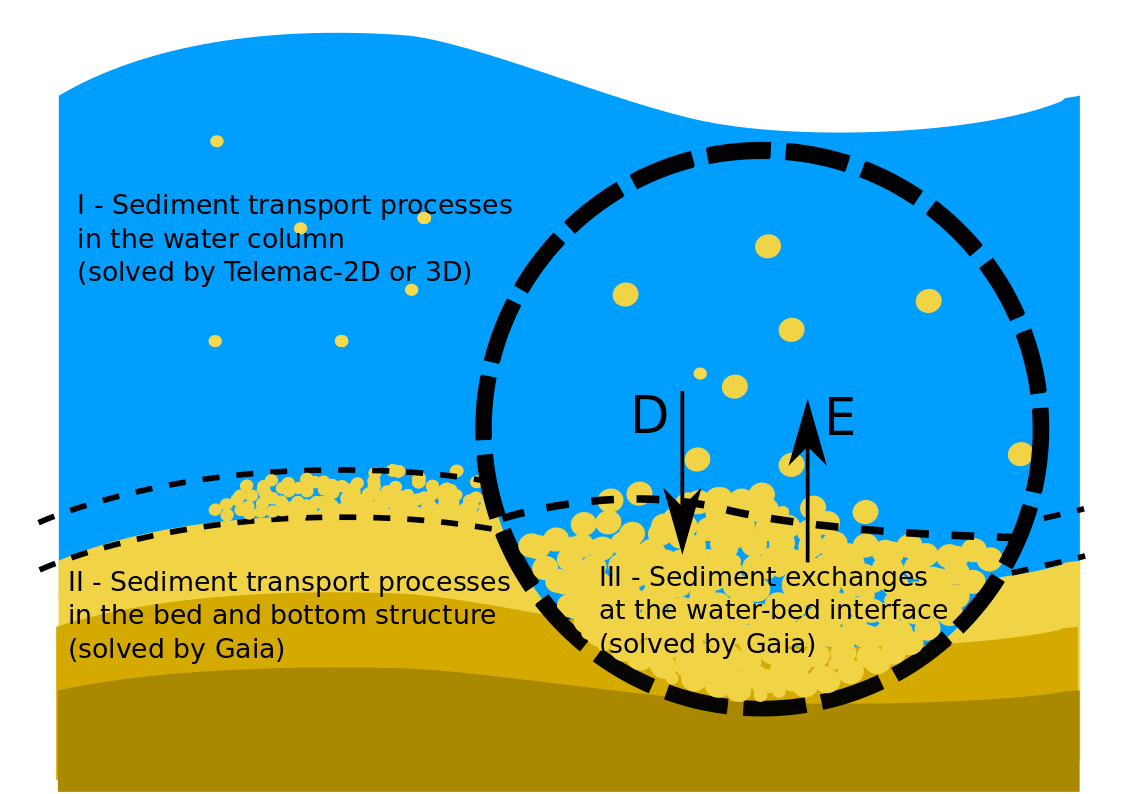
\includegraphics[trim=0 0 0 0, clip,scale=0.22]{./graphics/sediment_transport_processes}
\caption{Sketch summarizing the way in which the sediment transport mechanisms are dealt in \gaia{}. Above, $D$ and $E$ stand for deposition and entrainment fluxes.}
\label{fig:sketch}
\end{figure}


%-------------------------------------------------------------------------------
\subsection{Sediment transport and morphodynamic modelling}
%-------------------------------------------------------------------------------
The prediction of topography changes and sediment discharges can be performed by integrating several modules. It is a {\bf multi--scale problem}, with different physical mechanisms acting according to their space and time response. In summary, the relevant mechanisms that drives morphological changes are:
\begin{itemize}
         \item {\bf hydrodynamics:} with conservative laws of mass and momentum,
         \item {\bf sediment transport:} with predictors for sediment transport capacity,
         \item {\bf bed evolution:} with conservative law for sediment mass.
\end{itemize}
\noindent
Such a modelling system is often referred to as a \emph{morphodynamic model} and is the one adopted in the \telemacsystem{}.

\noindent
From the literature, the main mechanisms of sediment transport are classified as:
\begin{itemize}
\item \textcolor{black}{\bf bedload:} with a variety of closure relationships for sediment transport capacity,
\item \textcolor{black}{\bf suspended load:} with the solution of the advection-diffusion equation (ADE) plus closures for erosion and deposition fluxes, equilibrium concentration,
\item \textcolor{black}{\bf bed evolution:} with the solution of the sediment mass conservation equation or \textit{Exner equation}.
\end{itemize}

\noindent
Different types of sediment can be classified as:
\begin{itemize}
\item \textcolor{black}{\bf non-cohesive:} with equilibrium formulas
\item \textcolor{black}{\bf cohesive:} erosion and deposition laws, consolidation models
\item \textcolor{black}{\bf mixed-size sediments:} accounting for moderately or poorly sorted sediment distribution, sand-gravel and sand-mud mixtures.
\end{itemize}
\noindent


%-------------------------------------------------------------------------------
\subsection{Choice of hydrodynamic models for sediment transport applications}
%-------------------------------------------------------------------------------
The choice of appropriate model equations for flow and sediment transport
will depend upon the scales of interest.

At the scale of ripples, the mechanics of sediment transport could be coupled with the
Reynolds--averaged Navier Stokes equations (NS) to describe the phenomenon.
At large scales, however, the shallow water equations (SWE) are known to
capture quite accurately the salient features --in an average sense-- of
water bodies. The SWE are derived by simplifying the hydrodynamics in the vertical
direction instead of using the full three--dimensional NS or Euler
equations.

As such, the SWE are obtained by assuming a hydrostatic pressure
distribution and a uniform velocity profile across the water layer,
resulting in a two--dimensional problem where the primary variables are the
vertical averages of the horizontal flow velocities and water depth.

This simplification enhances the speed of computations and
facilitates further analytical approaches. In brief, the SWE are often
used to model advection--dominated open channel flows, river and lake
hydrodynamics, floodplain flows, estuarine and coastal circulation as well
as long wave run-up and hydraulic bores, among
other problems of interest within the engineering community~\cite{Vreugdenhil:94}.

%\gaia{} can be coupled with the SWE solver \telemac{2D} and the NS solver \telemac{3D} (see \S\ref{ch:3DBedloadTransport}).

%-------------------------------------------------------------------------------
\subsection{Coupling hydrodynamics to morphodynamics}
%-------------------------------------------------------------------------------
Morphological models can be run fully coupled~\cite{cao02} and decoupled~\cite{vriend87}. In a fully coupled model, sediment
transport and flow occur simultaneously, and thus, their respective
equations are coupled and should be solved simultaneously. Rapid morphological evolution processes due
to hyper-concentrated sediment--laden floods, and debris flow are typical
examples were the fully coupled approach must be employed~\cite{Frac02}.

In contrast, decoupled models are applicable when the typical time scale for river or sea bed adjustment
is much longer than the typical time scale for water flow. The approach used by \gaia{} follows the decoupled treatment, i.e., to alternate between the simulation of flow and bed evolution. This procedure, also known as \textit{asynchronous} solution, considers that the bottom is fixed when the flow variables are computed by the hydrodynamics module.

Hydrodynamic solution is therefore to solve the hydrodynamic continuity and momentum equations on a short time scale.
During this hydrodynamic step the bottom is frozen and the discretized sediment equation is subsequently solved separately.
For the current version of \gaia{}, the decoupled approach is implemented.


\begin{figure}[H]%
\begin{center}
%
\hfil
%
\subfloat[currents only]{
  %
  \vspace{-1cm}
  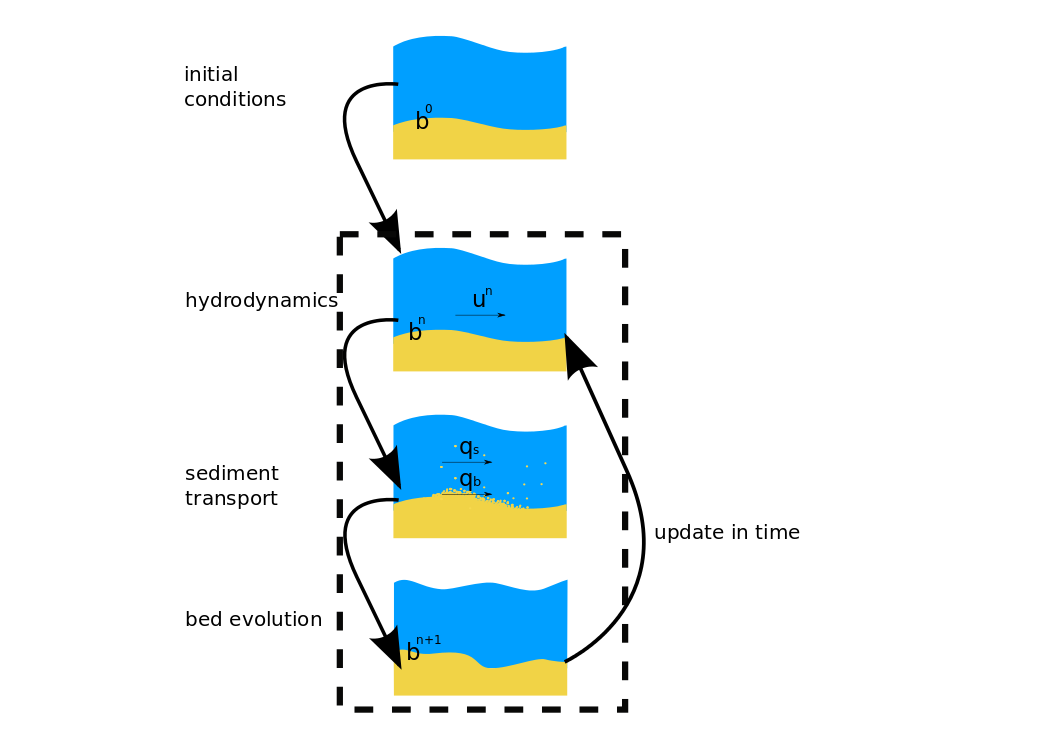
\includegraphics[width=0.55\textwidth]{./graphics/2waycoupling.png}
%
}
%
\hfil
%
\subfloat[currents $+$ waves]{
%
  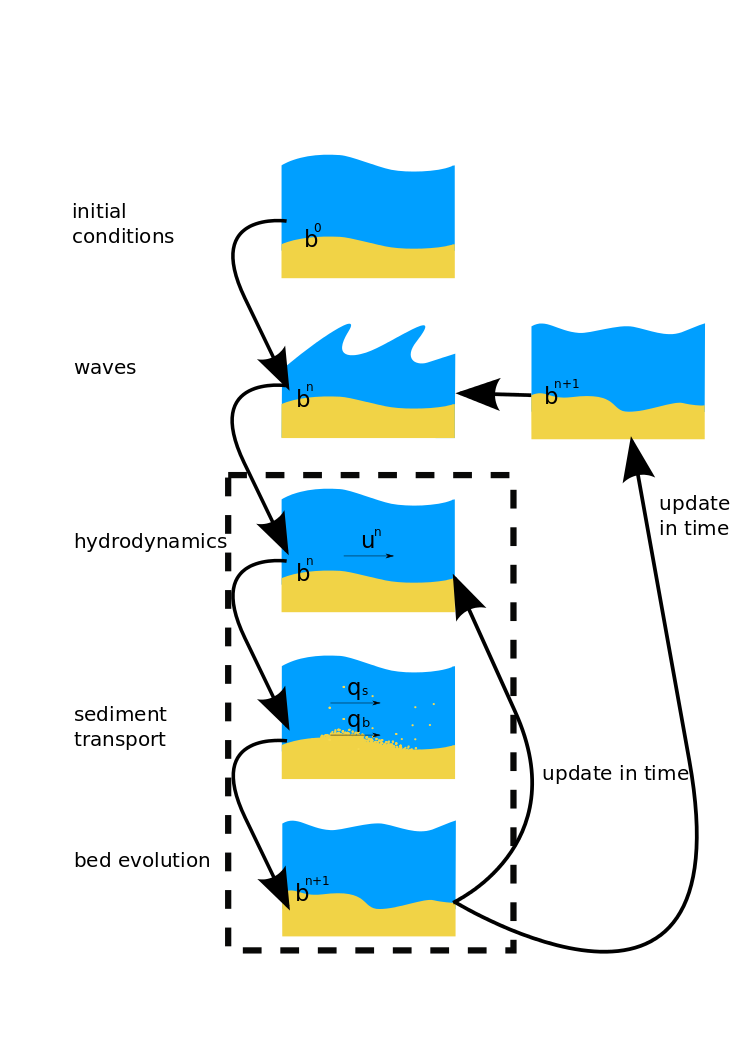
\includegraphics[width=0.4\textwidth]{./graphics/3waycoupling.png}
%
}
%
\hfil
\mbox{}
\end{center}
\caption
[Coupling strategies]
{Schematic coupling strategies for \gaia: (a) coupling morphodynamic and hydrodynamic, current only, (b) coupling morphodynamic and hydrodynamic including the effect of waves.}
\label{fig:CouplingStrategies}
\end{figure}

\pagebreak

%-------------------------------------------------------------------------------
\section{\gaia{}'s structure}
%-------------------------------------------------------------------------------

%...............................................................................
\subsection{Coupling hydrodynamics and morphodynamics}
%...............................................................................
\gaia{} can be internally coupled with the hydrodynamic models \telemac{2D} or \telemac{3D}. In the \telemac{2D} or \telemac{3D} steering files, the following keywords need to be specified:
\begin{itemize}
\item \telkey{COUPLING WITH = 'GAIA'}
\item \telkey{GAIA STEERING FILE = '<name of the gaia steering file>'}
\end{itemize}
For a \textit{hotstart} from a fully developed hydrodynamic, the following information must be included in the \telemac{2D} or \telemac{3D} steering files:
\begin{itemize}
\item \telkey{COMPUTATION CONTINUED} (logical type, set to {\ttfamily = NO} by default)
\end{itemize}
The file name is provided with the keyword \telkey{PREVIOUS COMPUTATION FILE}. Optionally, \telkey{INITIAL TIME SET TO ZERO} (logical type, set to {\ttfamily = NO} by default).

The time step used for morphodynamic computation is the same used for hydrodynamics. It is specified in the \telemac{2D} or \telemac{3D} steering file. For suspended load, the advection-diffusion equation obeys the same Courant number criteria on the time step as the hydrodynamics, and therefore needs to be solved at each time-step. Typically the morphodynamic scale induced by bed load is much smaller, than the hydrodynamic scale. This leads to very small bed level changes in a hydrodynamic time step.

%...............................................................................
\subsection{Equivalence between \gaia{} and \sisyphe{}}
%...............................................................................
Mandatory keywords to be included in \gaia{}'s steering files are:
\begin{itemize}
\item \telkey{TYPE OF SEDIMENT}
\item \telkey{BED LOAD FOR ALL SANDS}
\item \telkey{SUSPENSION FOR ALL SANDS}
\item \telkey{BED-LOAD TRANSPORT FORMULA FOR ALL SANDS}
%\item \telkey{SETTLING VELOCITIES}
%\item \telkey{SHIELDS PARAMETER}
%\item \telkey{SEDIMENT DENSITY}
\end{itemize}
%\pagebreak


\begin{WarningBlock}{Note:}
  Documenting a module such as \gaia{} is a time-consuming, never-ending
  activity that we will try to improve for each new release. Nevertheless,
  the avid reader is referred to the examples folders located at
  \texttt{examples/gaia}, the ``dico'' file, found at
  \texttt{sources/gaia/gaia.dico}, as well as the ``NEWS.txt'' located in
  the root folder of \telemacsystem Git repository, for a glimpse of new
  features, bug fixes and improvements.

  Any remarks, suggestions, corrections, etc. are welcome and can be submitted
  to the \telemacsystem development team through the forum in the Documentation
  category: http://www.opentelemac.org/index.php/kunena/10-documentation.
\end{WarningBlock}

% general introduction to the module

%----------------------------------------------------------------------------------------
%	CHAPTER 2: Sediment Transport Processes in the Water Column
%----------------------------------------------------------------------------------------

%-------------------------------------------------------------------------------
\chapter[Sediment Transport Processes in the Water Column]{Sediment Transport Processes in the Water Column}
\label{chap:SuspendedSedimentTransport}
%-------------------------------------------------------------------------------

Suspended sediment particles being transported by the flow at a given time and maintained in temporary suspension above the bottom by the action of upward-moving turbulent eddies are commonly called \textit{suspended load}. The equation describing mass conservation of suspended sediment is the advection-diffusion equation (ADE), that is valid only for dilute suspensions of particles that are not too coarse (i.e.,~$\leq$ 0.5 mm).

Within this new sediment transport framework, the solution of the ADE, completed with appropriate boundary and initial conditions, is computed by \telemac{2D} or \telemac{3D} for 2D and 3D cases respectively, assuming the suspended sediment as a tracer (passive tracer in 2D and active tracer in 3D). The solution procedure remains almost invisible to the user since the physical parameters are provided by the \gaia{} steering file. Even though, we suggest to readers to refer to the tracer transport chapters of \telemac{2D} and \telemac{3D} user guides for a complete overview of advection-diffusion problems. Two advantages of this procedure are evident: ($i$) to stay up-to-date with the numerical schemes and algorithm developments in the hydrodynamics modules for the solution of the advection terms and ($ii$) for a clearer distinction between sediment transport processes happening in the water column, in the near-bed, and in the bed structure (for example in cases where exchanges with the bottom are not required such as suspended sediment transport over a rigid bed).

The chapter describes the keywords and further user's settings relative to the
suspended sediment transport. The user guides are described without
distinguishing between 2D or 3D where possible. When differences arise between
the 2D and the 3D sediment treatment, a clear distinction is done. No distinction
is done between cohesive and non-cohesive sediments, except when options are
different according to the kind of sediment.

%-------------------------------------------------------------------------------
\section{Advection-diffusion equation for suspended sediment transport}
\label{sec:ADE:suspended}
%-------------------------------------------------------------------------------
%2D suspended transport
In 2D cases, the suspended sediment transport is accounted by solving the two-dimensional advection-diffusion equation, expressed by:
\begin{equation}\label{eq:2DADE}
\frac{\partial hC}{\partial t} + \frac{\partial hUC}{\partial x} + \frac{\partial hVC}{\partial y} =
\frac{\partial}{\partial x}\left(h\epsilon_s\frac{\partial C}{\partial x}\right) +
\frac{\partial}{\partial y}\left(h\epsilon_s\frac{\partial C}{\partial y}\right) + E-D
\end{equation}
where $C=C(x,y,t)$ is the depth-averaged concentration \textcolor{black}{\bf expressed in g/l}, $(U,V)$ are the depth-averaged components of the velocity in the $x$ and $y$ directions, respectively, $\epsilon_s$ is the turbulent diffusivity of the sediment, often related to the eddy viscosity $\epsilon_s=\nu_t/\sigma_c$, with $\sigma_c$ the Schmidt number. In our case, $\sigma_c=1.0$.
$E$ and $D$ are respectively the erosion and deposition fluxes which will be defined in chapter \ref{sec:ExcNCOH} for non-cohesive sediments and in chapter \ref{Chap:Sed:Ex:cohesive} for cohesive sediments.

The value of $\epsilon_s$ can be set through the keyword \telkey{COEFFICIENT FOR
 DIFFUSION OF SUSPENDED SEDIMENTS} (real type value, {\ttfamily = 1.E-6} by
default).

%3D suspended transport
In 3D cases, the suspended sediment transport is accounted by solving the three-dimensional advection-diffusion equation, expressed by:
\begin{equation}\label{eq:3DADE}
\frac{\partial C}{\partial t} + \frac{\partial uC}{\partial x} + \frac{\partial vC}{\partial y} + \frac{\partial wC}{\partial z} -\frac{\partial w_sC}{\partial z} =
\frac{\partial}{\partial x}\left(\epsilon_{sh}\frac{\partial C}{\partial x}\right) +
\frac{\partial}{\partial y}\left(\epsilon_{sh}\frac{\partial C}{\partial y}\right) +
\frac{\partial}{\partial z}\left(\epsilon_{sv}\frac{\partial C}{\partial z}\right) + S
\end{equation}
where $C=C(x,y,z,t)$ is the concentration \textcolor{black}{\bf expressed in g/l}, $(u,v,w)$ are the components of the velocity in the $x$, $y$ and $z$ directions, respectively. $w_s$ is the sediment settling velocity. $(\epsilon_{sh}, \epsilon_{sv})$ are the diffusion coefficients in the horizontal and vertical directions, respectively.
$S$ is sources or sinks term.
$z$ ranges from $-H(x,y,t)$, the lowest limit where the water is undisturbed,
 to $WSE(x,y,t)$, the water surface elevation.
\begin{equation*}\label{eq:at_mH}
At ~~~ z=-H(x,y,t)~, w_sC + \epsilon_{sv}\frac{\partial C}{\partial z} = D-E
\end{equation*}
where $D$, $E$ are the deposition and erosion fluxes respectively.
They will be defined and detailed in chapter \ref{sec:ExcNCOH} for non cohesive
sediments and in chapter \ref{Chap:Sed:Ex:cohesive} for cohesive sediments.

The value of $\epsilon_{sh}$ can be set through the keyword \telkey{COEFFICIENT FOR
 HORIZONTAL DIFFUSION OF SUSPENDED SEDIMENTS} (real type list, {\ttfamily = 1.E-6}
by default). The value for $\epsilon_{sv}$ can be set through the keyword
\telkey{COEFFICIENT FOR VERTICAL DIFFUSION OF SUSPENDED SEDIMENTS}
(real type list, {\ttfamily = 1.E-6} by default)

It is worth to notice that concentration must always be expressed in g/l
(e.g. for the initial concentration of sediments and so on) since some parts
of the equations like source terms
in 2D are coded considering g/l as unit. If user wishes to refer to volume
concentration he needs to do this in a post-processing step. We recall that
$C_v=C_m/\rho_s$ where $C_m$ is tha mass concentration (g/l) and $\rho_s$ is the
sediment density (kg/m$^3$) while $C_v$ is the
volume concentration (/), which express the ratio between the solid volume and
the total volume (solid volume + water volume). The mass concentration express
the ratio between the mass of suspended sediment (dry weight of solids) and the
total volume.

The suspended load can be activated through the keyword \telkey{SUSPENSION FOR ALL
SANDS} (logical type , {\ttfamily = NO} by default) in case of non-cohesive
sediments while is automatically activated for cohesive sediments.

%...............................................................................
\section{Initial conditions for suspended sediment transport}
%...............................................................................
The initial condition value of the concentration can be specified through the keyword \telkey{INITIAL SUSPENDED SEDIMENTS CONCENTRATION VALUES} (real type list, {\ttfamily = 0.0} by default), following the order given in \telkey{CLASSES TYPE OF SEDIMENT}.
These values must be \textcolor{black}{\bf expressed in g/l}. In 2D, this keyword is not considered on boundary nodes if \texttt{EQUILIBRIUM INFLOW CONCENTRATION = YES}.\\

\begin{lstlisting}[frame=trBL]
INITIAL SUSPENDED SEDIMENTS CONCENTRATION VALUES :0.D0;1.D0;...
\end{lstlisting}

\section{Boundary conditions for suspended sediment transport}

The specification of boundary conditions is done in a boundary condition file, usually named with extension \texttt{*.cli}. The reader is referred to \S\ref{sec:flags} for the definition of the different flags used in the boundary condition file.

\subsection{Wall boundary conditions}
At banks and islands, the no-flux boundary condition is imposed: the suspended load concentration gradients are set to zero.
\begin{equation}
\label{eq:BC-noflux}
\epsilon_s\frac{\partial C}{\partial n}=\epsilon_s \Grad C \cdot \vec{n}=0
\end{equation}
For this case, the flag \texttt{LIEBOR} is set \texttt{= 2} as shown in the example below:

\begin{lstlisting}[frame=trBL]
2 2 2 0.0 0.0 0.0 0.0 (*@\color{PantoneRed}2@*) 0.0 0.0 0.0 565 1
\end{lstlisting}

\subsection{Inflow boundary conditions}
Several ways to impose the concentration at inflow boundary conditions are proposed in \gaia. For this case, the flag \texttt{LICBOR} is set \texttt{= 5}, with the following options for the concentration values:
\begin{itemize}
\item Specified in the column \texttt{CBOR}. In the example below, a concentration value {\ttfamily = 1.0} g/l is provided:
\begin{lstlisting}[frame=trBL]
4 5 5 0.0 0.0 0.0 0.0 (*@\color{PantoneRed}5@*) (*@\color{PantoneRed}1.0@*) 0.0 0.0 565 1
\end{lstlisting}
\item Specified by the concentration values at the boundary through the keyword \telkey{PRESCRIBED SUSPENDED SEDIMENTS CONCENTRATION VALUES} (real type list of size equal to the number of boundaries $\times$ the number of sediment classes), expressed in g/l:
\begin{lstlisting}[frame=trBL]
4 5 5 0.0 0.0 0.0 0.0 (*@\color{PantoneRed}5@*) 0.0 0.0 0.0 565 1
\end{lstlisting}
\begin{lstlisting}[frame=trBL]
  PRESCRIBED SUSPENDED SEDIMENTS CONCENTRATION VALUES =
  0.0; 0.0; 1.0; ...
\end{lstlisting}
The order is the following: boundary 1 (class 1, class2, etc.), then boundary 2, etc.
\item Computed by \gaia{} in 2D cases through the keyword \telkey{EQUILIBRIUM INFLOW CONCENTRATION} (logical type variable, {\ttfamily = NO} by default).
For non-choesive sediments, the equilibrium inflow concentration will be computed also according to the choice of the formula of equilibrium near-bed concentration (\telkey{SUSPENSION TRANSPORT FORMULA FOR ALL SANDS = 1} by default).

\begin{lstlisting}[frame=trBL]
4 5 5 0.0 0.0 0.0 0.0 (*@\color{PantoneRed}5@*) 0.0 0.0 0.0 565 1
\end{lstlisting}
\begin{lstlisting}[frame=trBL]
EQUILIBRIUM INFLOW CONCENTRATION = YES
SUSPENSION TRANSPORT FORMULA FOR ALL SANDS = 1
\end{lstlisting}
\item Time-varying concentration values (in g/l) must be provided in an external \texttt{ASCII} file. In this case the keyword \telkey{LIQUID BOUNDARIES FILE} has to be used in the hydrodynamic steering file of \telemac{2D} or \telemac{3D} according to the case. Suspended sediment concentrations are treated like tracers, the reader is thus referred to the user manual of modules \telemac{2D} or \telemac{3D}.
If tracers and sediments are declared at the same time, sediments will be allocated after tracers. For example if we have 3 tracers and 2 suspended sediments, the first sediments will be the fourth tracer.
\begin{lstlisting}[frame=trBL]
4 5 5 0.0 0.0 0.0 0.0 (*@\color{PantoneRed}5@*) 0.0 0.0 0.0 565 1
\end{lstlisting}
\begin{lstlisting}[frame=trBL]
LIQUID BOUNDARIES FILE = '<file name>'
\end{lstlisting}
\item Vertical profile provided in 3D cases through the keyword \telkey{VERTICAL PROFILES OF SUSPENDED SEDIMENTS}, which can be equal to:
\begin{itemize}
\item 0 if the profile is programmed by users,
\item 1 if constant profile,
\item 2 if Rouse profile,
\item 3 if normalised Rouse profile and assigned concentration,
\item 4 if modified Rouse profile with molecular viscosity.
\end{itemize}
\end{itemize}

According to the hydrodynamic forcing, the use of the keyword \telkey{EQUILIBRIUM INFLOW CONCENTRATION} can be used to prevent the excessive erosion and deposition on the inflow boundary (for 2D cases).

Stability issues at inflow boundaries can be solved by activating the keyword \telkey{TREATMENT OF FLUXES AT THE BOUNDARIES} (integer type variable, {\ttfamily = 1}, default option) in the steering file of \telemac{2D} or \telemac{3D}. The choice {\ttfamily = 1} can be activated when prescribed values are provided. The choice {\ttfamily = 2} is used when fluxes are imposed, allowing a correct mass balance.
The latter is strongly reccomended for mass-conservation reasons.

\subsection{Outflow boundary conditions}
At the outflow boundary, the suspended load concentration gradient in the flow direction is set to zero. For this case, the flag \texttt{LICBOR} is set \texttt{= 4} as shown in the example below:

\begin{lstlisting}[frame=trBL]
5 4 4 0.0 0.0 0.0 0.0 (*@\color{PantoneRed}4@*) 0.0 0.0 0.0 565 1
\end{lstlisting}

%...............................................................................
%\subsection{Diffusion and dispersion} -> what about this part now?
%%...............................................................................
%The diffusion term in the ADE for the depth-averaged suspended concentration is taken into account with the keyword \telkey{ DIFFUSION} (logical type, set {\ttfamily = YES} by default). The values of the diffusion coefficients can be specified with the keyword \telkey{ OPTION FOR THE DISPERSION} (integer type, set {\ttfamily = 1} by default), with the following options:
%\begin{itemize}
%\item {\ttfamily = 1}: values of the longitudinal and transversal dispersion coefficients are provided with the keywords \texttt{DISPERSION ALONG THE FLOW} and \texttt{DISPERSION ACROSS THE FLOW}, respectively:
%\begin{itemize}
%\item \telkey{DISPERSION ALONG THE FLOW} (real type, set {\ttfamily = $1.0 \times 10^{-2}$ m$^2/$s} by default)
%\item \telkey{DISPERSION ACROSS THE FLOW} (real type, set {\ttfamily = $1.0 \times 10^{-2}$ m$^2/$s} by default)
%\end{itemize}
%
%\item {\ttfamily = 2}: values of the longitudinal and transversal dispersion coefficients are computed with the Elder model $T_l=\alpha_l u_* h$ and $T_t=\alpha_t u_* h$, where the coefficients $\alpha_l$ and $\alpha_t$ can be provided with the keywords \texttt{DISPERSION ALONG THE FLOW} and \texttt{DISPERSION ACROSS THE FLOW}.
%\item {\ttfamily = 3}: values of the dispersion coefficients are provided by the hydrodynamics module (e.g. \telemac{2D})
%\end{itemize}

%...............................................................................
\section{Numerical treatment of the advection terms}
%...............................................................................
The choice for the scheme for the treatment of the advection terms can be done with the keyword \texttt{SCHEME FOR ADVECTION OF SUSPENDED SEDIMENTS} (integer type, set {\ttfamily = 5} by default):
\begin{lstlisting}[frame=trBL]
1="CHARACTERISTICS"
2="SUPG"
4="N SCHEME"
5="PSI SCHEME"
13="EDGE-BASED N SCHEME"
14="EDGE-BASED N SCHEME"
15="ERIA SCHEME" (only for 2D)
\end{lstlisting}

The keyword \texttt{SCHEME OPTION FOR ADVECTION OF SUSPENDED SEDIMENTS} can be used to choose futher options for some of the advection schemes. In particular, if characteristics are used (i.e. \texttt{SCHEME FOR ADVECTION OF SUSPENDED SEDIMENTS = 1}), the following options are possible :
\begin{itemize}
\item \texttt{1}: strong form;
\item \texttt{2}: weak form.
\end{itemize}
If advection is solved by the N or PSI scheme (i.e. \texttt{SCHEME FOR ADVECTION OF SUSPENDED SEDIMENTS = 4 or 5}), options are:
\begin{itemize}
\item \texttt{1}: explicit scheme;
\item \texttt{2}: first order predictor-corrector scheme;
\item \texttt{3}: second order predictor-corrector scheme;
\item \texttt{4}: local semi-implicit scheme.
\end{itemize}
The keyword \texttt{SCHEME OPTION FOR ADVECTION OF SUSPENDED SEDIMENTS} is not
useful when using \texttt{SCHEME FOR ADVECTION OF SUSPENDED SEDIMENTS}
{\ttfamily = 2,13,14,15} since these schemes haven't further options.

To have more details about these keywords, readers can refer to the \telemac{2D} or \telemac{3D} user guide (cf. chapters about tracer advection). In fact, the advection scheme used by sediments is exactly the same used by tracers, implemented in hydrodynamics modules. Keywords \texttt{SCHEME FOR ADVECTION OF SUSPENDED SEDIMENTS} and \texttt{SCHEME OPTION FOR ADVECTION OF SUSPENDED SEDIMENTS} have been added from V8P2 in \gaia{} in order to have proper steering files.

\begin{WarningBlock}{Note:}
  For completely wet cases it is recommended to use the schemes {\ttfamily 5} or
 {\ttfamily 14} for a good compromise between accuracy and computational time
 (i.e. first order schemes in time and low CPU time). If more accuracy is needed
 then
 it is suggested to use the scheme {\ttfamily 4} with option {\ttfamily 3}:
 second order scheme but higher CPU time.
 When tidal flats are present, it is recommended to use scheme {\ttfamily 14}
 for a good compromise between accuracy and computational time. If more accuracy
 is needed it is suggested to use scheme {\ttfamily 4} with option {\ttfamily 4}
 or scheme {\ttfamily 15}.
 For 2D simulations is also suggested to activate the keyword \telkey{CONTINUITY
 CORRECTION = YES} in the steering file of \telemac{2D}.
\end{WarningBlock}

A brief description of the numerical schemes implemented in \gaia{} is given below:
\begin{itemize}
\item \textbf{Method of characteristics} (\texttt{1})
\begin{itemize}
\item Unconditionally stable and monotonous
\item Diffusive for small time steps
\item Not conservative
\end{itemize}
\item \textbf{Method Streamline Upwind Petrov Galerkin SUPG} (\texttt{2})
\begin{itemize}
\item Based on the Courant number criteria
\item Less diffusive for small time steps,
\item Not conservative
\end{itemize}
\item \textbf{N-scheme (similar to finite volumes)} (\texttt{4})
\begin{itemize}
\item Conservative: solves the continuity equation under its conservative form
\item Recommended for correction on convection velocity
\item Courant number limitation (sub-iterations to reduce time step)
\end{itemize}
\item \textbf{Edge-based N-scheme NERD} (\texttt{13, 14})
\begin{itemize}
\item Same as \texttt{4} but adapted to tidal flats
\item Based on positive-depth algorithm
\end{itemize}
\item \textbf{Distributive schemes PSI} (\texttt{5})
\begin{itemize}
\item Fluxes corrected according to the tracer value: relaxation of Courant number criteria, less diffusive than
schemes \texttt{4, 14} (since second order in space) but larger CPU time
\item Should not be applied for tidal flats
\end{itemize}
\item \textbf{Eria scheme} (\texttt{15})
\begin{itemize}
\item Works for tidal flats
\item Less diffusive than \texttt{14}
\end{itemize}
\end{itemize}
For further information about these schemes, refer to \telemac{2D} user manual.

%...............................................................................
\section{Numerical treatment of the diffusion terms}
%...............................................................................
\subsection{Bidimensional case}
The keyword \telkey{OPTION FOR THE DIFFUSION OF TRACER} (integer type, set {\ttfamily = 1} by default) allows to choose the treatment of the diffusion terms in the advection-diffusion equation \ref{eq:2DADE} for the depth-averaged suspended concentration:
\begin{itemize}
\item \texttt{= 1}: the diffusion term is solved in the form $\nabla\cdot(\varepsilon_s\nabla C)$
\item \texttt{= 2}: the diffusion term is solved in the form $\frac{1}{h}\nabla\cdot(h\varepsilon_s\nabla C)$
\end{itemize}
This keyword must be activated in the steering file of \telemac{2D}; user can refer to the corresponding user manual for further details.
The scheme used to solve the diffusion term is a completely implicit scheme.
\subsection{Tridimensional case}
The keyword \telkey{SCHEME FOR DIFFUSION OF SUSPENDED SEDIMENTS IN 3D} (integer type, set {\ttfamily = 1} by default) allows to choose the treatment of the diffusion terms. Choices are:
\begin{itemize}
\item \texttt{= 0}: the diffusion terms are not taken into account
\item \texttt{= 1}: the diffusion terms are solved by a scheme with a variable implicitation coefficient
\end{itemize}
The implicitation coefficient used for option {\ttfamily = 1} can be set through
the keyword \telkey{IMPLICITATION FOR DIFFUSION} (real type, set {\ttfamily = 1.}
by default). This last keyword must be activated in the steering file of
\telemac{3D}.
% copy the keyword in GAIA?
\subsection{Solution of the linear system}
As for the tracers in \telemac{2D} and in \telemac{3D}, the following
keywords can be used to set the numerical parameters related to the solution
 of the linear system:
\begin{itemize}
\item \telkey{SOLVER FOR DIFFUSION OF SUSPENSION} (integer type list, set
{\ttfamily = 1} by default). For each suspended sediments, the following
options are possible:
%from T3D user doc
 \begin{itemize}
\item 1: conjugate gradient method (when the matrix of the system to solve
is symmetric),

\item 2: conjugate residual method,

\item 3: conjugate gradient on a normal equation method,

\item 4: minimum error method,

\item 5: square conjugate gradient method,

\item 6: CGSTAB (stabilized conjugate gradient) method,

\item 7: GMRES (Generalised Minimum RESidual) method,

\item 8: direct solver (YSMP, solver of the Yale university),
does not work in parallel mode.
 \end{itemize}
\item \telkey{SOLVER OPTION FOR DIFFUSION OF SUSPENSION} (integer type, set
 {\ttfamily = 5} by default). This option is useful only for the GMRES solver
and states the dimension of the Krylov space used by the solver.
\item \telkey{MAXIMUM NUMBER OF ITERATIONS FOR SOLVER FOR SUSPENSION} (integer
type list, set {\ttfamily = 60} by default). It states the maximum number of
iterations used to solve the linear system at every time step.
\item \telkey{ACCURACY FOR DIFFUSION OF SUSPENSION} (real type, set to {\ttfamily
 = 1.E-8}) by default.
\item \telkey{PRECONDITIONING FOR DIFFUSION OF SUSPENSION} (integer type list, set
{\ttfamily = 2} by default). The solution of the linear system can be facilitate
by the preconditioning of matrices. For each solver used for suspended sediments,
the following options are available:
%from T3D user doc
\begin{itemize}
\item 0:  no preconditioning,

\item 2:  diagonal preconditioning,

\item 3:  diagonal preconditioning with the condensed matrix,

\item 5:  diagonal preconditioning with absolute values,

\item 7:  Crout preconditioning per elementCrout (downgraded in parallel),

\item 11: Gauss-Seidel preconditioning per element (downgraded in parallel),

\item 13: preconditioning matrix is provided by the user,

\item 14: cumulated diagonal preconditioning and Crout preconditioning per
element,

\item 17:  preconditioning through direct solution along each vertical
direction,

\item 21:  cumulated diagonal preconditioning with the condensed matrix and
Crout preconditioning per element,

\item 34:  cumulated diagonal preconditioning with direct solution along each
vertical direction.
\end{itemize}
Options {\ttfamily = 17,21,34} are only for 3D simulations.
\end{itemize}
Information about the solvers are printed in the listing printout of a
run. If the maximum number of iterations is reached, this number can be increased
but it is suggested to not exceed high values (like 150/200). It is rather
recommended to reduce the time step in order to improve the convergence.

The user is invited to look to the \telemac{2D} and \telemac{3D} user
documentation for more details about these numerical settings for solvers.
%...............................................................................
\section{Correction of the convection velocity (in 2D)}
%...............................................................................
As most of the sediment transport processes occur near the bed, it often exhibits an over-estimation of suspended sand transport.
A correction method accounting for the vertical velocity and concentration profiles is therefore proposed {\bf for 2D simulations}. A straightforward treatment of the advection terms would imply the
definition of an advection velocity and replacement of the depth-averaged
velocity $U$ along the $x-$axis in Eq.~(\ref{eq:2DADE}) by:
\begin{equation*}
U_{conv} = \overline{UC}/C.
\end{equation*}
A correction factor is introduced in \gaia, defined by:
\begin{equation*}
F_{conv} =\frac{U_{conv}}{U}.
\end{equation*}
A similar treatment is done for the depth-averaged velocity $V$ along the $y-$axis. For further details, see~\cite{Huybrechts}.
The convection velocity should be smaller than the mean flow velocity ($F_{conv} \leq 1$) since sediment concentrations are mostly transported in the lower part of the water column where velocities are smaller. We further
assume an exponential concentration profile which is a reasonable
approximation of the Rouse profile, and a logarithmic velocity profile, in
order to establish the following analytical expression for $F_{conv}$:
\begin{equation*}
F_{conv} =-\frac{I_2 - \ln\left(\frac{B}{30}\right) I_1}{I_1 \ln\left(
\frac{eB}{30}\right)},
\end{equation*}
with $B=k_s/h = Z_{ref}/h$ and
\begin{equation*}
I_1 =\int_B^1\left(\frac{(1-u)}{u}\right)^R du,\quad I_2 = \int_B^1 \ln u \left(\frac{(1-u)}{u} \right)^R du.
\end{equation*}

The keyword \texttt{CORRECTION ON CONVECTION VELOCITY = YES} (logical type, set {\ttfamily = NO} by default) modifies the depth-averaged convection velocity to account for the vertical gradients of velocities and concentration.

%...............................................................................
\section{Settling lag correction (for non-cohesive sediments, in 2D)}
%...............................................................................
Sediment transport exhibits temporal lags with flow due to flow and sediment velocity difference and bed development~\cite{wu2007computational, Miles96}. A scaling factor that accounts for both the settling velocity and the lag time is therefore required for the saturation concentration profile to adjust to changes in the flow {\bf in case of non-cohesive sediments}.
The keyword \telkey{SETTLING LAG} (logical type, set to \texttt{NON} by default) allows to compute the bed exchange factor beta based on Miles~\cite{Miles96} {\bf in 2D simulations}. This keyword must be used with the Nikuradse friction law, prescribed in the \telemac{2D} steering file as \telkey{LAW OF BOTTOM FRICTION = 5}.

%...............................................................................
\section{Flocculation models (for cohesive sediments, in 3D)}
%...............................................................................
If the keyword \telkey{FLOCCULATION} (logical type variable, set to {\ttfamily = NO} by default) is activated, flocculation processes can be accounted in \gaia only for coupling with \telemac{3D}. The choice of the available models can be done through the keyword \telkey{FLOCCULATION FORMULA} {\ttfamily = 1} by default).
\subsection{Van Leussen's model (1994)}
The fall velocity is modified as follows:
\begin{equation*}
w_{s}^{modif} = w_s \times \frac{1+A \times G}{1 + B\times G^{2}},
\end{equation*}
where $A$ [s] and $B$ [s] are the Van Leussen relative coefficients to floc formation and destruction respectively, and $G$ [s$^{-1}$] represents the shear rate, defined as a function of the velocity gradient $\partial U/\partial z$~\cite{Camp1943}:
\begin{equation*}
G = \sqrt{\frac{\epsilon}{\nu}}=\sqrt{\frac{\frac{\tau}{\rho}\frac{\partial U}{\partial z}}{\nu}}=\sqrt{\frac{u^{*2}\frac{\partial U}{\partial z}}{\nu}}
\end{equation*}

The coefficient for floc formation $A$ can be set via the keyword \telkey{FLOCCULATION COEFFICIENT} (real value, equal to 0.3 s$^{-1}$ by default). The coefficient for floc destruction $B$ can be set via the keyword \telkey{COEFFICIENT RELATIVE TO FLOC DESTRUCTION} (real value, equal to 0.09 s$^{-2}$ by default).
This formula is activated as follows: \telkey{FLOCCULATION FORMULA = 1}.
\subsection{Soulsby et al's model (2013)}
This model computes the fall velocity of mud flocs based on Soulsby \texttt{et al.}~\cite{SOULSBY20131}, derived from Manning's floc database.
This formula is activated as follows: \telkey{FLOCCULATION FORMULA = 2}.
\subsection{User defined model}
By using the keyword \telkey{FLOCCULATION FORMULA = 0}, a user's defined flocculation model can be implemented by the user. To this goal, subroutines \texttt{user\_compute\_settling\_vel.f} is available in the folder \texttt{sources/telemac3d}.

%...............................................................................
\section{Hindered formulations (for cohesive sediments, in 3D)}
%...............................................................................
If the keyword \telkey{HINDERED SETTLING} (logical type variable, set to {\ttfamily = NO} by default) is activated, the hindered formulation is used to compute the settling velocities in \gaia only for coupling with \telemac{3D}. The choice of the available formulations can be done through the keyword \telkey{HINDERED SETTLING FORMULA} {\ttfamily = 1} by default). \\
The different formulations are:
\begin{itemize}
\item User defined formula, set by \telkey{HINDERED SETTLING FORMULA} {\ttfamily = 0};
\item Whitehouse et al. (2000), set by \telkey{HINDERED SETTLING FORMULA} {\ttfamily = 1};
\item Winterwerp (1999), set by \telkey{HINDERED SETTLING FORMULA} {\ttfamily = 2}.
\end{itemize}
To use the user's defined formula, the subroutine \texttt{user\_hindering\_formula.f} needs to be modified. The subroutine is available in the folder \texttt{sources/telemac3d}.



%----------------------------------------------------------------------------------------
%	CHAPTER 3: Sediment Transport Processes in the Bed and Stratigraphy
%----------------------------------------------------------------------------------------

%-------------------------------------------------------------------------------
\chapter[Sediment Transport Processes in the Bed and Stratigraphy]{Sediment Transport Processes in the Bed and Stratigraphy}
%-------------------------------------------------------------------------------

\pagebreak
%-------------------------------------------------------------------------------
\section[Bedload sediment transport]{Bedload Transport}\label{sec:BedloadTransport}
%-------------------------------------------------------------------------------
Sediment particles which are transported in direct contact with the bottom or next to the bed without being affected by the fluid turbulence are commonly called \textit{bedload}. \textbf{In contrast to \textsc{Sisyphe}, in \textsc{Gaia} bedload fluxes are computed in terms of (dry) mass transport rate per unit width, without pores.} The numerical computation of sediment fluxes in terms of dry mass minimizes roundoff error, particularly for the mass transfer algorithms used for the bed layer model.

%-------------------------------------------------------------------------------
\subsection{Preliminaries}
%-------------------------------------------------------------------------------
The classical form of the conservative law equation for sediment mass (or Exner equation) accounts for the vector of volumetric transport rate per unit width without pores $\mathbf Q_b$, expressed in (m$^2/$s), with components $Q_{b_x}, Q_{b_y}$ in the $x$ and $y$ direction respectively. The bedload transport vector can be decomposed into $x-$ and $y-$direction components as:
\begin{align}
\mathbf Q_b = (Q_{b_x}, Q_{b_y}) = (Q_b \cos\alpha, Q_b \sin\alpha).
\label{eq:bedloadtransportvector}
\end{align}
Above, $Q_b$ is the bedload transport rate per unit width, computed as a function of the equilibrium sediment load closure (or sediment transport capacity) and $\alpha$ is the angle between the sediment transport vector and the downstream direction ($x-$axis). The deviation of the bed load direction from the flow direction is mainly influenced by the bed slope and the presence of secondary flows~\cite{Talmon95}, see Section~\ref{sec:corrections}.

As presented and discussed in \S~\ref{sec:bedevol}, \gaia{} solves the Exner equation as a function of the mass transport flux rate and not in terms of volumetric transport rate, as follows:
\begin{equation}
\mathbf Q_{mb}=\rho_s \mathbf Q_b,
\end{equation}
where $\mathbf Q_{mb}$ is the vector of mass transport rate per unit width without pores (kg/(m~s)), with $\rho_s$ the sediment density.

%The equation is obtained writing the conservative law equation for sediment and integrating along the vertical, keeping density in the equation:
%\begin{align}
%(1-\lambda)\frac{\partial \left(\rho z_b\right)}{\partial t} + \nabla\cdot \left(\mathbf Q_{mb} z_b\right) = 0
%\label{eq:Exner_mass}
%\end{align}
%\textcolor{blue}{where $\mathbf Q_{mb}=\rho \mathbf Q_b$ is the vector of mass transport rate per unit width without pores (kg/(m~s)).}

%...............................................................................
\subsection{Steering file setup for bedload transport}
%...............................................................................
For non-cohesive sediments, the bedload sediment transport can be set with the keyword \telkey{BED LOAD FOR ALL SANDS = YES} (logical type variable, set to {\ttfamily = NO} by default). This keyword explicitly stated that all non-cohesive sediments considered in the computation will be transported by the bedload sediment transport mechanism.

The dimensionless current-induced sediment transport rate $\Phi_b$ is expressed by:
\begin{align}
\Phi_b = \frac{Q_b}{\sqrt{g(s-1)d^3}},
\label{eq:Phis}
\end{align}
with $s=\rho_s/\rho$ the relative density ($-$); $\rho_s$ the sediment density (kg$/$m$^3$), with corresponding keyword \telkey{CLASSES SEDIMENT DENSITY} and default value equal to $2650$ kg/m$^3$; $\rho$ the water density (kg$/$m$^3$); $d$ the sand grain diameter ($=d_{50}$ for uniform sediment distribution (m)) and $g$ the gravity acceleration constant (m$/$s$^2$). The keyword \telkey{CLASSES SEDIMENT DIAMETERS} allows the user to introduce the mean sand grain diameter per class.

Different choices of $\Phi_b$ can be selected with the keyword \telkey{BED-LOAD TRANSPORT FORMULA FOR ALL SANDS} (integer type variable, set to {\ttfamily = 1} by default corresponding to the Meyer-Peter and M\"uller formula). This keyword explicitly stated that all non-cohesive sediments considered in the computation will account for the same sediment transport capacity formula. %\textcolor{blue}{As the keyword explicitly says, it can be used exclusively for non cohesive sediments and in case of non uniform sediment transport, user can choose only one formula that will be applied to all sediments. If there are non cohesive sediments, the transport formula is automatically chosen by \gaia{}. EXPLAIN BETTER?}

%...............................................................................
\subsubsection{Bedload transport formulas}
%...............................................................................
Bedload transport formulas are generally computed as function of the Shields number $\theta$:
\begin{align}
\theta=\frac{\mu\tau_b}{(\rho_s-\rho)gd},
\label{eq:shieldsp}
\end{align}
with $\tau_b$ the bottom shear stress [Pa] and $\mu$ the correction factor for skin friction (discussed later in Section~\ref{sec:skin}).

Keyword \telkey{BED-LOAD TRANSPORT FORMULA FOR ALL SANDS} (integer type variable, set to {\ttfamily = 1} by default) can be used to set a bedload transport formula.
Available formulas in \gaia{} for bedload transport are:
\begin{lstlisting}[frame=trBL]
1 : MEYER-PETER and MUELLER
2 : EINSTEIN-BROWN
3 : ENGELUND-HANSEN + CHOLLET ET CUNGE (total sediment transport)
10: WILCOCK AND CROWE
30: ENGELUND-HANSEN (total sediment transport)
7 : VAN RIJN
\end{lstlisting}
For example, the keyword \telkey{BED-LOAD TRANSPORT FORMULA FOR ALL SANDS = 7} sets the van Rijn formula. Please note that bedload transport formulas \telkey{3} and \telkey{30} account for the total sediment transport.

%...............................................................................
\subsubsection{Available bedload transport formulas}
%...............................................................................
\subsubsection{Meyer-Peter and M\"uller}
\begin{itemize}
\item \telkey{BED-LOAD TRANSPORT FORMULA FOR ALL SANDS = 1}
\item Classical, wide application range $d=d_{50} = [0.4-29]$mm, based on grain mouvement threshold concept. The dimensionless current-induced sediment transport rate is given by:
\begin{equation*}
\Phi_b=\left\{\begin{array}{ll}
0 & \text{if}\,\theta<\theta_{cr}\\
\alpha_{mpm}(\theta-\theta_{cr})^{3/2} & \text{otherwise}
\end{array}
\right.
\end{equation*}
with $\alpha_{mpm}$ a coefficient and $\theta_{cr}$ the critical Shields parameter (keyword \telkey{CLASSES SHIELDS PARAMETERS})

   \begin{WarningBlock}{Note:}
  To be consistent with the classical Meyer-Peter and M\"uller formula, the value of the critical Shields parameter $\theta_{cr}$ must be explicitly set equal to 0.047 in the steering file (\telkey{CLASSES SHIELDS PARAMETERS = 0.047}).
\end{WarningBlock}

\item For calibration purposes, the coefficient $\alpha_{mpm}$ can be modified in the steering file by the keyword \telkey{MPM COEFFICIENT} (real type variable, {\ttfamily = 8} by default).

  \begin{WarningBlock}{Note:}
  A value of \telkey{MPM COEFFICIENT = 8} was proposed for the original MPM formula~\cite{GarciaBook2006} with $\theta_{cr}=0.0470$, while \telkey{MPM COEFFICIENT = 3.97} is equivalent to the modified Meyer-Peter and M\"uller formula proposed by Wong and Parker~\cite{WongParker06}, with $\theta_{cr}=0.0495$.
  \end{WarningBlock}



\item Fortran subroutine {\ttfamily bedload\_meyer.f}.

\end{itemize}

\subsubsection{Einstein-Brown}
\begin{itemize}
\item \telkey{BED-LOAD TRANSPORT FORMULA FOR ALL SANDS = 2}
\item Based on the energy concept (no threshold), valid for gravel and large shear
stresses (application range $d=d_{50} = [0.25-32]$mm). The dimensionless current-induced sediment transport rate is given by:
\begin{equation*}
\Phi_b = F(D_*)f(\theta),
\end{equation*}
with
\begin{equation*}\label{eq:EinsteinFDs}
F(D_*) = \left(\frac{2}{3} +\frac{36}{D_*}\right)^{0.5} - \left( \frac{36}{D_*}\right)^{0.5},
\end{equation*}
and
\begin{equation*}
f(\theta)=\left\{\begin{array}{ll}
2.15\exp(-0.391/\theta) & \quad\text{if}\,\,\theta \leq 0.2 \\
40\,\theta^{3}          & \quad\text{otherwise}
\end{array}
\right.
\end{equation*}
where $D_*=d[(\rho_s/\rho-1)g/\nu^2]^{1/3}$ is the non-dimensional diameter,
with $\rho_s$ the sediment density (keyword \telkey{CLASSES SEDIMENT DENSITY}, equal to
2650~kg/m$^3$ by default),
$\rho$ the water density (keyword \telkey{WATER DENSITY}, equal to 1000~kg/m$^3$ by default in
\telemac{2D} or \telkey{AVERAGE WATER DENSITY}, equal to 1025~kg/m$^3$ by default in
\telemac{3D}),
$\nu$ the water viscosity (keyword \telkey{WATER VISCOSITY}, equal to $10^{-6}$ m/s$^2$ by default).
\item Fortran subroutine {\ttfamily bedload\_einst.f}.
\end{itemize}

\subsubsection{Engelund-Hansen modified by Chollet \& Cunge}
\begin{itemize}
 \item \telkey{BED-LOAD TRANSPORT FORMULA FOR ALL SANDS = 3}
 \item The dimensionless current-induced sediment transport rate is given by:
  \begin{equation*}
  \Phi_b=0.1 \frac{\theta_*^{\frac{5}{2}}}{c_f}
  \end{equation*}
 with $c_f$ the adimensional friction coefficient and $\theta_*$ depending on the transport regime:
\begin{equation*}
\theta_*=\left\{\begin{array}{lll}
0 & \text{if}\,\,\theta \leq 0.06 & \text{no transport}  \\
\left[2.5\left(\theta-0.06\right)\right]^{0.5} & \text{if}\,\,0.06<\theta <0.384 & \text{dune regime}\\
1.066\theta^{0.176} & \text{if}\,\,0.384<\theta <1.08 & \text{transition regime}\\
\theta & \text{if}\,\,1.08<\theta & \text{sheet flow regime}
\end{array}
\right.
\end{equation*}
with $\theta$ the Shields parameters including the skin ratio coefficient, defined in \eqref{eq:shieldsp}.
\item Fortran subroutine {\ttfamily bedload\_engel\_cc.f}.
\end{itemize}

\subsubsection{van Rijn's}
\begin{itemize}
\item \telkey{BED-LOAD TRANSPORT FORMULA FOR ALL SANDS = 7}
\item Valid for finer material in the range $d = d_{50} = [0.2-2]mm$. The dimensionless current-induced sediment transport rate is given by:
\begin{equation*}
\Phi_b = 0.053 D_*^{-0.3} \left( \frac{\theta-\theta_{cr}}{\theta_{cr}} \right)^{2.1}.
\end{equation*}

\item Fortran subroutine {\ttfamily bedload\_vanrijn.f}.
\end{itemize}

\subsubsection{Wilcock and Crowe}
\begin{itemize}
\item \telkey{BED-LOAD TRANSPORT FORMULA = 10}

The Wilcock and Crowe model~\cite{Wilcock2003}:
\begin{itemize}
     \item[{\it i})] it is based on surface investigations and is particularly adapted for the prediction of transient conditions of bed armoring and scenarios of bed aggradation/degradation,
     \item[{\it ii})] it considers the full size distribution of the bed surface (from finest sands to coarsest gravels),
     \item[{\it iii})] it was calibrated using a total of 49 flume experiments with small-to-high water discharges and five different sediment mixtures and later modified and validated with 6239 values of solid discharge, and
     \item[{\it iv})] the hiding function has been designed to resolve discrepancies observed from previous experiments \cite{Proffitt1983,Parker1990} including the hiding-exposure effect of sand content on gravel transport for weak to high values of sand content in the bulk.
\end{itemize}

\item Fortran subroutine {\ttfamily bedload\_wilcock\_crowe.f}.
\end{itemize}

For each $i^{th}$ size fraction, the magnitude of the fractional transport rate without gravitational effects $q_{b0,i}=|\vec{q_{b0,i}}|$ [m$^2$/s] is estimated using the bedload capacity formula of Wilcock and Crowe (WC-2003) \cite{Wilcock2003}:
\begin{equation}
{W_i}^*=f(\tau_b/\tau_{r,i})=\frac{\Delta_s gq_{b0,i}}{F_{a,i}u_*^3}~~,
\label{eq:Wilcock_similarity}
\end{equation}
where ${W_i}^*$ [-] corresponds to the dimensionless transport rate for the $i^{th}$ size fraction of sediment, $\Delta_s=\frac{\rho_s}{\rho}-1$ [-] is the relative submerged sediment density, with $\rho$ [kg/m$^3$] the water density and $\rho_s$ the sediment density [kg/m$^3$], $\tau_b$ [Pa] is the bed shear stress, $\tau_{r,i}$ [Pa] the reference shear stress of the $i^{th}$ size fraction and $u_*=\sqrt{\tau_b/\rho}$ [m/s] the shear velocity (also called friction velocity).
The transport function of WC-2003 is defined as follows:
\begin{equation}
{W_i}^*=
\left\lbrace
\begin{array}{cr}
0.002{\Phi_i}^{7.5} & \textnormal{for~} {\Phi_i}<1.35 \\
14{\Big(1-\frac{0.894}{{\Phi_i}^{0.5}} \Big)}^{4.5}& \textnormal{for~} {\Phi_i}\geq 1.35 \\
\end{array}
\right.~,
\label{eq:Wilcock_Transport}
\end{equation}
where the ratio ${\Phi_i}=\tau_b/\tau_{r,i}$ is incorrectly referred to as $\Phi$ in the literature \cite{Wilcock2003,Recking2015}.

The hiding-exposure function is defined so that the sediment transport rates are lowered for finer fractions ({i.e.} increase of $\tau_{r,i}$) and increased for coarser material ({i.e.} decrease of $\tau_{r,i}$), and is accounted in the model as follows:
\begin{equation}
\frac{\tau_{r,i}}{\tau_{r,m}}={\Bigg(\frac{d_i}{d_{s,m}}\Bigg)}^{b_i} \textnormal{~~~with~~~} b_i=\frac{0.67}{1+\exp{\Big( 1.5-\frac{d_i}{d_{s,m}}\Big)}}\textnormal{~~,}
\end{equation}
where $d_i$ [m] corresponds to the sediment diameter of the $i^{th}$ size fraction, $d_{s,m}$ [m] is the mean sediment diameter of surface, $\tau_{r,m}$ [Pa] is the reference shear stress of the mean sediment diameter of surface and $b_i$ is the power-coefficient of the hiding-exposure function which is incorrectly referred to as $b$ in the literature.
$\tau_{r,m}$ is computed as a function of the dimensionless median reference shear stress of bed surface ${\tau^*}_{r,m}$ such that ${\tau^*}_{r,m}=\frac{\tau_{r,m}}{\Delta_s\rho gd_{s,m}}$ where ${\tau^*}_{r,m}=0.021+0.015\exp[-20F_s]$. The dimensionless median reference shear stress of bed surface was shown to decrease exponentially as a function of the sand fraction at the bed surface denoted $F_s$ (wrongly mentionned as the percentage of sand in the original article of~\cite{Wilcock2003}).

By using independent sediment transport measurements, several authors \cite[e.g.][]{Recking2015,An2017} have shown that the performance of the formula of WC-2003 could be improved by modifying one or several parameters.
For instance, \cite{Recking2015} modified the intercepting value of $\Phi_i$ and the power exponent of the equation to compute ${W_i}^*$, enhancing the performance of the formula.
The authors showed that reducing the power exponent increased the transport rate for a given bed shear stress and compensated for under-prediction within the range considered.
Alternatively, \cite{An2017} proposed to use a dimensionless calibration parameter to modify the value of the median reference shear stress $\tau_{r,m}$.
\begin{figure}[h!]% Wilcock_Application
\centering
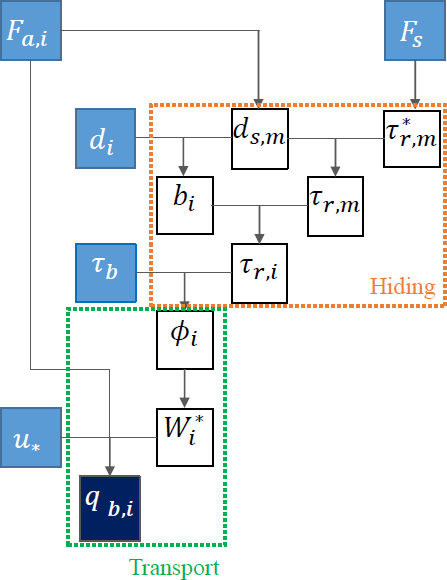
\includegraphics[scale=0.5]{./graphics/Wilcock_application}%
\caption{Scheme of application of the graded sediment transport model of WC-2003. Parameters in blue boxes are input parameters, those in white boxes are intermediary variables computed to estimate the transport rate of size fraction $i$ in the black box.}%
\label{fig:Wilcock_Application}
\end{figure}

Further details on the WC-2003 formula and applications can be found in~\cite{Cordieretal_2019,CORDIER2020103580}.

\noindent

\subsubsection{Engelund-Hansen}
\begin{itemize}
 \item \telkey{BED-LOAD TRANSPORT FORMULA FOR ALL SANDS = 30}
 \item The dimensionless current-induced sediment transport rate is given by:
  \begin{equation*}
  \Phi_b=0.1 \frac{\theta^{\frac{5}{2}}}{c_f}
  \end{equation*}
 with $c_f$ the adimensional friction coefficient and $\theta$ the Shields number without the correction factor for skin friction ($\theta=\frac{\tau_b}{(\rho_s-\rho)gd}$).
 \item Fortran subroutine {\ttfamily bedload\_engel.f}.
\end{itemize}
An exhaustive revision of some common bedload transport formulas and associated information presented in chronological order of development can be found in Table D-2 of~\cite{GarciaBook2006}.
%...............................................................................
\subsection{Modification of the magnitude and direction of bedload}\label{sec:corrections}
%...............................................................................
Three key aspects must be considered for computing the magnitude and direction of the bed load~\cite{Abad08}:
\begin{itemize}
\item[(a)] The effect of the local bed slope
\item[(b)] Secondary flow effects on the direction of the bed shear stress, also refered as to helical flows in the literature
\item[(c)] The bed shear stress partitioning into components affected by skin friction and drag force from bedforms
\end{itemize}
\noindent
\gaia{} includes methods for evaluating these three aspects.

\begin{figure}[H]%
\begin{center}
  \begin{tabular}{ccc}
    \subfloat[]{
      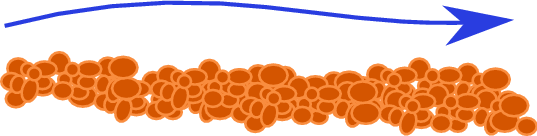
\includegraphics[scale=0.25]{./graphics/transport_1}}&
    \subfloat[]{
      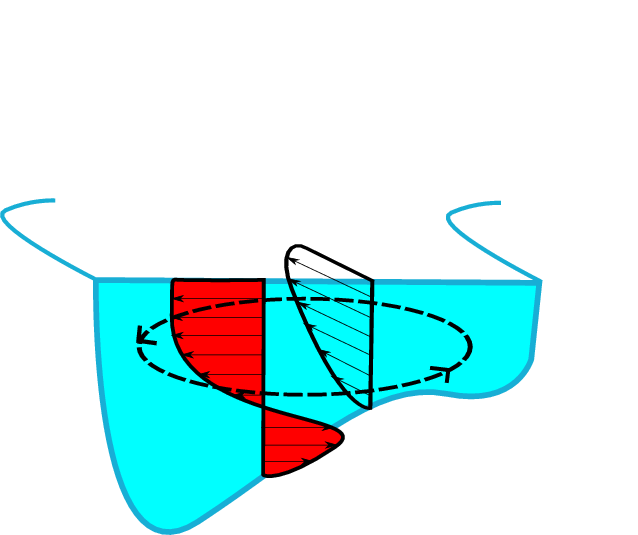
\includegraphics[scale=0.20]{./graphics/curve_4}}&
    \subfloat[]{

\includegraphics[scale=0.75]{./graphics/dunes_drag_grain}}
\end{tabular}
\end{center}
%\caption
%{ADD CAPTION\protect.}
\label{fig:ExampleImage}
\end{figure}

%-------------------------------------------------------------------------------
\subsection{Correction of the direction of the sediment transport}
%-------------------------------------------------------------------------------
The angle $\alpha$ is the angle between the sediment transport direction and the $x-$axis direction will deviate from that of the shear stress by combined action of a transverse slope and secondary currents
In a Cartesian coordinate system, the relation of van Bendegon is:


\begin{minipage}{0.5\textwidth}
\centering
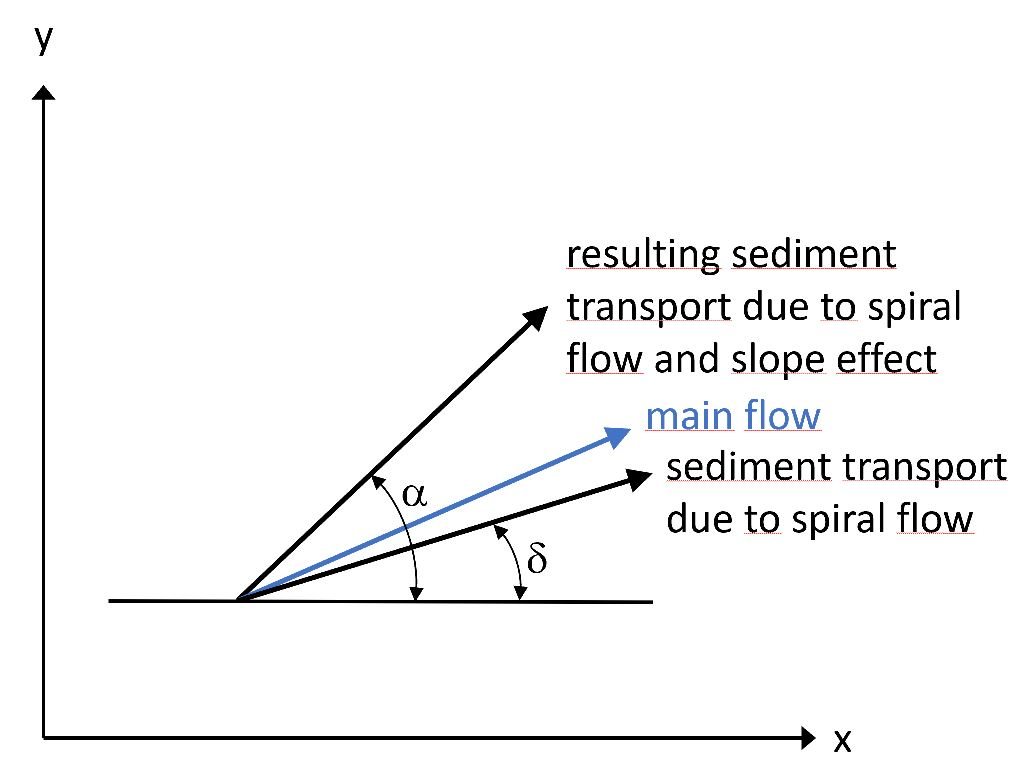
\includegraphics[scale=0.5]{./graphics/sketch_direction_sediment.jpg}%
\end{minipage}
\begin{minipage}{0.5\textwidth}
\begin{equation}
\displaystyle
\tan\alpha = \frac{\sin\delta-\frac{1}{f(\theta)}\frac{\partial z_b}{\partial y}}{\cos\delta-\frac{1}{f(\theta)}\frac{\partial z_b}{\partial x}}.
\end{equation}
\end{minipage}


Above, the terms $\partial z_b/\partial x$ and $\partial z_b/\partial y$ represent respectively the transverse and longitudinal slopes, $z_b$ the bottom position and $\delta$ the angle
between the cartesian coordinate system and the spiral flow. The sediment shape function $f(\theta)$ is a function weighting the influence of the transverse bed slope, expressed as a function of the non-dimensional shear stress or Shields parameter $\theta$. It can be computed according to:

\begin{itemize}
\item Koch and Flokstra~\cite{KochFlokstra80}:
\begin{equation*}
f(\theta) = \frac{3}{2\theta}
\end{equation*}
\item Talmon \textit{et al.}~\cite{Talmon95}:
\begin{equation*}
f(\theta) = \beta_2\sqrt{\theta}
\end{equation*}
where $\beta_2$ is an empirical coefficient. The default value is $\beta_2=0.85$, but an optimal value of $\beta_2=1.6$ was found for the calibration of numerical experiments of dunes and bars in a laboratory channel~\cite{Mendoza15}.
\item Apsley and Stansby~\cite{ApsleyStansby2008}:
\begin{equation*}
f = \frac{\theta_{cr} \cos^2\chi}{\tan\phi}
\end{equation*}
where the slope angle $\cos\chi$ is calculated from the $x$- and $y$-components
of the bed gradient $\cos\chi = 1/\sqrt{1 + (\partial z/\partial x)^2 + (\partial z/\partial y)^2}$ and $\phi$ is the angle of repose.

\end{itemize}

%-------------------------------------------------------------------------------
\subsection{Correction by secondary flow effects on the direction of the bed shear stress}
%-------------------------------------------------------------------------------
In curved channels, the direction of the sediment transport will no longer coincides with the direction of the bed shear stress,
due to the effect of the secondary flows:
\begin{equation}\label{eq:delta}
\delta = \tan^{-1}\left(\frac{v}{u}\right) - \textcolor{red}{\tan^{-1}\left(\frac{A}{r_s}h\right)} = \delta^* - \textcolor{red}{\Delta\delta},
\end{equation}
with $h$ the water depth, $(u,v)$ the components of the depth-averaged velocity field, $r_s$ the local radius of curvature and $A$ the spiral flow coefficient. Above, the term highlighted in red accounts for the effect of the spiral motion on the sediment flux. The angles $\delta^*$ and $\Delta\delta$ indicate respectively the direction of the bed shear stress (which coincides with the direction of the depth-averaged velocity) and the direction due to the effect of secondary currents.

In \gaia{} $A=7^*$ (Engelund's value). Nevertheless, an optimal value of $A=12$ was found for the calibration of numerical experiments of dunes and bars in a laboratory channel~\cite{Mendoza15}.

%-------------------------------------------------------------------------------
\subsection{Correction of the magnitude of the sediment transport}
%-------------------------------------------------------------------------------
The correction of the magnitude of the sediment transport can be computed according to:
\begin{itemize}
\item  Koch and Flokstra~\cite{KochFlokstra80} which is based on the modification of the bed load transport rate by a factor that acts as a diffusion term in the bed evolution equation
\begin{equation}
\begin{array}{ll} \displaystyle
Q_b^* &= Q_{b}\left(1+\beta\frac{\partial z_b}{\partial s}\right) \\
    &= Q_{b}\left[1 + \beta \left(\frac{\partial z_b}{\partial x} \cos\alpha + \frac{\partial z_b}{\partial y} \sin\alpha\right)\right],
\end{array}
\end{equation}
where $s$ is the flow direction and $\beta$ is an empirical factor accounting for the streamwise bed slope effect ($=1.3$ by default).
\medskip

\item Soulsby~\cite{Soulsby97} which s based on the modification of the critical Shields parameter and is therefore only valid for threshold bedload formulas:
\begin{equation*}
\frac{\theta_{\beta cr}}{\theta_{cr}} = \frac{\cos\psi \sin\chi +
\sqrt{\cos^2\chi \tan^2\phi - \sin^2\psi \sin^2\chi}}{\tan
\phi}
\end{equation*}
where $\theta_{\beta cr}$ is the corrected  Shields number for a sloping bed, $\theta_{cr}$ is the critical Shields number for a flat, horizontal bed, $\phi$ is the angle of repose of the sediment, $\chi$ is the bed slope angle with the horizontal, and $\psi$ is the angle between the flow and the bed slope directions.
\medskip

\item  Apsely and Stansby~\cite{ApsleyStansby2008} which is  based on the modification of the critical Shields parameter $\theta_{\beta cr}$ and on the calculation of a effective dimensionless shear stress $\theta_{beta}$.
The modification of the critical shear stress can only be done for threshold bedload formulas. The modification of the Shields parameter $\theta_{\beta}$ could be done for all bedload formulas which are using the shear stress and accordingly the Shields parameter. But it is not recommended.
\begin{equation*}
\frac{\theta_{\beta cr}}{\theta_{cr}} = \cos\chi = 1 / \sqrt{1 + (\partial z /\partial x)^2 + (\partial z/ \partial y)^2 }
\end{equation*}

\begin{equation*}
\theta_{\beta} = \sqrt{\left( \theta \cos\gamma - \frac{\theta_{cr}}{\tan\phi} \frac{\partial z}{\partial x} \cos^2 \chi \right)^2 +
\left(\theta \sin\gamma - \frac{\theta_{cr} }{\tan\phi} \frac{\partial z}{\partial y} \cos^2 \chi \right)^2 }
\end{equation*}
where $\gamma$ is the direction of the bed shear stress.
\end{itemize}



%-------------------------------------------------------------------------------
\subsubsection{Sediment sliding}
%-------------------------------------------------------------------------------
If the bottom slope is higher than a critical slope (typically the angle of repose) sediments can be moved due to geomechanical processes. In \gaia{} two formulas are implemented to calculate sediment displacement in down-slope direction only driven by the bottom slope.
\begin{itemize}

\item The first method is a simple and mass conservative smoothing of the bottom slopes. The changed masses are balanced separately in the mass-balance (MASS EVOLUTION DUE TO SLIDING FORMULA 1).

\item Apsely and Stansby~\cite{ApsleyStansby2008} provide a formulation of avalanching if the bed slope is higher than the angle of repose. In this case the bedload flux  is increased by an additional contribution $q_{aval}$ in the direction of the highest bottom slope. This formula changes the intensity and the direction of the bed load.

\begin{equation*}
q_{aval} = (1-p)\frac{\frac{1}{2} L^2 (\tan\chi - \tan\phi)}{\cos\chi \Delta t}\qquad  \textrm{if} \enspace \tan\chi> \tan\phi
\end{equation*}
\end{itemize}
%-------------------------------------------------------------------------------
\subsection{Keywords for the modification of the intensity and direction of bed load}
%-------------------------------------------------------------------------------
The keyword \telkey{SLOPE EFFECT} (logical type variable, set to {\ttfamily = YES} by default) activates the bed slope effects. If \telkey{SLOPE EFFECT = NO}, the keywords \telkey{FORMULA FOR DEVIATION} and \telkey{FORMULA FOR SLOPE EFFECT} are not taken into account.

%-------------------------------------------------------------------------------
\subsubsection{Correction of the direction of bedload transport}
%-------------------------------------------------------------------------------
The correction of the direction of bedload transport can be done by
\begin{itemize}
\item the Koch and Flokstra formulation \telkey{FORMULA FOR DEVIATION = 1} (integer type variable, set to {\ttfamily = 1} by default),
\item the Talmon et al. formulation \telkey{FORMULA FOR DEVIATION = 2}. This keyword has the associated keyword \telkey{PARAMETER FOR DEVIATION} (real type variable named \telkey{BETA2}, set to {\ttfamily = 0.85} by default).
\item the Apsley and Stansby formulation  \telkey{FORMULA FOR DEVIATION = 3}. This keyword has the associated keyword \telkey{FRICTION ANGLE OF THE SEDIMENT} (real type variable, set to {\ttfamily = 40} by default) and the critical Shields parameter which is calculated by default or can be set with the keyword \telkey{CLASSES SHIELDS PARAMETERS}.
\end{itemize}

%-------------------------------------------------------------------------------
\subsubsection{Correction of the intensity of bedload transport rate}
%-------------------------------------------------------------------------------
The correction of the intensity of bedload transport rate can be done by :
\begin{itemize}
\item the Koch and Flokstra formulation \telkey{FORMULA FOR SLOPE EFFECT} (integer type variable, set to {\ttfamily = 1} by default). This keyword has the associated keyword \telkey{BETA} (real type variable, set to {\ttfamily = 1.30} by default)
\item the Soulsby formulation \telkey{FORMULA FOR SLOPE EFFECT = 2}. This keyword has the associated keyword \telkey{FRICTION ANGLE OF THE SEDIMENT} (real type variable, set to {\ttfamily = 40.} by default) and the critical Shields parameter which is calculated by default or can be set with the keyword \telkey{CLASSES SHIELDS PARAMETERS}.
\item the Apsley and Stansby formulation \telkey{FORMULA FOR SLOPE EFFECT = 3}. This keyword has the associated keyword \telkey{FRICTION ANGLE OF THE SEDIMENT} (real type variable, set to {\ttfamily = 40} by default) and the critical Shields parameter which is calculated by default or can be set with the keyword \telkey{CLASSES SHIELDS PARAMETERS}.
\end{itemize}

%-------------------------------------------------------------------------------
\subsubsection{Correction due to secondary currents}
%-------------------------------------------------------------------------------
The keyword \telkey{SECONDARY CURRENTS} (logical type variable, set to {\ttfamily = NO} by default) accounts for the secondary flow correction. This keyword has the associated keyword \telkey{ SECONDARY CURRENTS ALPHA COEFFICIENT} (real type variable, set to {\ttfamily = 1.} by default) that allows the modification of the coefficient $A$ in Equation~\ref{eq:delta}. This value can be chosen as: $\rightarrow 0.75~~\text{(rough bottom)} \leq \alpha_{SC} \leq 1.0~~\text{(smooth bottom)}$. For example, if $\alpha_{SC} = 1$ then $A = 7$.

%-------------------------------------------------------------------------------
\subsubsection{Correction due to sediment sliding}
%-------------------------------------------------------------------------------
Sediment sliding will be taken into account if the keyword \telkey{SEDIMENT SLIDE}
(integer type variable, set to {\ttfamily = 0} by default) is higher zero:
\begin{itemize}
\item  \telkey{SEDIMENT SLIDE = 1} smoothes the bottom slopes up to the angle of repose.
\item  \telkey{SEDIMENT SLIDE = 2} calculates the sediment sliding with the avalanching formula from Apsley and Stansby.
\end{itemize}
This keyword has the associated keyword \telkey{FRICTION ANGLE OF THE SEDIMENT} (real type variable, set to {\ttfamily = 40} by default)

%-------------------------------------------------------------------------------
\subsection{Influence of the roughness on sediment transport processes}\label{sec:roug}
%-------------------------------------------------------------------------------
%-------------------------------------------------------------------------------
\subsubsection{Skin friction correction}\label{sec:skin}
%-------------------------------------------------------------------------------
The total bed shear stress is due to skin friction and bed form drag but \textbf{only the component due to skin friction acts on bedload}. The shear stress due to skin friction is expressed as:
\begin{equation}\label{eq:taup}
\tau'=\mu\tau_b,
\end{equation}
where $\tau_b = 0.5 \rho C_f (U^2 + V^2)$ is the total bed shear stress and $\mu$ is the friction factor:
\begin{equation}\label{eq:mu}
\mu=\frac{C_f'}{C_f}
\end{equation}
where $C_f$ is the friction coefficient due to form drag plus skin friction (specified in the hydrodynamics module), and $C_f'$ is the friction coefficient due only to skin friction, which is computed as:
\begin{equation}\label{eq:cfp}
C_f'=2\left(\frac{\kappa}{\log(12h/k_s')}\right)^2,
\end{equation}
where $\kappa$ is the von K\'arm\'an coefficient ($=0.40$), the roughness height $k_s'=\alpha_{k_s}d_{50}$, the coefficient $\alpha_{k_s}$ is a calibration parameter.

%-------------------------------------------------------------------------------
\subsubsection{Keywords for skin friction correction}
%-------------------------------------------------------------------------------
The keyword \telkey{SKIN FRICTION CORRECTION} (integer type variable, {\ttfamily = 1} by default) activates the correction of the bed shear stress due to skin friction:
\begin{itemize}
\item If \telkey{SKIN FRICTION CORRECTION = 0}, then $\mu=1$ and the total bed shear stress issued from the hydrodynamics computation is used
\item If \telkey{SKIN FRICTION CORRECTION = 1}, $\mu$ is computed according to Equation~\ref{eq:mu}. In this case, the friction coefficient $C_f$ is provided by the hydrodynamics steering file and $C_f'$ is computed by Equation~\ref{eq:cfp}. To compute $k_s'=\alpha_{k_s} d_{50}$, the coefficient $\alpha_{k_s}$ can be modified with the keyword \telkey{RATIO BETWEEN SKIN FRICTION AND MEAN DIAMETER} (real type variable, {\ttfamily = 3.} by default). In the numerical experiments of Mendoza \textit{et al.}~\cite{Mendoza15}, $\alpha_{k_s}=37$ for dunes and $\alpha_{k_s}=3.6$ for bars.

 \begin{WarningBlock}{Note:}
  By default, the keyword \telkey{SKIN FRICTION CORRECTION = 1}. In the presence of very shallow waters, this correction can present stability issues. For this case, we suggest the user to set the keyword \telkey{SKIN FRICTION CORRECTION = 0}.
  \end{WarningBlock}

\item If \telkey{SKIN FRICTION CORRECTION = 2}, the presence of ripples is taken into account to compute $\mu$ (see subroutine \texttt{tob\_gaia.f}). For this option, a bedform predictor is used to calculate the bedform roughness $k_r$ in order to account for the effect of ripples. Both $k_r$
and $k_s'$ should influence the transport rates. It is assumed that:
\begin{equation}\label{eq:mu2}
\mu =\frac{C_f'^{0.75} C_r^{0.25}}{C_f},
\end{equation}
where the quadratic friction $C_r$ due to bedforms is calculated as a
function of $k_r$ (see \S~\ref{sec:bedroughpredictor}).
\end{itemize}

%-------------------------------------------------------------------------------
\subsection{Bed roughness predictor}\label{sec:bedroughpredictor}
%-------------------------------------------------------------------------------
A natural sediment bed is generally covered with bedforms, with length $\lambda_d$ (m)
and height $\eta_d$ (m). The presence of bed forms greatly modifies the boundary
layer flow structure, with the formation of recirculation cells and
depressions in the lee of bedforms.\\

Depending on the flow and sediment transport rates, the size of bed
forms ranges from a few centimeters for ripples to a few tens of meter for
mega-ripples. The dimension of dunes scales with the water depth $h$, such that $\eta_d
\approx 0.4 h$ and  $\lambda_d\approx [6-10] h$.\\

In most cases, large scale models do not resolve the small to medium
scale bedforms (such as ripples or mega-ripples) which need therefore to be parameterized by increasing the friction coefficient. To determine bed roughness, there are two options available in \gaia{}:
\begin{itemize}
\item By imposing the friction coefficient based on friction laws: in this case the values of the friction coefficients are provided by \telemac{2D} or \telemac{3D}.
\item By predicting the value of the bed roughness as a function of flow and sediment parameters using a bed roughness predictor. This option is discussed below.
\end{itemize}
Different options are programmed in \gaia to predict the total bed
roughness through the associated keywords \telkey{COMPUTE BED ROUGHNESS AT SEDIMENT SCALE} (logical type variable, set to {\ttfamily = NO} by default) and \telkey{BED ROUGHNESS PREDICTOR OPTION}. The calculated Nikuradse value for the total bed roughness is given to the hydrodynamics. Therefore, the Nikuradse friction law must be selected in the hydrodynamics. The roughness coefficient of the hydrodynamic is only changed for nodes with movable bed.
% no stand alone option for GAIA anymore!
%It is recalled that the bed friction option of \gaia is not
%used in the case of internal coupling with \telemac{2D} or \telemac{3D}.
\begin{itemize}
\item For {\ttfamily BED ROUGHNESS PREDICTOR OPTION = 1}: the bed is assumed to be flat $k_s = k_s'= \alpha_{k_s} d_{50}$, with $\alpha_{k_s}$ a constant (assumed to be equal to $3.$), modified by the keyword \telkey{RATIO BETWEEN SKIN FRICTION AND MEAN DIAMETER}.
\item {\ttfamily BED ROUGHNESS PREDICTOR OPTION = 2}: the bed is assumed to be covered by ripples.
  \begin{itemize}
    \item For currents only, the ripple bed roughness is function of the mobility number, see~\cite{vanRijn07}:
\begin{equation*}
k_r =\left\{\begin{array}{ll}
d_{50}(85-65\tanh(0.015(\Psi-150))) & \text{for\,} \Psi<250\\
20 d_{50} & \text{otherwise}
\end{array}
\right.
\end{equation*}
with $\Psi =U^2/(s-1)gd_{50}$.

    \item For waves and combined waves and currents, bedform dimensions are calculated
as a function of wave parameters following the method of Wiberg and Harris~\cite{WibergHarris}.
The wave-induced bedform bed roughness $k_r$ is calculated as a function of the wave-induced bedform
height $\eta_r$:
\begin{equation}
k_r = \max(k_s', \eta_r).
\end{equation}
Then $k_s=k_s'+k_r$.
  \end{itemize}

\item {\ttfamily BED ROUGHNESS PREDICTOR OPTION = 3}: for currents only, the van Rijn's total bed roughness predictor~\cite{vanRijn07, Huybrechts} has been implemented.
The total bed roughness can be decomposed into a grain
roughness $k_s'$, a small-scale ripple roughness $k_r$, a mega-ripple
component $k_{mr}$, and a dune roughness $k_d$:
\begin{equation}\label{eq:totalbedroughness}
k_s = k_s' + \sqrt{k_r^2 + k_{mr}^2 + k_d^2}.
\end{equation}
Both small scale ripples and grain roughness have an influence on the
sediment transport laws, while the mega-ripples and dune roughness only
contribute to the hydrodynamic model (total friction). In Equation~\ref{eq:totalbedroughness}, the general expression for megaripples roughness $k_{mr}$ is given by:
\begin{equation}
k_{mr} = 0.00002\,f_{ts}\,h\,(1-\exp^{-0.05\Psi})\,(550-\Psi),
\end{equation}
with
\begin{equation*}
f_{ts} =\left\{\begin{array}{ll}
d_{50}/(1.5d_{sand}) & \text{for\,} d_{50}\leq 1.5d_{sand}\\
1.0 & \text{otherwise}
\end{array}
\right.
\end{equation*}
and the general expression for dune roughness $k_d=0.00008\,f_{ts}\,h\,(1-\exp^{-0.02\Psi})\,(600-\Psi)$.

\end{itemize}

%-------------------------------------------------------------------------------
\subsection{Boundary conditions for bedload}
%-------------------------------------------------------------------------------
The specification of boundary conditions is done in a boundary condition file, usually named with extension \texttt{*.cli}. The reader is referred to \S\ref{sec:flags} for the definition of the different flags used in the boundary condition file.

\subsubsection{Wall boundary conditions}
At banks and islands, the bedload transport rate is set to zero. For this case, the flag \texttt{LIEBOR} is set \texttt{= 2} as shown in the example below:

\begin{lstlisting}[frame=trBL]
2 2 2 0.0 0.0 0.0 0.0 (*@\color{PantoneRed}2@*) 0.0 0.0 0.0 565 1
\end{lstlisting}

\subsection{Inflow boundary conditions}
In a depth-averaged 2D sediment transport model, the sediment discharge must be given at each point of the inflow boundary. The different cases can be present:
\subsubsection{Equilibrium sediment discharge}
For this case, the flag \texttt{LIEBOR} is set \texttt{= 5} and the flag \texttt{EBOR} is set \texttt{= 0.0} (no bottom change at the inflow boundary) as shown in the example below:

\begin{lstlisting}[frame=trBL]
4 5 5 0.0 0.0 0.0 0.0 (*@\color{PantoneRed}5@*) (*@\color{PantoneRed}0.0@*) 0.0 0.0 565 1
\end{lstlisting}

\subsubsection{Constant sediment discharge in time}
For this case, boundary condition files are needed for both \telemac{2D} and \gaia{}. In the \gaia{}'s boundary condition file, the flag \texttt{LIQBOR = 5} and \texttt{LIEBOR = 4}. The imposed solid discharge can be specified as follows:
\begin{itemize}
\item A value of the unit solid discharge [kg/(m~s)] in the column \texttt{Q2BOR} of the \gaia{}'s boundary condition file, as shown in the example below for an imposed unit discharge \texttt{Q2BOR=}$1.0$~kg/(m~s):
\begin{lstlisting}[frame=trBL]
4 (*@\color{PantoneRed}5@*) 5 (*@\color{PantoneRed}1.0@*) 0.0 0.0 0.0 (*@\color{PantoneRed}4@*) 0.0 0.0 0.0 565 1
\end{lstlisting}

Particular cases of \texttt{Q2BOR} can be programmed in the subroutine \texttt{conlit.f}.

\item A value of the total solid discharge (without pores) [kg/s] given through the keyword \telkey{PRESCRIBED SOLID DISCHARGES} (sequence of real values separated by semi-colons, one value per liquid boundary, no default value) in the steering file, as shown in the example below for an imposed total discharge equal to $10.0$~kg/s:
\begin{lstlisting}[frame=trBL]
4 (*@\color{PantoneRed}5@*) 5 1.0 0.0 0.0 0.0 (*@\color{PantoneRed}4@*) 0.0 0.0 0.0 565 1
\end{lstlisting}
\begin{lstlisting}[frame=trBL]
PRESCRIBED SOLID DISCHARGES : 10.0
\end{lstlisting}
When a value of solid discharge is given in the parameter file, \texttt{Q2BOR} is considered as only a profile (so it must be greater than 0.). For a constat profile, values equal to 1.0 (as here above) must be filled in.

\end{itemize}

\subsubsection{Time-series of sediment discharge}
Time-series values of sediment discharge are specified in a file through the keyword \telkey{LIQUID BOUNDARIES FILE} (character type), declared in the hydrodynamic steering file. The \gaia{}'s boundary condition file must contain the flags as shown below:
\begin{lstlisting}[frame=trBL]
4 (*@\color{PantoneRed}5@*) 5 1.0 0.0 0.0 0.0 (*@\color{PantoneRed}4@*) 0.0 0.0 0.0 565 1
\end{lstlisting}

The keyword \telkey{PRESCRIBED SOLID DISCHARGES} must be also included in the steering file, with an arbitrary value.

\subsubsection{Repartition of imposed sediment discharge in case of graded
distributions}
In case of several classes of non-cohesive sediments, the sediment discharge can
 be subdivided to the various classes through the keyword
\telkey{CLASSES IMPOSED SOLID DISCHARGES DISTRIBUTION} (sequence of real values
separated by
semi-colons, one value per class whose sum is equal to 1.).

In cases where this keyword is not used, the sediment discharge will be
subdiveded among the various classes according to the sand ratio computed
by \gaia.

\subsection{Outflow boundary conditions}
At the outflow boundary, bedload does not require any particular boundary condition.
For this case, the flag \texttt{LIEBOR} is set \texttt{= 4} as shown in the example below:

\begin{lstlisting}[frame=trBL]
5 4 4 0.0 0.0 0.0 0.0 (*@\color{PantoneRed}4@*) 0.0 0.0 0.0 565 1
\end{lstlisting}

%-------------------------------------------------------------------------------
\subsection{Useful graphical printouts for bedload}
%-------------------------------------------------------------------------------
Through the keyword \telkey{ VARIABLES FOR GRAPHIC PRINTOUTS}, some useful printouts for bedload sediment transport are listed below:
\begin{lstlisting}[frame=trBL]
TOB="Bed shear stress(N/m2)";
MU ="Skin friction coefficient";
M="bed-load discharge (kg/(m*s)";
N="bed-load discharge along x axis (kg/(m*s))";
P="bed-load discharge along y axis (kg/(m*s))";
E="bottom evolution (m)";
QSBL="bed load transport rate (kg/(m*s))";
\end{lstlisting}

\begin{WarningBlock}{Note:}
The sediment discharge is the mass of sedimentary material, both particulate and dissolved, that passes across a given flow-transverse cross section of a given flow in unit time. The flag {\ttfamily M} accounts for the total solid discharge (bedload plus suspended load), while {\ttfamily QSBL} accounts for the bed load solid discharge. If suspended load is not taken into account in the simulation, the output values of {\ttfamily M} and {\ttfamily QSBL} are equivalent.
\end{WarningBlock}
%-------------------------------------------------------------------------------
\subsection{Useful graphical printouts for continuing a computation}
%-------------------------------------------------------------------------------
As for the module \telemac{2D}, in \gaia{} it is possible to continue a computation, taking a time step of a previous computation, on the same mesh as initial state.
As well as for the hydrodynamic part, it is necessary to declare two keywords in the steering file:
\begin{enumerate}
\item \telkey{COMPUTATION CONTINUED}, which must be set equal to YES
\item \telkey{PREVIOUS SEDIMENTOLOGICAL COMPUTATION FILE}, to give the name of the file that will supply the initial state.
\end{enumerate}
When continuing a computation it is important that the previous sedimentological computation file contains the appropriate variables in order to properly continue the computation. Below some advices are introduced:

\begin{WarningBlock}{Note:}
\begin{itemize}
\item the bottom (B) and the layer thickness (*ES) are mandatory
\item the non erodable bottom (R) is optional since when missing, it is computed using the layer thickness
\item the masses are mandatory to continue the computation, so:
\begin{itemize}
 \item if the variables *S* (or *M*) are saved in the previous file, they will be directly taken for continuing computation
 \item if the previous file does not contain masses, they will be reconstructed using the ratios (*A*,*R*) and the porosity, as well as the thickness.
\end{itemize}
\end{itemize}
\end{WarningBlock}

These suggestions are necessary only when the
\telkey{PREVIOUS SEDIMENTOLOGICAL COMPUTATION FILE} is manually generated by
users (as result file of a previous computation).
Indeed, since release v8.5, the new feature \telkey{RESTART MODE} for \gaia{}
has been introduced and described in \ref{sec-restart} to facilitate computation
continuing when using \gaia{}.

%
%the following is to do
%-------------------------------------------------------------------------------
%\subsection{Non-uniform sediment distribution}
%-------------------------------------------------------------------------------

\pagebreak
%-------------------------------------------------------------------------------
\section[Bottom stratigraphy]{Bottom stratigraphy}
%-------------------------------------------------------------------------------
For sand graded distributions, an algorithm based on the classical active layer formulation of Hirano is used~\cite{doi:10.1029/2006WR005474}. The active layer supplies material that can be eroded or deposited as bedload or suspended load. Its thickness can be specified by the user or set by default to the value $3\times d_{50}$, with $d_{50}$ the median diameter of sediment material contained in the active layer.

The bed model can be discretized by a constant number of layers along the vertical direction. Since layers are allowed to be emptied, the utilized number of layers at each mesh node can vary during a numerical simulation. When more than one sediment class is specified in the steering file, the following cases arise: ($i$) for a given initial bed stratification (i.e. through a given number of layers $N_{lay}$), an active layer is added inside this stratification at the beginning of the simulation. In this case the total number of layers is $=N_{lay}+1$; ($ii$) if the initial bed stratification is not provided, the sediment bed is thus subdivided in two layers: the active layer and a substrate layer located directly below. In this case, the total number of layers is $=2$.

To maintain a constant active layer thickness throughout the numerical simulation, at each time step the following procedures are performed:
\begin{itemize}
    \item In the case of erosion, the sediment mass is taken from the active layer, therefore the sediment flux is transferred from the substratum (first non-empty layer below the active layer) to the active layer. Note that the rigid bed algorithm is applied to the active layer, i.e.~only the sediment mass in the active layer is available at the given time step. This is important as bedload transport rate and/or the rate of entrainment for suspension are computed using the sediment composition available in the active layer.
    \item If the erosion during the time step exceeds the sediment mass available in the top layer, this layer is fully eroded and a new erosion rate is computed using the composition of the layer underneath, that is now the surface layer.
    \item In the case of deposition, the increased thickness generates a sediment flux from the active layer to the first substratum layer. %CHECK!!!
\end{itemize}

The bed model algorithm introduced before has been modified to account for the presence of mud or sand-mud mixtures.
Mixed sediment consists of a mixture of $N_{nco} \geq 1$ classes of non-cohesive sediment (sand and/or gravel) with $N_{co} \geq 1$ classes of fine, cohesive sediment. Non-cohesive sediments are assumed to be transported by bedload and/or suspension, while cohesive sediment is transported only by suspension.

In the algorithm for mixed sediments, the layer thickness results from the mass ratio of cohesive and non-cohesive sediment contained in each layer. If the cohesive sediment volume is $\leq 40\%$ of the non-cohesive sediment volume, the layer thickness only depends on the mass of non-cohesive sediment volume. Conversely, if the cohesive sediment volume is $\geq 40\%$ of the non-cohesive sediment volume, the layer thickness is computed from the non-cohesive sediment volume plus the cohesive sediment volume minus the interstitial volume between non-cohesive sediment classes.

The presence of high concentrations of cohesive sediment in the bed are known to prevent bedload transport from occurring~\cite{vanLedden}. Therefore, in \textsc{Gaia}, bedload transport is only computed if the mass fraction of cohesive sediment in the active layer is $\leq 30\%$. In this case, the non-cohesive sediment can still be transported in suspension. In addition, erosion of non-cohesive sediment by bedload transport causes cohesive sediment present in the mixture to be entrained into suspension.


%-------------------------------------------------------------------------------
% This section gives a description of the former hippodrome test case
%%\subsection{Preliminaries}
%%%-------------------------------------------------------------------------------
%%The general bed model implemented in \gaia{} is used to compute both both horizontal and vertical spatial and temporal variability of bed mixture composition (in the case of more than one sediment class, representing graded and/or mixed sediment) and/or sediment properties (in the case of consolidation of cohesive sediment).
%%
%%The two simplest cases of the bed model, namely the variability of bed mixture composition, based on the active layer model for non-cohesive sediment, and the consolidation model for one sediment class, are presented in sections~\ref{bedmodel:active} and \ref{}, respectively. A more general case is introduced later in section~\ref{}, including:
%%\begin{itemize}
%%\item mixed sediment (cohesive and non-cohesive sediment)
%%\item consolidation of more than one cohesive sediment
%%\item mixed sediment with consolidation
%%\end{itemize}
%%
%%For all cases, the bed model consists of a discretization of the sediment bed over the vertical direction through a user-defined fixed number of bed layers. Although the number of bed layers is kept constant for the whole computation domain, they can empty during the simulation time, leading to a ``merging'' of layers sharing the same interface.
%%
%%The main variable used in the code to represent the amount of sediment in each layer is the sediment mass for each sediment class (variables \texttt{MASS\_MUD(IMUD,ILAYER,IPOIN)} and \texttt{MASS\_SAND(ISAND,ILAYER,IPOIN)} for cohesive and non-cohesive sediment, respectively). The following sediment transport processes can modify the sediment mass contained in each layer:
%%\begin{itemize}
%%\item Bedload transport (for non-cohesive sediment only),
%%\item Suspended sediment transport,
%%\item Sediment ``avalanching'', due for example to the collapse of bed slope over a critical slope or angle of repose,
%%\item Consolidation (for cohesive sediment only).
%%\end{itemize}
%%
%%For each time step, the bed model algorithm updates:
%%\begin{itemize}
%%\item the bed layer thicknesses and therefore the bed elevation, computed as the sum of the rigid bed elevation plus the layer thicknesses
%%\item the variables representing the sediment bed composition, namely:
%%  \begin{itemize}
%%  \item the mass fraction of each class of cohesive sediment over the total cohesive sediment mass (variable \texttt{RATIO\_MUD(IMUD,ILAYER,IPOIN)})
%%  \item the mass fraction of each class of non-cohesive sediment over the total non-cohesive sediment mass (variable \texttt{RATIO\_SAND(ISAND,ILAYER,IPOIN)}),
%%  \item the mass fraction of cohesive sediment over the total sediment mass (cohesive and non-cohesive)
%%  \end{itemize}
%%\end{itemize}
%%
%%\begin{WarningBlock}{Note:}
%%There is no choice of bed model to be made by the user. It is automatically selected by the code depending on the processes, and type and number of sediment classes set by the user in the \gaia{}'s steering file.
%%\end{WarningBlock}

%-------------------------------------------------------------------------------
\subsection{Active layer model}\label{bedmodel:active}
%-------------------------------------------------------------------------------
The active layer is the surface layer, which supplies material that can be transported as bedload or suspended load and receives the deposited sediment material. Therefore the composition of the active layer is used to compute the rate of bedload transport and the rate of erosion in suspension for each sediment class, where decomposition of bedload transport and suspension transport in size-classes is presented. This composition is variable in space and time as it depends on the composition of the sediment deposited and/or eroded from this layer, as well as the exchange of mass with the substratum.

The active layer thickness depends on the flow and sediment characteristics. In \gaia{}, the active layer thickness is constant, with a target value set by the user. The active layer thickness can be internally modified during the simulation.

At the beginning of the computation, if there is more than one sediment class set in the steering file, the active layer is created automatically at the surface of the sediment bed.

\begin{itemize}
\item In the case where the user does not set any initial bed stratification (i.e. the initial bed material composition is set constant over the vertical direction), the sediment bed is subdivided in two layers: an ``active'' or ``mixing'' layer in contact with the water column, and a substrate layer located immediately below.
\item In the case where the user does set an initial bed stratification (i.e. layers of different bed compositions, see chapter \ref{chap:how-to}), then:
  \begin{itemize}
  \item An active layer will be added inside this stratification at the beginning of the computation. Therefore, the actual number of layers will be equal to the number of layers for the initial stratification plus one.
  \item If the first (surface) layer of the initial stratification is larger than the target active layer thickness, this surface layer is split in two sub-layers: the active layer plus a layer immediately below with a thickness equal to the first stratification layer thickness minus the active layer thickness. For this case, the initial composition of the active layer is assumed to be the same as the composition of the first layer.
  \item If the first (surface) layer of the initial stratification is smaller than the target active layer thickness, the active layer is ``merged'' by the first layer, and also take from the stratification layer(s) underneath the remaining amount of sediment necessary to reach its target thickness. The initial composition of the active layer will thus be a mix of the sediment from the first and (partially) the second stratification layers.
  \end{itemize}
\end{itemize}

If during a simulation, the thickness of sediment available in the bed is smaller than the target active layer thickness, the actual active layer thickness for this node will be equal to the sediment thickness. All sediment in the bed will thus be mixed in the active layer. The target active layer thickness is thus only respected if there is enough available sediment. This enables smooth implementation of the rigid bed algorithm also for the case of the active layer model. This point is also important as it enables the user to ``force'' a full mixing of sediment composition over the whole sediment thickness by imposing a very large target active layer thickness (see chapter \ref{chap:how-to}). At each time-step, the substratum exchanges material with the active layer in order to keep the active layer at a target thickness:

\begin{itemize}
\item In the case of erosion, mass is taken from the active layer to be sent in suspension, or to the active layer of neighbouring nodes (through bedload). Therefore, to keep active layer thickness at a target value, the sediment mass has to be transferred from the substratum (first non-empty layer below the active layer plus layers underneath if necessary) and incorporated into the active layer. The mass transferred has the composition of the substratum: this correction flux does not change the composition of the substratum but might change the composition of the active layer. Note that the rigid bed algorithm is applied to the active layer, i.e. only the mass of sediment in the active layer is available for erosion during a given time-step. Therefore the amount of erosion during a time-step should not exceed the amount of mass in the active-layer (this is important for physical coherence as the bedload transport rate as well as the rate of erosion in suspension are computed using the composition of the active layer).

\item In the case of deposition, mass is added to the active layer. Therefore a flux of sediment mass has to be taken from the active layer and added to the substratum (first non-empty layer below the active layer). The mass transferred has the composition of the active layer: this correction flux does not change the composition of the active layer but might change the composition of the substratum. No bookkeeping of the composition of deposits, that is the creation of new layers of substratum to discretize the deposits, has been implemented for the current version of \gaia{}.
\end{itemize}

%-------------------------------------------------------------------------------
The active layer model is automatically selected when there are at least two size-classes of sediment (set by the dimension of keyword \texttt{CLASSES TYPE OF SEDIMENT}).
By default, the composition of the sediment mixture is constant over the computational domain and set by keyword \texttt{CLASSES INITIAL FRACTION}.
The target active layer thickness is set by the keyword \texttt{ACTIVE LAYER THICKNESS}.

The user might wish not to use the active layer model, and thus to mix the sediment composition on the sediment bed, resulting in one sediment layer. For this case, the user can set a target active layer thickness value larger than the maximum sediment layer thickness. Note that this is the default case, since the default value for keyword \texttt{ACTIVE LAYER THICKNESS} is equal to 10,000 m, while the default value for sediment thickness is equal to 100 m (as hardcoded in \texttt{lecdon\_gaia}). This value can be modified with the keyword \texttt{LAYERS INITIAL THICKNESS}).

To set a variable bed composition along the vertical direction, the keyword \texttt{NUMBER OF LAYERS FOR INITIAL STRATIFICATION} can be used.

Layers thicknesses and compositions must be set using the variables \texttt{ESTRATUM(ISTRAT,IPOIN)} and \texttt{RATIO\_INIT(ICLA,ISTRAT,IPOIN)}. The same user subroutine must be used to set spatially-dependent bed compositions.

%-------------------------------------------------------------------------------
\subsubsection{Mixed sediment}
%-------------------------------------------------------------------------------
Mixed sediment is defined as the mixture of \texttt{Nnco} classes ($Nnco \geq 1$) of non-cohesive sediment (e.g.~sand and/or gravel) and \texttt{Nco} classes ($Nnco \geq 1$) of fine, cohesive sediment (e.g.~mud). The non-cohesive sediment is transported by bedload and/or suspension, and the cohesive sediment is transported only by suspension. The bed model is a generalization of the active-layer bed model implemented for non-cohesive sediment, as follows:

\begin{enumerate}
\item The composition of the surface layer (the active layer) of the bed sediment mixture is considered for computing the critical shear stress for erosion, the bedload transport rate, and the erosion rate in suspension.
\item Each layer's thickness, and thus the resulting bed elevation at the end of each time step, is computed from the mass of non-cohesive sediment and cohesive sediment using the following hypothesis:
\begin{itemize}
\item If the cohesive sediment volume is smaller than 40\% of the non-cohesive sediment volume, the layer thickness is only function of non-cohesive sediment mass.
\item If the cohesive sediment volume is larger than 40\% of the non-cohesive sediment volume, the layer thickness is computed from non-cohesive sediment volume plus cohesive sediment volume minus interstitial volume between non-cohesive sediment grain sizes.
\end{itemize}
\item For several cohesive sediment classes in the mixture, it is assumed that each sediment class has its own settling velocity value.
%  \begin{itemize}
%    \item They have the same critical shear stress and their erosion fluxes are computed in the same way. The actual erosion fluxes takes into account the availability of each class in the surface layer, therefore the erosion fluxes of the classes of cohesive sediment can in fact be different.
%    \item In the case of consolidation, the consolidation fluxes are computed in the same way for all classes. Therefore, consolidation fluxes from one layer to the more consolidated layer underneath can be different between classes only because of the different availability of each class in the layer considered.
%  \end{itemize}
%When there is consolidation, the following two points apply:
%\item Each layer of the bed model accounts both for:
%	Temporal and spatial (horizontally and vertically) variation of the properties of the cohesive sediment (critical shear stress, Partheniades constant and consolidation rate) as in the consolidation bed model.
%	Temporal and spatial (horizontally and vertically) variation of the composition of the sediment mixture (\% of each class of non-cohesive sediment and cohesive sediment in the mixture) as in the active layer bed model.
%\item The properties (critical shear stress, Partheniades constant and consolidation rate) of the cohesive sediment in the surface (active) layer are interpolated. This consists in aggregating the surface layers of the bed model over a predefined active layer thickness. %The composition of the mixture of this active layer is then used to interpolate (to continue) - RWR
%
%  In the case of mixed sediment, non-cohesive sediment presence in the mixture is considered to not alter cohesive sediment consolidation. Non-cohesive sediment is ``trapped'' by cohesive sediment when cohesive sediment consolidates. Thus transfer of cohesive sediment from one layer to the layer underneath is accompanied by a transfer of non-cohesive sediment. The non-cohesive sediment/cohesive sediment ratio of the transferred sediment is the same as the ratio of consolidating layer. If there are more than one classes of non-cohesive sediment, they are transferred according to their percentage of presence in the consolidating layer.
\end{enumerate}

%\subsubsection{Deposition}
%Flux of non-cohesive sediment deposits from the water column can be considered to immediately settle through the fresh cohesive sediment and thus is added to the mass of non-cohesive sediment of the layer of the consolidation bed model. In this case there can be no non-cohesive sediment is the first upper layers of the bed model. Is there possibility to bypass the first layer (yes in the fortran, no keyword).

%\subsubsection{Erosion}
%At each time step, the surface composition of the sediment bed is used to compute the critical shear stress for erosion and the rate of erosion in suspension (for cohesive sediment and all non-cohesive sediment classes). The composition considered is the one of the surface (active) layer.

Following~\cite{LEHIR2011S135}, the critical shear stress for a mass cohesive sediment fraction of the mixture is computed as follows.

If the mass cohesive sediment fraction of the mixture is:
\begin{itemize}
\item $>50\%$, its value is equal to the critical shear stress of the cohesive sediment fraction (that depends on cohesive sediment concentration)
\item $<30\%$, its value is equal to the critical shear stress of the non-cohesive sediment fraction, with a correction that increases the critical shear stress to account for the cohesive sediment fraction
\item in the range $[30-50]\%$, its value is computed by linear interpolation of values computed from the two previous cases.
\end{itemize}

If the erosion rate for a mass cohesive sediment fraction of the mixture is:
\begin{itemize}
\item  $>50\%$, its value is equal to the erosion rate for cohesive sediment fraction
\item $<30\%$, its value is equal to the erosion rate computed for the non-cohesive sediment fraction
\item in the range $[30-50]\%$, its value is computed by linear interpolation of values computed from the two previous cases.
\end{itemize}

%The total erosion rate is then distributed among non-cohesive sediment and cohesive sediment fractions, according to their respective fraction in the mixture.
%Encore d’actualité ? Vérifier ?
%If erosion during the time step exceeds the mass of sediment  present in this top layer (for cohesive sediment and all non-cohesive sediment classes), the layer is fully eroded, and the duration needed for this full erosion is substracted from the time step. A new erosion rate is then computed using the composition of the layer underneath, that is now the new surface layer. This erosion rate is applied to the new surface for what remains of the duration of the time step. Again, if the erosion exceed the mass in this layer, the layer underneath will be considered for erosion, etc.

\subsubsection{Bedload}
Bedload transport is computed only if mass cohesive sediment fraction in the active layer is lower than 30\%. Otherwise, non-cohesive sediment can still be transported in suspension. Erosion of non-cohesive sediment through bedload causes cohesive sediment present in the mixture to be entrained in suspension. As for deposit from suspension, deposit of non-cohesive sediment caused by bedload is added to the third layer of the consolidation bed model (corresponding to a sediment concentration equal to 100 g/l).







\pagebreak
%-------------------------------------------------------------------------------
\section{Consolidation processes}
%-------------------------------------------------------------------------------
For the current version of \textsc{Gaia}, consolidation processes are based on the semi-empirical formulation originally developed by Villaret and Walther~\cite{VillaretWalther2008}, which uses the iso-pycnal and first-order kinetics formulations. Consolidation of mud deposits is modeled using a layer discretization, where the first layer corresponds to the freshest deposit, while the lower layer is the most consolidated layer. Sediment deposition from the water column is added directly to the first layer.
A rate (or \textit{flux}) of consolidation is computed for each layer and for each class of cohesive sediment separately. The values of the computed fluxes depend on the availability of each class in the layer considered.

%The keyword {\ttfamily MUD CONSOLIDATION} (logical type, set to {\ttfamily = NO} by default) activates consolidation processes in \gaia{}. Two different models for consolidation are available with the keyword {\ttfamily CONSOLIDATION MODEL} (logical type, set to {\ttfamily = 1} by default):
Consolidation can be activated using the keyword \telkey{BED MODEL = 2} (integer type variable, set to {\ttfamily = 1} by default).

%\begin{itemize}
%\item Multilayer model ({\ttfamily = 1}): This model was originally developed by Villaret and Walther~\cite{} by mixing two
%approaches of iso-pycnal and first-order kinetics. In this model, the muddy bed is discretised into a fixed number of layers.
%Each layer $j$ is characterised by its mass concentration $C_j$ [kg/m$^3$], its mass per unit surface $M_s(j)$
%[kg/m$^2$], its thickness $ep_j$ [m] and a set of mass transfer coefficient $a_j$ (s$^{-1}$). This empirical model assumes that the vertical flux of
%sediment from layer $j$ to underneath layer $j+1$ is proportional to the mass of sediments $M_s(j)$ contained in the layer $j$.
%
%\item The Gibson/Thiebot's model ({\ttfamily = 2}): This is a 1DV sedimentation-consolidation multi-layer model, based on an original
%technique to solve the Gibson equation, developed by Thiebot et al.~\cite{thiebot08}. The advantage of
%this representation is that the flux of sedimentation and consolidation is calculated based on
%the Gibson theory. In this model, the concentration of different layers are fixed, the associated thicknesses are directly
%linked to the amount of sediment that they contain. The scheme of this model is similar to the multilayer model.
%However, instead of using the transfer coefficients which are
%arbitrary, this model is based on the Gibson's theory for the definition of the settling velocity
%of solid grains and the determination of mass fluxes
%\end{itemize}

\subsection{Associated keywords for consolidation models}
\begin{itemize}
\item Multilayer model (\telkey{BED MODEL = 2})
\begin{itemize}
\item {\ttfamily LAYER MASS TRANSFER} (real list, set to {\ttfamily = 5.D-05;4.5D-05;...} by default) provides the mass transfert coefficients of the multilayer consolidation model (in s$^{-1}$)
\end{itemize}
%\item For the Gibson/Thiebot's model ({\ttfamily = 2}), the following values are used in the closure relationship equation for the permeability:
%\begin{itemize}
%%\item {\ttfamily GEL CONCENTRATION} (real type, set to {\ttfamily = 310.D0} kg/m$^3$ by default) is the transition concentration between the sedimentation and consolidation schemes
%%\item {\ttfamily MAXIMUM CONCENTRATION} (real type, set to {\ttfamily = 364.D0} kg/m$^3$ by default) is the maximum concentration for the Gibson/Thiebot's model
%%\item {\ttfamily PERMEABILITY COEFFICIENT} (real type, set to {\ttfamily = 8.D0} by default) %CHECK IF OK FOR MODEL 2 AND UNITS?
%\end{itemize}
\end{itemize}

Further information about both models can be found in~\cite{Lan12}.

The parameters per layer of the consolidation (cohesive sediment concentration, critical erosion shear stress, and rate of mass transfer to the layer underneath) model are set using the following keywords respectively: {\ttfamily LAYERS MUD CONCENTRATION}, {\ttfamily LAYERS CRITICAL EROSION SHEAR STRESS OF THE MUD}, {\ttfamily LAYERS PARTHENIADES CONSTANT} and {\ttfamily LAYERS MASS TRANSFER}.

\subsubsection{Consolidation fluxes}
The transfer of mass of sediment from one layer ({\ttfamily ILAYER}) to the more consolidated layer ({\ttfamily ILAYER+1}) below is computed according to the following law: %~\ref{} (Regis, reference ?)
\begin{equation}
  \frac{dM(ILAYER)}{dt}=TRANS\_MASS(ILAYER )\times M(ILAYER)
\end{equation}
With $M$ mass of sediment in the layer (kg/m$^2$) and $TRANS\_MASS$ the rate of mass transfer (s$^{-1}$).
This proposed law to model consolidation could of course be adapted or changed by the user inside subroutine \texttt{bed1\_consolidation\_layer.f}

\pagebreak
%-------------------------------------------------------------------------------
\section{Bed evolution}\label{sec:bedevol}
%-------------------------------------------------------------------------------

In \textsc{Gaia}, the bed evolution is computed by solving the mass conservation equation for sediment or \textit{Exner equation}, expressed in terms of mass (see~\ref{sec:BedloadTransport}), where bedload, suspension or both sediment transport modes can be considered simultaneously. In its simplest form (only bedload, one sediment class) this equation reads:
\begin{align}
  (1-\lambda)\frac{\partial (\rho\,z_b)}{\partial t} + \nabla\cdot\mathbf{Q}_{mb}=0
\end{align}
with $\mathbf Q_{mb}$ is the vector of mass transport rate per unit width without pores (kg/(m~s)), $\lambda$ is the sediment porosity (keyword \telkey{LAYERS NON COHESIVE BED POROSITY}, real value with default value equal to $0.4$ per layer), and $z_b$ the bed elevation above datum.

The solution of the conservative law equation for sediment mass (or Exner equation) can be written with respect to the bottom elevation, as follows:

\begin{align}
(1-\lambda)\frac{\partial z_b}{\partial t} + \nabla\cdot \mathbf Q_b = 0
\label{eq:Exner}
\end{align}
with $\mathbf Q_b$ the vector of volumetric transport rate per unit width without pores (m$^2/$s), with components $Q_{b_x}, Q_{b_y}$ in the $x$ and $y$ direction respectively, $z_b$ is the bottom elevation (m) and $\lambda$ the bed porosity. The bedload transport vector can be decomposed into $x-$ and $y-$direction components as:
\begin{align}
\mathbf Q_b = (Q_{b_x}, Q_{b_y}) = (Q_b \cos\alpha, Q_b \sin\alpha).
\label{eq:bedloadtransportvector}
\end{align}
Above, $Q_b$ is the bedload transport rate per unit width, computed as a function of the equilibrium sediment load closure (or sediment transport capacity) and $\alpha$ is the angle between the sediment transport vector and the downstream direction ($x-$axis).
The deviation of the bed load direction from the flow direction is mainly influenced by the bed slope and the presence of secondary flows~\cite{Talmon95}, see Section~\ref{sec:corrections}.

\gaia{} does not solve equation \eqref{eq:Exner} but solves the Exner equation which has mass as main variable. The equation is obtained writing the conservative law equation for sediment and integrating along the vertical, keeping density in the equation:
\begin{align}
(1-\lambda)\frac{\partial \left(\rho z_b\right)}{\partial t} + \nabla\cdot \left(\mathbf Q_{mb}\right) = 0
\label{eq:Exner_mass}
\end{align}
where $\mathbf Q_{mb}=\rho \mathbf Q_b$ is the vector of mass transport rate per unit width without pores (kg/(m~s)).

%-------------------------------------------------------------------------------
\subsection{Numerical treatments for the Exner equation}
%-------------------------------------------------------------------------------
The Exner equation can be solved in \gaia{} using a finite element or a finite volume scheme. A property which needs to be satisfied is the layer thickness positivity or the rigid bed condition. \\
When using the finite element scheme (default option), the equation is solved using the subroutine \texttt{positive\_depths} and in particular the \texttt{NERD} algorithm (\texttt{positive\_depths\_nerd}). This is also one of the scheme used to preserve the water depth positivity when solving the shallow water equations. \\
To use finite volumes, the following keyword must be activated in the \gaia{}'s steering file: \telkey{FINITE VOLUMES} {\ttfamily = 1}. Then the scheme will be by default a centred one but an upwind scheme can be chosen setting \telkey{UPWINDING FOR BEDLOAD} {\ttfamily = 1}.

%-------------------------------------------------------------------------------
\subsection{Morphological factor}
%-------------------------------------------------------------------------------
The morphological factor is automatically activated setting the coefficient to
apply to the bed evolution equation through the keyword \telkey{MORPHOLOGICAL
FACTOR} (real type variable, {\ttfamily = 1}  by default). This factor allows
to accelerate a morphological simulation by modifying the values of sediment
flux for bedload transport and the erosion and deposition fluxes for suspended
transport. This accelerator is based on a constant scale factor applied to the
divergence operator of the Exner equation for the case of bedload transport
~\citep{MORGAN2020107088,ROELVINK2006277}. When suspended transport processes
are considered, the constant scale factor is applied to the net exchange flux
term at the bed-water interface. It is thus available for all the transport
modes included in \gaia (suspended, bedload and both simultaneously). \\
The keyword \telkey{OUTPUT TIME ACCORDING TO MORPHOLOGICAL FACTOR} (logical type
 variable, {\ttfamily = NO} by default) allows to modify the output time in the
\gaia result file. When the keyword is set to yes, the output time will be equal
 to the hydrodynamic time multiplied by the morphological factor while it will
be equal to the hydrodynamic time in the default case.


%----------------------------------------------------------------------------------------
%	CHAPTER 4: Sediment Exchanges at the Water-Bed Interface
%----------------------------------------------------------------------------------------

%-------------------------------------------------------------------------------
\chapter[Sediment Exchanges at the Water-Bed Interface]{Sediment Exchanges at the Water-Bed Interface}
%-------------------------------------------------------------------------------

The unified framework proposed for sediment transport processes in 2D and 3D eliminates unnecessary code duplication. Within this new code structure, the dimensionless entrainment rate of bed sediment into suspension per unit bed area per unit time $E$ is computed by the same subroutine for both 2D and 3D dimensions. As in \textsc{Sisyphe}, for non-cohesive and cohesive sediments the dimensionless entrainment and deposition rates are computed for each sediment class following the formulae of~\cite{wu2007computational} and~\cite{partheniades1965erosion,krone1962flume}, respectively. %/only in 2D CRITICAL SHEAR STRESS FOR DEPOSITION = 1.e4




\section{Non-cohesive sediment}\label{sec:ExcNCOH}

The non-cohesive deposition rate is $D = w_s C_{z_{ref}}$, where $w_s$ is the settling velocity and $C_{z_{ref}}$ is the near-bed concentration, evaluated at the interface between the bed load
and the suspended load, $z=z_{ref}$.\\

In 2D cases, the near-bed concentration is computed assuming a Rouse profile for the vertical concentration distribution,
which is theoretically valid in uniform steady flow conditions:
\begin{equation}\label{eq:Rouseprofile}
C(z)=C_{z_{ref}}\left(\frac{z-h}{z}\frac{a}{a-h}\right)^R,
\end{equation}
where $R$ is the Rouse number defined by
\begin{equation}\label{eq:R}
R=\frac{w_s}{\kappa u_*},
\end{equation}
with $\kappa$ the von Karman constant ($\kappa = 0.4$), $u_*$ the
friction velocity corresponding to the total bed shear stress, and $a$ the reference elevation above the bed elevation. The distance $a$, defined variously by
various authors, is taken to be very close to the bed.

By depth-integration of the Rouse profile (\ref{eq:Rouseprofile}), the following relation
can be established between the depth-averaged concentration and the reference concentration (near-bed concentration):
\begin{equation*}
  C_{z_{ref}} = F C,
\end{equation*}
where:
\begin{equation}\label{eq:Rouseprofile}
F^{-1} = \left(\frac{z_{ref}}{h}\right)^R\int_{z_{ref}/h}^1\left(\frac{1-u}{u}\right)^R du.
\end{equation}
In \gaia{}, the following expression is used to compute $F$:

\begin{equation*}
F^{-1}=\left\{\begin{array}{ll}
\frac{1}{\left(1-Z\right)} B^R\left( 1-B^{(1-R)} \right) & \text{if}\,R \neq 1\\
-B \log B &  \text{if}\,R = 1
\end{array}
\right.
\end{equation*}
with $B = z_{ref}/h$.

The non-cohesive erosion rate is $E = w_s C_{eq}$, where $C_{eq}$ is the equilibrium near-bed concentration determined by using an empirical formula.

For non-cohesive sediments, the net sediment flux $E-D$ is therefore determined based on the concept of equilibrium concentration, see~\cite{CelikRodi}:
\begin{equation}\label{eq:CelikRodi}
\left(E-D \right)_{z_{ref}} = w_s \left(C_{eq} - C_{z_{ref}}\right).
\end{equation}

%...............................................................................
\subsection{Available equilibrium near-bed concentration formulas}\label{sec:concform}
%...............................................................................
\subsubsection{Zyserman-Fredsoe}
\begin{itemize}
\item The Zyserman-Fredsoe formula~\cite{Zyserman} \telkey{SUSPENSION TRANSPORT FORMULA FOR ALL SANDS = 1}
\begin{equation*}
C_{eq} =\frac{0.331(\theta'-\theta_{cr})^{1.75}}{1+0.72(\theta'-\theta_{cr})^{1.75}},
\end{equation*}
where $\theta_{cr}$ is the critical Shields parameter and $\theta'= \mu\theta$ the shear stress due to skin friction (see \S\ref{sec:skin}).
\item The reference elevation $z_{ref}=\alpha_{k_s}\times d_{50}$ ($=3.0\times d_{50}$ by default, $\alpha_{k_s}$ can be modified with the keyword \telkey{ RATIO BETWEEN SKIN FRICTION AND MEAN DIAMETER})
\item Fortran subroutine {\ttfamily suspension\_fredsoe.f}.
\end{itemize}

\subsubsection{Bijker}
\begin{itemize}
\item Bijker formula \telkey{SUSPENSION TRANSPORT FORMULA = 2}
\item This formula is related to the bedload sediment transport $Q_b$, therefore this option cannot be used without activating the bedload transport mechanism \telkey{ BED LOAD FOR ALL SANDS = YES}
\begin{equation*}
C_{eq} =\frac{Q_b}{b\,z_{ref}\,u_*}
\end{equation*}
with $b$ a constant ($=6.34$) and $u_*$ the shear velocity
\item The reference elevation $z_{ref}=k_{sr}$, with $k_{sr}$ the rippled bed roughness
\item Fortran subroutine {\ttfamily suspension\_bijker.f}.
\end{itemize}

\subsubsection{van Rijn}
\begin{itemize}
\item van Rijn formula~\cite{vanRijn84b} \telkey{SUSPENSION TRANSPORT FORMULA = 3}
\begin{equation*}
C_{eq} =0.015\,d_{50}\frac{\left(\theta'/\theta_{cr}-1\right)^{3/2}}{z_{ref}D_*^{0.3}}
\end{equation*}
with $\theta_{cr}$ the critical Shields parameter and and $\theta'= \mu\theta$ the shear stress due to skin friction.
\item The reference elevation $z_{ref}=0.5 \times k_s$, with $k_s$ the total roughness (from the hydrodynamics steering file)
\item Fortran subroutine {\ttfamily suspension\_vanrijn.f}.
\end{itemize}

\subsubsection{Soulsby \& van Rijn}
\begin{itemize}
\item Soulsby and van Rijn formula~\cite{Soulsby97} \telkey{SUSPENSION TRANSPORT FORMULA = 4}
  \begin{equation*}
C_{eq}=\left\{\begin{array}{ll}
A_{ss}\left(\sqrt{U_c^2+\frac{0.018}{C_D}U_w^2-U_{cr}}\right)^{2.4} & \text{if}\, \geq U_{cr}\\
0.0 &  \text{otherwise}
\end{array}
\right.
\end{equation*}
  with $U_c$ the norm of the depth-averaged current velocity and $U_w$ the wave orbital velocity (see Chapter~\ref{chap:infl_waves}). The threshold current velocity $U_{cr}$ is computed as:
\begin{equation*}
U_{cr}=\left\{\begin{array}{ll}
  0.19 (d_{50}^{0.1})\log_{10}\left(\frac{4.0 h}{d_{90}}\right) & \text{if}\, d_{50} < 0.0005~\text{m}\\
  8.5 (d_{50}^{0.6})\log_{10}\left(\frac{4.0 h}{d_{90}}\right) & \text{otherwise}\\
\end{array}
\right.
\end{equation*}
with $d_{90}$ the particle diameter representing the 90\% cummulative percentile value (90\% of the particles in the sediment sample are finer than the $d_{90}$ grain size), in meters.
The value of $d_{90}$ can be set through the keyword \telkey{D90 SAND DIAMETER
 FOR ONLY ONE CLASS}
(real type, default value {\ttfamily = 0.01}). If several classes of
non-cohesive sediments are present, $d_{90}$ will be considered as the ratio
between the skin friction and the mean diameter $d_{50}$.

If wave effects are considered, the quadratic drag coefficient $C_D$ is computed as follows:
\begin{equation*}
  C_D = \left(\frac{0.4}{\log(\max(h, z_{0})/z_{0}-1)}\right)^{2},
\end{equation*}
with $z_{0}=0.006$~m the bed roughness.

The empirical suspended transport factor $A_{ss}$ is computed by:
\begin{equation*}
A_{ss} = \frac{0.012 h d_{50} \left(\left(\frac{g(s-1)}{\nu^2}\right)^{1/3}d_{50}\right)^{-0.6}}{\left((s-1)g d_{50}\right)^{1.2}}
\end{equation*}
\item Fortran subroutine {\ttfamily suspension\_sandflow.f}.
\end{itemize}


\section{Cohesive and mixed sediment}
\label{Chap:Sed:Ex:cohesive}
If different classes of cohesive sediment are present, deposition fluxes are computed for each sediment class according to its settling velocity. Conversely, as cohesive sediments have the same mechanical behaviour when they are in the bed, the same value of critical shear stress is used for all classes. Nevertheless, since the computation of erosion sediment fluxes accounts for the availability of each class, the computed values of erosion fluxes can be different for each sediment class.

In \textsc{Gaia}, the default value of the critical shear stress for deposition is set to 1000 N/m$^2$. It implies that sediment deposition takes place at all times regardless of the value of the bottom shear stress.
%In \textsc{Gaia}, the "simultaneous" paradigm allowing erosion and deposition to occur at the same time has been adopted~\cite{doi:10.1029/2012JC008072}. This paradigm implies that sediment deposition takes place at all times regardless of the value of the bottom shear stress.

The erosion flux is computed with the Partheniades formula:
\begin{equation*}
E = \left\{\begin{array}{ll}
M\left[\left(\frac{\tau_b}{\tau_{ce}}\right)-1\right]\quad & \text{if}\,\,\tau_b> \tau_{ce}\\
0\quad & \text{otherwise}
\end{array}
\right.
\end{equation*}
with $M$ the Krone-Partheniades erosion law constant [kg/m$^2$/s] and $\tau_{ce}$ the critical bed shear stress.

The deposition flux for mud is computed by the expression:
\begin{equation}
D = w_{s} C \left[1-\left(\frac{\sqrt{\tau_b/\rho}}{u_{*mud}^{cr}}\right)^2 \right],
\end{equation}
where $u_{*mud}^{cr}$ is the critical shear velocity for mud deposition.\\

%-------------------------------------------------------------------------------
\subsubsection{Erosion flux}
%-------------------------------------------------------------------------------
The erosion flux is computed with the Partheniades formula. For uniform beds, the erosion flux is related to the excess of
applied bed shear stress to the bed shear strength at the bed surface:
\begin{equation*}
E = \left\{\begin{array}{ll}
M\left[\left(\frac{\tau_b}{\tau_{ce}}\right)-1\right]\quad & \text{if}\,\,\tau_b> \tau_{ce}\\
0\quad & \text{otherwise}
\end{array}
\right.
\end{equation*}
where $M$ the Krone-Partheniades erosion law constant [kg/m$^2$/s] is provided by the keyword {\ttfamily LAYERS PARTHENIADES CONSTANT} (real type, set to {\ttfamily = 1.E-03} by default).

The value of $\tau_{ce}$ can be provided for the different layers with the keyword {\ttfamily LAYERS CRITICAL EROSION SHEAR STRESS OF THE MUD} (real list, set to {\ttfamily = 0.01;0.02;0.03;...} by default), expressed in N/m$^2$.

The composition of the sediment mixture in the surface (active) layer is taken into consideration when computing the critical shear stress for erosion and the erosion rate. This is achieved by combining the critical shear stresses for erosion for all the sediment classes (cohesive and non-cohesive), according to~\cite{LEHIR2011S135}:
%NH : The methodology is based on [11] except for the formulation of the erosion rate of sands. In Gaia, the formulation is based on a formulae for near bed concentration rather than a constant value.
\begin{itemize}
    \item If the mass of cohesive sediment as a fraction of the mixture is $\geq 50\%$, then the erosion rate and critical shear stress for cohesive sediment alone is used. %function of coh sed concentration
    \item If the mass of cohesive sediment as a fraction of the mixture is $\leq 30\%$, then the erosion rate for non-cohesive sediment is used and the critical shear stress for non-cohesive sediment is used with a correction.
    \item If the mass of cohesive sediment as fraction of the mixture is $\geq 30\%$ and $\leq 50\%$, then the values are interpolated between the previous values.
\end{itemize}
The total erosion rate is then distributed among the non-cohesive and cohesive sediment according to their respective fractions in the mixture.

%-------------------------------------------------------------------------------
\subsubsection{Deposition flux}
%-------------------------------------------------------------------------------
The deposition flux for mud is computed by the expression:
\begin{equation}
D = w_{s} C \left[1-\left(\frac{\sqrt{\tau_b/\rho}}{u_{*mud}^{cr}}\right)^2 \right],
\end{equation}
where $u_{*mud}^{cr}$ is the critical shear velocity for mud deposition, expressed in [m/s] and computed as $\sqrt{\tau_{d,mud}/\rho}$ with $\tau_{d,mud}$ provided by the keyword {\ttfamily CLASSES CRITICAL SHEAR STRESS FOR MUD DEPOSITION} (real type, set to {\ttfamily = 1000.} N/m$^2$ by default).

For the evaluation of the settling velocity $w_s $, if the keyword {\ttfamily CLASSES SETTLING VELOCITIES} is not included in the steering file, \gaia{} computes the settling velocity for each sediment class by the Stokes, Zanke or van Rijn formulae depending on the grain size.
The same result is found by providing the keyword and its corresponding value as {\ttfamily CLASSES SETTLING VELOCITIES = -9}.

For $d_{50}<10^{-4}$, the Stokes' law is used:
\begin{equation}
w_s=\frac{gd_{50}^2}{18 \nu}(s-1)
\label{eq:stokes:settling:vel}
\end{equation}
For $10^{-4}\le d_{50}<10^{-3}$ the Ruby \& Zanke formula (1977) is applied:
\begin{equation}
w_s=\frac{10 \nu}{d_{50}}\left(\sqrt{1+\dfrac{(s-1)gd_{50}^3}{100 \nu^2}}-1 \right)
\label{eq:zanke:settling:vel}
\end{equation}
For $d_{50}\ge10^{-3}$ the Van Rijn formula is used:
\begin{equation}
w_s=1.1\sqrt{(s-1)gd_{50}}
\label{eq:vanR:settling:vel}
\end{equation}
$s=\dfrac{\rho_s}{\rho}$ is the relative sediment density, $d_{50}$ is the median grain diameter, $g$ is the acceleration of gravity, $\nu$ is the kinematic viscosity.
Further details can be found in the subroutine \texttt{settling\_vel.f}.

By default, the flux of non-cohesive sediment deposits from the water column is added to the first layer of the consolidation bed model. It can alternatively be considered to immediately settle through the fresh cohesive sediment and thus be added to a given layer (of a given concentration) chosen by the user.



%----------------------------------------------------------------------------------------
%	CHAPTER 5: Additional Physical Processes
%----------------------------------------------------------------------------------------

%-------------------------------------------------------------------------------
\chapter[Additional Physical Processes]{Additional Physical Processes}
%-------------------------------------------------------------------------------

%-------------------------------------------------------------------------------
\section{Influence of waves on sediment transport processes}
\label{chap:infl_waves}
%-------------------------------------------------------------------------------
In coastal zones, the effect of waves superimposed to a mean current (wave-induced or tidal) can have an impact on the behaviour of the seabed. Due to the reduced thickness of the bed boundary layer, the bottom shear stress increases largely and the resulting sand transport rate could be in many cases of one order of magnitude than in the case of currents alone.

\begin{figure}[H]%
  \begin{center}
\begin{tabular}{c}
\includegraphics[angle=180,origin=c,scale=0.15]{./graphics/fig_sed_waves.png}
\end{tabular}
\end{center}
\end{figure}

Underneath the wave surface, there is a fluid motion associated with the motion of the water surface, where the fluid particles describe an orbital path.

\begin{figure}[H]%
  \begin{center}
\begin{tabular}{c}
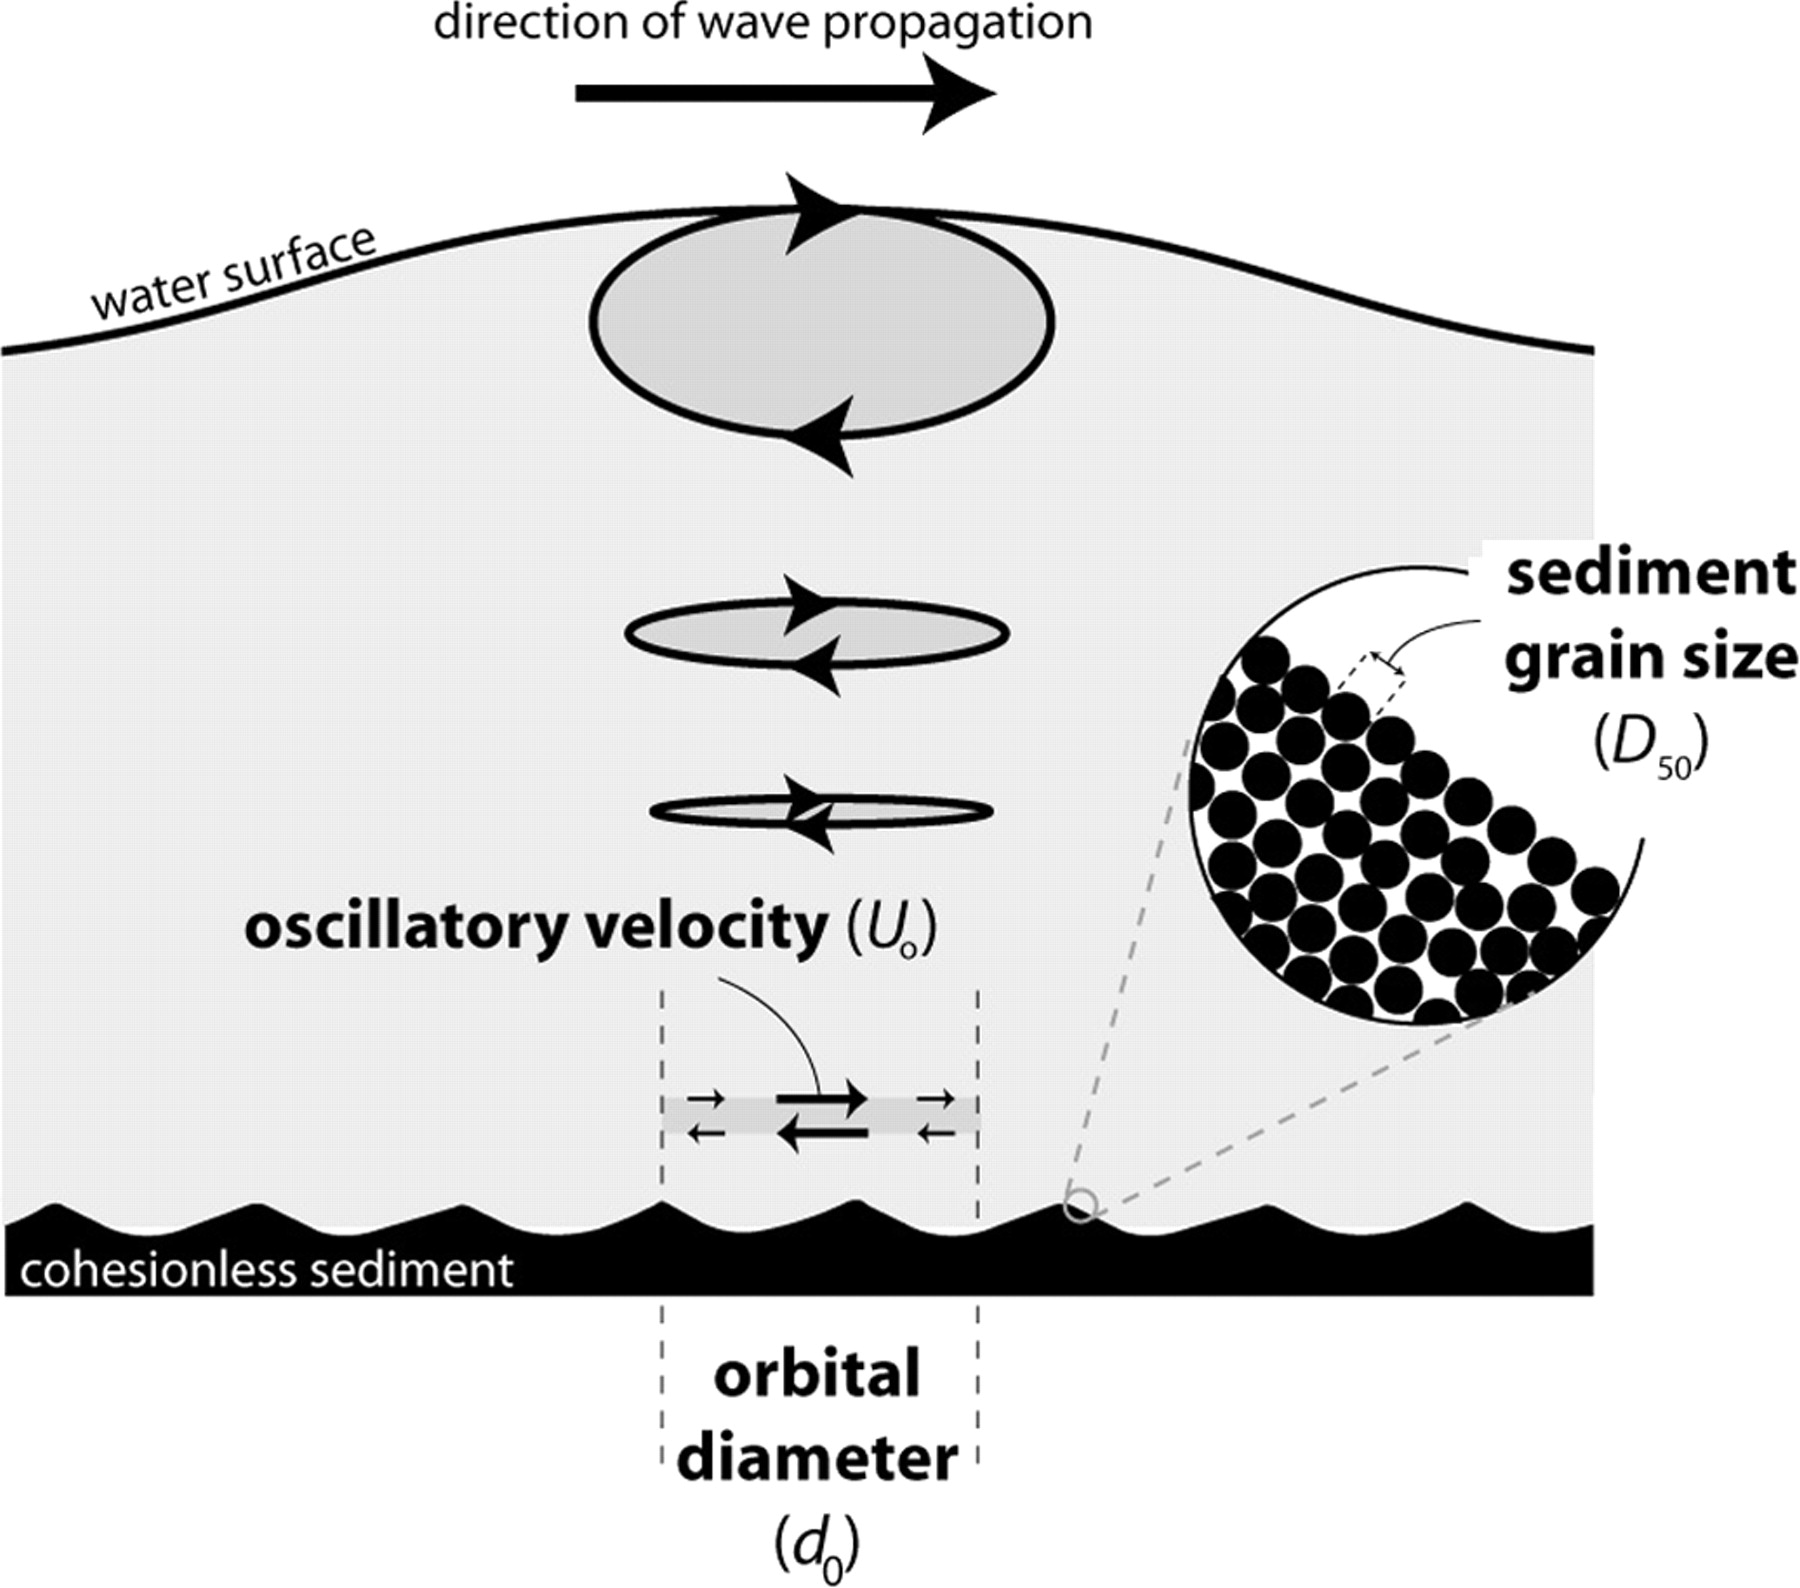
\includegraphics[scale=0.12]{./graphics/orbital_large.jpg}
\end{tabular}
\end{center}
\end{figure}

As in \textsc{Sisyphe}, the bottom shear stress due to the effect of waves and by the combined action of currents and waves are computed according to~\cite{Swart1976} and~\cite{soulsby1997dynamics}, respectively.

In \gaia, the computation of the maximum wave orbital velocity $U_w$ can be performed according to the waves characteristics: ($i$) regular (monochromatic) or ($ii$) irregular (JONSWAP spectrum)~\cite{soulsby1986direct} cases. The latter method calculates the r.m.s. orbital velocity $U_{rms}$ and then converts it to a monochromatic orbital velocity $U_w = \sqrt{2}U_{rms}$, as required by many sediment transport formulae.
Regular or irregular waves can be selected through the keyword \telkey{TYPE OF
WAVES} (integer type, set to \texttt{= 2} by default). In case of internal
coupling with \tomawac, option 2 must be used.


%-------------------------------------------------------------------------------
\subsection{Procedure for internal coupling waves-currents and sediment transport}
%-------------------------------------------------------------------------------
The internal coupling between waves-currents and sediment transport is implemented in the \telemacsystem{}, requiring the set of input files (steering file, geometry file, etc.) for the modules \telemac{2D}, \tomawac{} and \gaia{}:
\begin{itemize}
  \item \telemac{2D} steering file:
\begin{itemize}
\item The keyword {\ttfamily COUPLING WITH = 'TOMAWAC, GAIA'} activates the internal coupling with modules \tomawac{} and \gaia{}
\item The keyword {\ttfamily WAVE DRIVEN CURRENTS = YES} (real type, set to \texttt{= NO} by default) allows to incorporate the influence of \textit{radiation stresses} in the mean flow (wave-induced currents), computed by the subroutine {\ttfamily radiat.f} (\tomawac{}).
\end{itemize}

 \item \gaia{} steering file:
\begin{itemize}
\item The keyword {\ttfamily EFFECT OF WAVES} (logical type, set to {\ttfamily = NO} by default) is used to consider the effect of the waves on the solid transport formula
\item The keyword {\ttfamily BED-LOAD TRANSPORT FORMULA FOR ALL SANDS} (integer type variable, {\ttfamily = 1} by default) allows to choose among the transport formulas that consider the combined effect of currents and waves:
\begin{lstlisting}[frame=trBL]
4 : BIJKER
5 : SOULSBY - VAN RIJN
8 : BAILARD
9 : DIBAJNIA ET WATANABE
\end{lstlisting}
\end{itemize}
\end{itemize}

%-------------------------------------------------------------------------------
\subsection{Time steps and coupling period considerations}
%-------------------------------------------------------------------------------
We call $\Delta t_{T2D}, \Delta t_{GAI}, \Delta t_{TOM}$ respectively the time steps for hydrodynamics (computed by \telemac{2D}), sediment transport (computed by \gaia{}) and waves (computed by \tomawac{}). We define $CP_{T2D-GAI}$ the coupling period for \telemac{2D} and \gaia{} and $CP_{T2D-TOM}$ the coupling period for \telemac{2D} and \tomawac{}. The morphological time step is $\rightarrow \Delta t_{T2D} \times CP_{T2D-GAI}$.


In the subroutine {\ttfamily wac.F} of \tomawac{}, the following restrictions are verified:
\begin{itemize}
\item[(1)] Check for multiplicity between $\Delta t_{TOM}$ and $\Delta t_{T2D}$:
\begin{equation*}
\left|\parallel\frac{\Delta t^{\max}}{\Delta t^{\min}}\parallel-\frac{\Delta t^{\max}}{\Delta t^{\min}}\right|>\varepsilon %\left| \right|
\end{equation*}
$\Delta t^{\max}=\max{(\Delta t_{TOM}, \Delta t_{T2D} \times CP_{T2D-TOM})}$, $\Delta t^{\min}=\min{(\Delta t_{TOM}, \Delta t_{T2D} \times CP_{T2D-TOM})}$, \\
$\parallel\cdot\parallel=$\texttt{NINT(A)} rounds its argument to the nearest whole number
\item[(2)] Check $\Delta t_{TOM} \leq \Delta t_{T2D} \times CP_{T2D-TOM}$
\end{itemize}

\begin{figure}[H]%
  \begin{center}
    \begin{tabular}{c}
      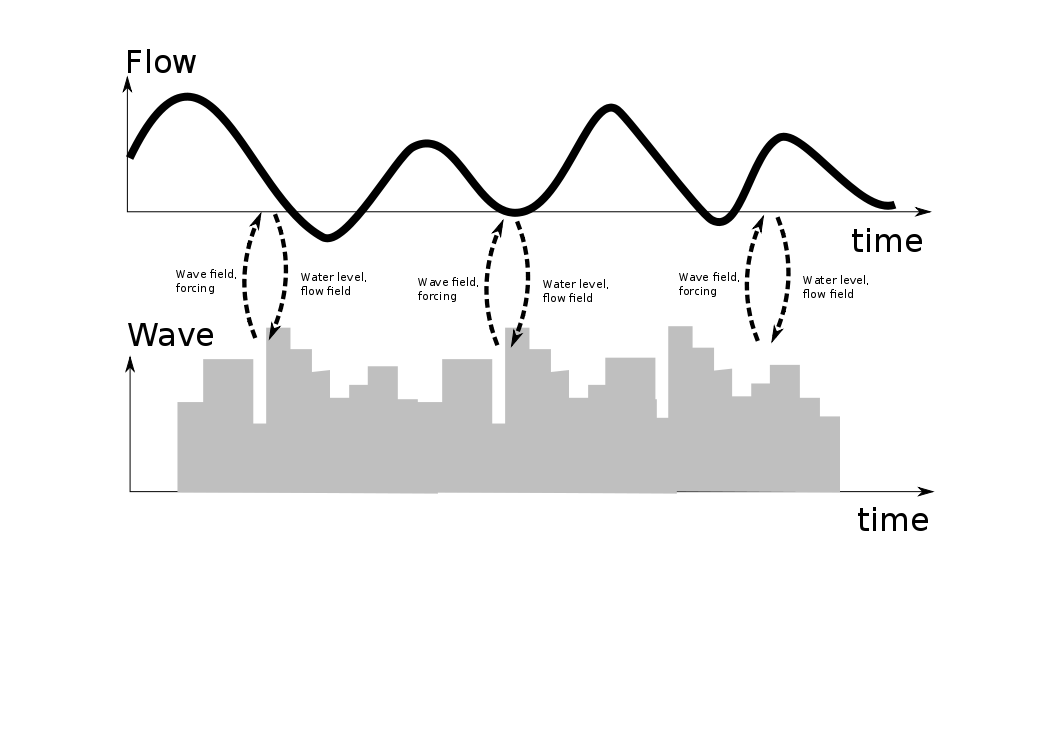
\includegraphics[scale=0.30]{./graphics/coupling_1.png}
\end{tabular}
\end{center}
\end{figure}

\begin{figure}[H]%
  \begin{center}
    \begin{tabular}{c}
      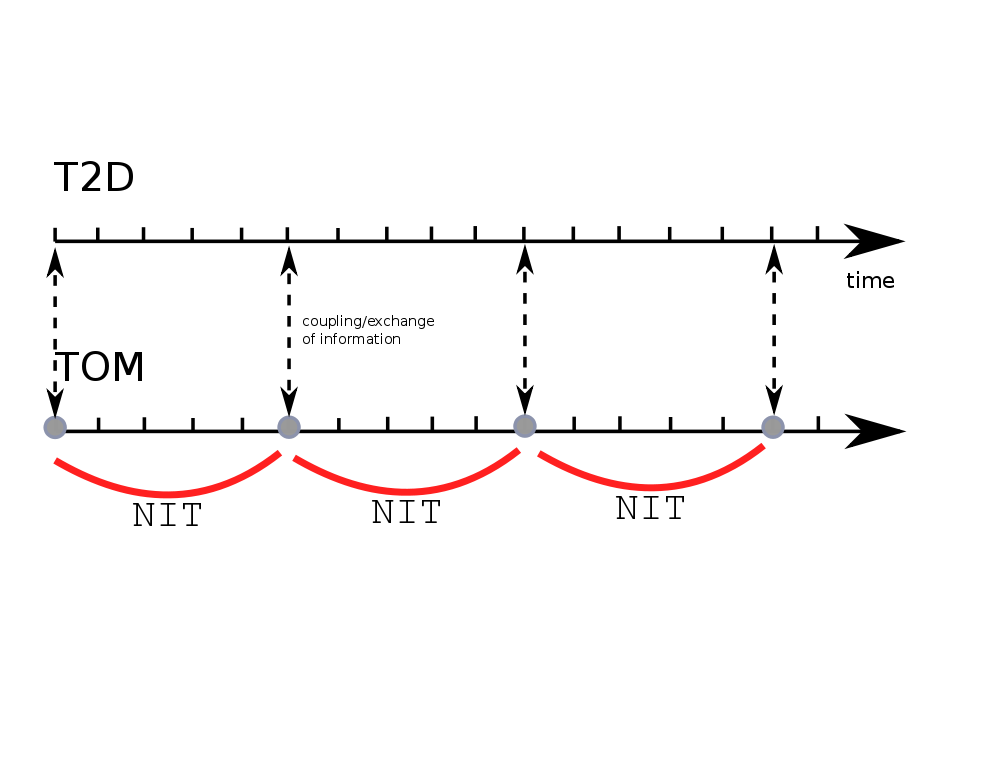
\includegraphics[scale=0.30]{./graphics/coupling_2.png}
    \end{tabular}
    \caption{Example for $\Delta t_{T2D}=1$~s, $\Delta t_{TOM}=1$~s, $CP_{T2D-TOM}=5$ ($NIT=\Delta t_{T2D}\times CP_{T2D-TOM}/\Delta t_{TOM}$)}
\end{center}
\end{figure}


%-------------------------------------------------------------------------------
\subsection{Wave orbital velocity}
%-------------------------------------------------------------------------------
The wave orbital velocity $U_w$ is computed assuming the validity of the linear theory:
\begin{equation*}
U_w=\frac{H_s \omega }{2 \sinh (kh)},
\end{equation*}
where $h$ is the water depth, $\omega = 2\pi/T_p$ is the intrinsic angular frequency, $k = 2\pi/L$ is the wave number, with $L$ the wave length. The wave number is calculated from the dispersion relation:
\begin{equation*}
\omega^2 = gk\tanh (kh).
\end{equation*}
This variable ({\ttfamily UWBM}) is computed by \tomawac{} in the subroutine {\ttfamily vitfon.f}.

%-------------------------------------------------------------------------------
\subsection{Wave-induced bottom friction}
%-------------------------------------------------------------------------------
The maximum stress due to waves is calculated at each time step as a
function of the wave-orbital velocity $U_w$ by use of a quadratic
friction coefficient $f_w$ due to waves:
\begin{equation*}
  \tau_w = \frac{1}{2}\rho f_w U_w^2.
\end{equation*}
The wave friction factor $f_w$ is calculated as a function of relative
density:
\begin{equation*}
f_w = f_w \left( A_0/k_s \right),
\end{equation*}
where $A_0= U_w/\omega$ is the semi-orbital excursion and $k_s$ the bed
roughness.
In \gaia{}, the expression proposed by Swart~\cite{Swart},\cite{Swart1976} is
implemented in (\texttt{tobw\_gaia.f}):
\begin{equation*}
f_w = \max\left[ \exp \left(-5.977 + 5.213\left( \frac{A_0}{k_s} \right)^{-0.194}
 \right), 0.30 \right]
\end{equation*}

%-------------------------------------------------------------------------------
\subsection{Wave-current interactions}
%-------------------------------------------------------------------------------
For combined waves and currents, the wave-induced bottom
stresses are, in many cases, of an order of magnitude larger than in the case of currents
alone. Different models can be found in the literature to calculate the wave
and current bottom stresses $\tau_{cw}$, as a function of the bottom
shear stress due to currents only $\tau_c$ and the maximum shear
stress due to waves only $\tau_w$. Following Bijker~\cite{Bijker}:
\begin{equation}\label{eq:tauBijker}
\tau_{cw} = \tau_c + \frac{1}{2} \tau_w.
\end{equation}
%{\tiny In non-dimensional form, $\theta_c=\tau_c/\rho$, $\theta_w=\tau_w/\rho$}
See e.g. the soubroutine \texttt{bedload\_bijker.f}.

%-------------------------------------------------------------------------------
\subsection{Wave-induced sediment transport formulas}
%-------------------------------------------------------------------------------
The choice of the transport formula is done with the keyword {\ttfamily BED-LOAD TRANSPORT FORMULA FOR ALL SANDS} (integer type variable, set to {\ttfamily = 1} by default). Available formulas in \gaia{} accounting for the effect of waves superimposed to currents:
\begin{lstlisting}[frame=trBL]
4 : BIJKER
5 : SOULSBY - VAN RIJN
8 : BAILARD
9 : DIBAJNIA ET WATANABE
\end{lstlisting}

\subsubsection{Soulsby-van Rijn's formula}
\begin{itemize}
\item {\ttfamily BED-LOAD TRANSPORT FORMULA FOR ALL SANDS} \texttt{= 5}, the total transport rate due to the combined action of waves and current is computed by~\cite{Soulsby97}:
\begin{equation*}
Q_{b,s} = A_{b,s} U_c\left[ \left( U_c^2+\frac{0.018}{C_D} U_w^2\right)^{0.5}-U_{cr}\right]^{2.4}.
\end{equation*}
This formula can be applied to estimate both components of the total sand
transport rate (bedload $Q_b$ and suspension $Q_s$), and it is suitable for rippled beds (bed roughness $=6$mm)

\item The bedload and suspended load coefficients, $A_{b,s}$ are computed:
\begin{equation*}
A_b = \frac{0.005 h \left(d_{50}/h\right)^{1.2}}{\left((s-1)gd_{50}\right)^{1.2}}, \quad A_s = \frac{0.012 d_{50}D_*^{-0.6}}{\left((s-1)gd_{50}\right)^{1.2}},
\end{equation*}
where $U_c$ is the norm of the depth-averaged current velocity, $U_w$ is the orbital velocity of waves, and $C_D$ is the quadratic drag coefficient due to current alone.
\item The critical entrainment velocity $U_{cr}$ is given by:
\begin{equation*}
U_{cr} = \left\{\begin{array}{ll}
\displaystyle
0.19 d_{50}^{0.1}\log_{10}\left(\frac{4h}{d_{90}}\right), & \quad \text{if } d_{50} < 0.0005~\text{m} \\
\displaystyle
8.5 d_{50}^{0.6} \log_{10}\left(\frac{4h}{d_{90}} \right), & \quad \text{otherwise}.
\end{array}
\right.
\end{equation*}
\item The diameter $d_{90}$, characteristic of the coarser grains, can be
specified with the keyword \telkey{D90 SAND DIAMETER FOR ONLY ONE CLASS}
(real type, default value {\ttfamily = 0.01}). If several classes of
non-cohesive sediments are present, $d_{90}$ will be considered as the ratio
between the skin friction and the mean diameter $d_{50}$.
%The validity range for the Soulsby-van Rijn formula is $h = 1-20$ m, $U = 0.5-5$ms$^{-1}$, and $d_{50}=0.1-2$mm.
\item Fortran file \texttt{bedload\_soulsby.f}
\end{itemize}


\subsubsection{Bijker's formula}
\begin{itemize}
\item {\ttfamily BED-LOAD TRANSPORT FORMULA FOR ALL SANDS} \texttt{= 4}, the Bijker's formula can be used for determining the total transport rate~\cite{Bijker}. The bedload transport rate is:
\begin{equation*}
Q_b = b\,d_{50}\sqrt{\tau_c/\rho}\exp\left(-0.27\frac{(\rho_s-\rho)gd_{50}}{\mu \tau_{cw}}\right),
\end{equation*}
where $\tau_c$ is the shear stress due to currents alone, $\tau_{cw}$ the shear stress due to wave-current
interaction, and $\mu$ is a correction factor which accounts for the effect of ripples. The shear stress under combined wave and current is calculated
by Equation (\ref{eq:tauBijker}).
\item By default, in \gaia{} $b=2$ but this value can be modified with the keyword {\ttfamily B VALUE FOR THE BIJKER FORMULA} (real type, set to {\ttfamily = 2.0} by default)

\item The ripple factor correction $\mu$ is calculated in the same way as for currents only
  \item For the suspended load transport, the
concentration profile is assumed to be in equilibrium.

\item After depth-integration and by assuming a Rouse profile for the concentration
and a logarithmic velocity profile for the mean velocity profile, the
suspended load can be written as:
\begin{equation*}
Q_{s} = Q_{b} I,
\end{equation*}
where
\begin{equation*}
I=1.83\times 0.216\frac{B^{A-1}}{(1-B)^A} \int_B^1
\left(\frac{1-y}{y}\right)^A \ln\left(\frac{33y}{B}\right) d y,
\end{equation*}
with
\begin{equation*}
A = \frac{w_s}{\kappa u_*},\quad u_*=\sqrt{\frac{\tau_{cw}}{\rho}},\quad B = k_s/h.
\end{equation*}
\item Fortran file \texttt{bedload\_bijker.f}
\end{itemize}

Details of Bailard and Dibajnia and Watanabe wave-induced sediment transport formulas can be found in~\cite{Bailard} and \cite{Dibajnia}, respectively.


%-------------------------------------------------------------------------------
\subsection{Steering file setup for sediment transport including waves effects}
%-------------------------------------------------------------------------------
In \gaia{}, the effect of waves can be incorporated into the numerical simulation when the keyword
 {\ttfamily EFFECT OF WAVES} (logical type, set to {\ttfamily = NO} by default) is activated.

 To compute sediment transport rates due to the action of waves, the spectral significant wave height ($H_s =$, variable \texttt{HM0}), the wave peak period ($T_p =$, variable \texttt{TPR5}) and the mean wave direction ($\theta_w =$, variable \texttt{DMOY}, relative to the $x-$axis) need to be specified.

 \begin{itemize}
\item Spectral significant wave height ($H_s =$ \texttt{HM0}): $H_s=4\sqrt{m_0}$, with $m_0$ the momentum of order $0$ of the wave spectrum (variance of the sea state) [m]
\vspace{0.2cm}
\item Wave peak period ($T_p =$ \texttt{TPR5}): peak period computed by the Read's method of order $5$ [s]
\vspace{0.2cm}
\item Mean wave direction ($\theta_w =$ \texttt{DMOY}, relative to the $x-$axis) [deg.]
\end{itemize}

 This information can be provided from a Fortran file (subroutine \texttt{user\_forcing.f}) which reads a file containing those variables previously computed by the wave module (e.g. \tomawac{}), or by internal coupling with the wave module.
%-------------------------------------------------------------------------------
\subsection{Procedure for external coupling waves-currents and sediment transport}
%-------------------------------------------------------------------------------
\begin{itemize}
\item A \telemac{2D} $+$ \tomawac{} simulation (same mesh) is launched and the spectral significant wave height ($H_s =$ \texttt{HM0}), the wave period ($T_p =$ \texttt{TPR5}) and the mean wave direction ($\theta_w =$ \texttt{DMOY}) are recorded in the \tomawac{}'s result file (format selafin). The mean wave direction can be recorded following the nautical or the trigonometrical convention (with respect to the $x-$axis), according to the keyword \telkey{TRIGONOMETRICAL CONVENTION} set in the \tomawac{} steering file (see the \tomawac{} user manual for more details).

\item In \telemac{2D} steering file, the keyword {\ttfamily WAVE DRIVEN CURRENTS} (logical type, set to {\ttfamily = NO} by default) allows to incorporate the influence of radiation stresses in the mean flow (wave-induced currents)

\item The external coupling between waves-currents and sediment transport requires the set of input files (steering, geometry, etc.) for the modules \telemac{2D} and \gaia{} and a results file \tomawac{}



\end{itemize}

\begin{itemize}
\item \telemac{2D} steering file:
\begin{itemize}
\item The keyword {\ttfamily COUPLING WITH = 'GAIA'} activates the internal coupling with module \gaia{}
\item The keyword {\ttfamily BINARY DATA FILE 1} is used to open the \tomawac{} results file
\item A Fortran file containing the subroutine \texttt{prosou.f} allows to read non-stationary wave data from a binary result file produced on the same mesh by \tomawac{}
\end{itemize}
\item \gaia{} steering file:
\begin{itemize}
\item The keyword {\ttfamily EFFECT OF WAVES} (logical type, set to {\ttfamily = NO} by default) is used to consider the effect of the waves on the solid transport formula
\item The keyword {\ttfamily BED-LOAD TRANSPORT FORMULA FOR ALL SANDS} (integer type variable, {\ttfamily = 1} by default) allows to choose among the transport formulas that consider the combined effect of currents and waves
\item The keyword {\ttfamily TRIGONOMETRICAL CONVENTION IN WAVE FILE} (logical type variable, {\ttfamily = NO} by default) allows to consider the convention (nautical or trigonometrical) used in \tomawac{}'s result file for wave direction. This keyword is necessary when there is no internal coupling between \gaia{} and \tomawac{} (i.e. the \tomawac{}'s result file is generated separately by a \telemac{2D} $+$ \tomawac{} simulation).
\end{itemize}
\end{itemize}

\begin{itemize}
\item In \telemac{2D}, the keyword {\ttfamily NAMES OF CLANDESTINE VARIABLES} names the variables that belong to the other code and are given back in the results file:
\begin{lstlisting}[frame=trBL]
NAMES OF CLANDESTINE VARIABLES=
'WAVE HEIGHT HM0 M               ';
'PEAK PERIOD TPR5S               ';
'MEAN DIRECTION  DEG             '
\end{lstlisting}
\end{itemize}

%-------------------------------------------------------------------------------
\subsection{Useful graphical printouts}
%-------------------------------------------------------------------------------
Keyword {\ttfamily VARIABLES FOR GRAPHIC PRINTOUTS}:
\begin{lstlisting}[frame=trBL]
THETAW="wave angle with axis Oy (deg)";
W="wave height";
X="wave period";
UWB="wave orbital velocity (m/s)";
TOB="bed shear stress(N/m2)";
MU ="skin friction coefficient";
N="bed-load discharge along x axis (m2/s)";
P="bed-load discharge along y axis (m2/s)";
E="bottom evolution (m)";
QSBL="bed load transport rate (m2/s)";
\end{lstlisting}


%----------------------------------------------------------------------------------------
%	CHAPTER 6: How-To?
%----------------------------------------------------------------------------------------

%-------------------------------------------------------------------------------
\chapter[How-To?]{How-To?}
\label{chap:how-to}
%-------------------------------------------------------------------------------
\pagebreak
%...............................................................................
\section{Running a morphodynamics simulation: first steps}
%...............................................................................
The minimum set of files to run a morphodynamics simulation includes:
\begin{itemize}
\item the steering file(s) (text/ASCII file \texttt{*.cas})
\item the geometry file (format selafin/binary \texttt{*.slf})
\item the boundary conditions file (text/ASCII file \texttt{*.cli})
\item additional or optional input files as the Fortran file (text/ASCII file \texttt{*.f}), the reference file (format selafin/binary \texttt{*.slf}), etc.
\end{itemize}

Typically, these files are contained in a folder, for example in the folder simulation:
\begin{footnotesize}
\begin{verbatim}
simulation\bc_bifurcation_tel.cli
simulation\geo_bifurcation.slf
simulation\res_bifurcation_hotstart_tel.slf
simulation\run_bifurcation_gai.cas
simulation\run_bifurcation_tel.cas
\end{verbatim}
\end{footnotesize}
Running a simulation from a Linux terminal:
\begin{footnotesize}
\begin{verbatim}
telemac2d.py run_bifurcation_tel.cas
\end{verbatim}
\end{footnotesize}

%...............................................................................
\subsection{\gaia{}'s steering file (\texttt{*.cas})}
%...............................................................................
This file contains the necessary information for running a simulation, it also must include the values of parameters that are different from the default values (as specified in the dictionary file \texttt{gaia.dico}):
\begin{itemize}
\item Input and output files
\item Physical parameters (sand diameter, settling velocity, etc.)
\item Main sediment transport processes (transport mechanisms, closure relationships, etc.)
\item Additional sediment transport processes (secondary currents, slope effect, etc.)
\item Numerical options and parameters (numerical scheme, solvers, etc.)
\end{itemize}

\pagebreak

%-------------------------------------------------------------------------------
\subsubsection{Sketch of the gaia's steering file (\texttt{*.cas})}
%-------------------------------------------------------------------------------
\lstset{language=TelemacCas,
        basicstyle=\scriptsize\ttfamily}
\begin{lstlisting}[frame=trBL]
/----------------------------------------------------------------------/
/ gaia bedload                                                      /
/----------------------------------------------------------------------/
/
/----------------------------------------------------------------------/
/  FILES                                                               /
/----------------------------------------------------------------------/
/
/ --- GEOMETRY ---
GEOMETRY FILE				= '../geo_bifurcation.slf'
BOUNDARY CONDITIONS FILE		= '../bc_bifurcation_tel.cli'
/
/ --- RESULTS ---
RESULTS FILE				= 'res_bifurcation_gai.slf'
/
...
/----------------------------------------------
/  PHYSICAL PARAMETERS
/----------------------------------------------
/
BED LOAD FOR ALL SANDS                     = YES
BED-LOAD TRANSPORT FORMULA FOR ALL SANDS   = 1
CLASSES SEDIMENT DIAMETERS                 = 0.000120
/
...
/----------------------------------------------------------------------/
/  NUMERICAL PARAMETERS                                                /
/----------------------------------------------------------------------/
/
MASS-BALANCE                              = YES
...
\end{lstlisting}

%-------------------------------------------------------------------------------
\subsubsection{Examples of physical parameters in the \gaia{}'s steering file}
%-------------------------------------------------------------------------------
\begin{itemize}
\item Sediment diameters, defined by the keyword \telkey{CLASSES SEDIMENT DIAMETERS} (real list, {\ttfamily = 0.01} m by default)
\item Sediment density, defined by the keyword \telkey{CLASSES SEDIMENT DENSITY} (real type, {\ttfamily = 2650.0} kg$/$m$^3$ by default)
\item Critical Shields parameter, $\theta_{cr}$ ($-$), defined by the keyword \telkey{CLASSES SHIELDS PARAMETERS} (real list, = -9 by default). If it is not known, it is necessary to give a negative value to let \gaia{} compute it as a function of the non-dimensional grain diameter $D_*=d_{50}[(\rho_s/\rho-1)g/\nu^2]^{1/3}$ in the subroutine \texttt{shields.f}:
\begin{equation*}
\frac{\tau_c}{g(\rho_s -\rho)d_{50}}=\left\{\begin{array}{ll}
0.24 D_*^{-1}, & D_* \leq 4 \\
0.14 D_*^{-0.64}, & 4 < D_* \leq 10 \\
 0.04 D_*^{-0.10}, & 10 < D_* \leq 20\\
0.013 D_*^{0.29}, & 20 < D_* \leq 150 \\
0.045, & 150 \leq D_*
\end{array}
\right.
\end{equation*}
with $d_{50}$ the median sand grain diameter (m), $\rho$ the water density =1000~kg/m$^3$ by default
in \telemac{2D} and =1025~kg/m$^3$, $\rho_s$ the sediment density =2650~kg/m$^3$ by default, and $\nu$ the kinematic viscosity $=1.0\times 10^{-6}$m$^2$s$^{-1}$ by default.

\item Settling velocity, it can be specified by the user or calculated by the model as a function of grain diameter, keyword \telkey{CLASSES SETTLING VELOCITIES} (real list, =-9 by default). If a negative value is given, \gaia{} will compute it as function of grain diameter (cf. chapter \ref{Chap:Sed:Ex:cohesive}):
  \begin{equation*}
w_{s} = \left\{\begin{array}{ll}
\displaystyle
\frac{(s-1)g d_{50}^2}{18\nu}, & \quad \text{if } d_{50} \leq 10^{-4} \\
\displaystyle
\frac{10\nu}{d_{50}} \left(\sqrt{1+0.01\frac{(s-1)gd_{50}^3}{\nu^2}}-1\right), & \quad \text{if } 10^{-4} \leq d_{50} \leq 10^{-3}\\
\displaystyle
1.1 \sqrt{(s-1)gd_{50}}, & \quad \text{otherwise}
\end{array}
\right.
\end{equation*}
with $s=\rho_{s}/\rho$ is the relative density and $g$ is the acceleration of the gravity.%
\item Bed porosity, keyword \telkey{LAYERS NON COHESIVE BED POROSITY} (real type, {\ttfamily = 0.40} by default)
\end{itemize}



\subsection{Boundary conditions file}\label{sec:flags}
Thirteen variables for each boundary nodes are specified in the boundary condition file (usually named with extension \texttt{*.cli}). An example is given below:

\begin{lstlisting}[frame=trBL]
5 4 4 0.0 0.0 0.0 0.0 4 0.0 0.0 0.0 565 1
5 4 4 0.0 0.0 0.0 0.0 4 0.0 0.0 0.0 564 2
5 4 4 0.0 0.0 0.0 0.0 4 0.0 0.0 0.0 563 3
5 4 4 0.0 0.0 0.0 0.0 4 0.0 0.0 0.0 562 4
5 4 4 0.0 0.0 0.0 0.0 4 0.0 0.0 0.0 561 5
5 4 4 0.0 0.0 0.0 0.0 4 0.0 0.0 0.0 560 6
\end{lstlisting}

Each column is named after a flag, as follows:
\subsubsection{\telemac{2D}}
\begin{lstlisting}[frame=trBL]
LIHBOR LIUBOR LIVBOR HBOR UBOR VBOR AUBOR LITBOR TBOR ATBOR BTBOR N K
\end{lstlisting}
\subsubsection{\gaia{}}
\begin{lstlisting}[frame=trBL]
LIHBOR LIQBOR LIVBOR Q2BOR UBOR VBOR AUBOR LIEBOR/LICBOR EBOR/CBOR ATBOR BTBOR N K
\end{lstlisting}
%\begin{center}
%\begin{small}
%\texttt{\textcolor{black}{LIHBOR}, \textcolor{black}{LIUBOR/LIQBOR}, \textcolor{black}{LIVBOR}, \textcolor{black}{HBOR}, \textcolor{black}{VBOR}, \textcolor{black}{UBOR}, \textcolor{black}{VBOR}, \textcolor{black}{CHBORD}, \textcolor{black}{LITBOR/LIEBOR/LICBOR}, COL10, COL11, G, L}
%\end{small}
%\end{center}
where \texttt{N, K} are respectively the global and local boundary node numeration. Flags \texttt{ATBOR, BTBOR} are discussed in the \telemac{2D} user manual. For both modules \telemac{2D} and \gaia{}, flags can be specified as follows:
\begin{itemize}
\item \texttt{\textcolor{black}{=2:}} closed boundary (wall)
\item \texttt{\textcolor{black}{=4:}} free boundary (Neumann's type)
\item \texttt{\textcolor{black}{=5,6:}} imposed value (Dirichlet's type)
\end{itemize}

The different types of boundaries are (integer variables):
\subsubsection{\telemac{2D}}
\begin{itemize}
\item \texttt{\textcolor{black}{LIHBOR:}} flag to set the water depth (\texttt{=5})
\item \texttt{\textcolor{black}{LIUBOR:}} flag to set the discharge (\texttt{=5}) or the velocity (\texttt{=6}) in the $x-$direction
\item \texttt{\textcolor{black}{LIVBOR:}} flag to set the discharge (\texttt{=5}) or the velocity (\texttt{=6}) in the $y-$direction
\item \texttt{\textcolor{black}{LITBOR:}} flag to set the tracer
\end{itemize}
For further details see the \telemac{2D}'s or \telemac{3D} user manual.
\subsubsection{\gaia{}}
\begin{itemize}
\item \texttt{\textcolor{black}{LIEBOR:}} flag to set the bottom elevation
\item \texttt{\textcolor{black}{LICBOR:}} flag to set the equilibrium or imposed concentration
  \item \texttt{\textcolor{black}{LIQBOR:}} flag to set the imposed bedload discharge
\end{itemize}

Values (real variables) can be specified as follows:
\subsubsection{\telemac{2D}}
\begin{itemize}
\item \texttt{\textcolor{black}{HBOR:}} prescribed water depth
\item \texttt{\textcolor{black}{UBOR:}} prescribed discharge or velocity in the $x-$direction
\item \texttt{\textcolor{black}{VBOR:}} prescribed discharge or velocity in the $y-$direction
\item \texttt{\textcolor{black}{AUBOR:}} friction coefficient on lateral walls
\end{itemize}
\subsubsection{\gaia{}}
\begin{itemize}
\item \texttt{\textcolor{black}{EBOR:}} prescribed bed evolution
\item \texttt{\textcolor{black}{CBOR:}} prescribed concentration
\item \texttt{\textcolor{black}{Q2BOR:}} prescribed bedload discharge, expressed in kg/(m~s).
\end{itemize}

For the particular case where a bedload solid discharge is imposed, an extra boundary condition file needs to be defined for \gaia{}. The treatment of boundary conditions for bedload and suspended sediment transport is given in \S\ref{sec:BedloadTransport} and \S\ref{chap:SuspendedSedimentTransport}, respectively.

%...............................................................................
\subsubsection{Coupling hydrodynamics and morphodynamics: sketch of the Telemac-2d's steering file with the required keywords}
%...............................................................................
\lstset{language=TelemacCas,
        basicstyle=\scriptsize\ttfamily}
\begin{lstlisting}[frame=trBL]
...
INITIAL TIME SET TO ZERO                = YES
TIME STEP			        = 20.0
NUMBER OF TIME STEPS                    = 100000
...
/----------------------------------------------------------------------/
/  COUPLING WITH GAIA                                                  /
/----------------------------------------------------------------------/
/
COUPLING WITH                            = 'GAIA'
GAIA STEERING FILE                    = 'run_bifurcation_gai.cas'
/
/---------------------------------------------------------------------
/ INITIAL CONDITIONS
/---------------------------------------------------------------------
/
COMPUTATION CONTINUED             = YES
PREVIOUS COMPUTATION FILE         = 'res_bifurcation_hotstart_tel.slf'
...
\end{lstlisting}
%...............................................................................
\subsection{Fortran files (\texttt{*.f})}
%...............................................................................
Programming can be necessary for particular applications. A Fortran file (keyword \telkey{FORTRAN FILE}) can be specified in the \telemac{2D} or \telemac{3D} or \gaia steering file with the required subroutine(s). All subroutines (\gaia subroutines also) can be incorporated in the \telemac{} Fortran file. Is is also possible to have a \telemac and a \gaia Fortran file. Be aware, if there is no \telemac{2D} or \telemac{3D} Fortran file, the \gaia Fortran file will not taken into account.
Some common applications are given below:
\begin{itemize}
\item \textbf{Definition of rigid areas:} \texttt{user\_bed\_init.f} is used for specifying the rigid areas. The thickness of the erodable area (array \texttt{ESTRATUM}) is imposed in this subroutine

\item \textbf{New sediment transport formula}: \texttt{user\_bedload\_qb.f} can be used to program a sediment transport formula that is different from those already implemented in \gaia{}

\item \textbf{Replace data from a result file}: \texttt{user\_forcing.f} can be used for replacing data from a results file computed from a simulation performed for example from the waves module \tomawac{}

\end{itemize}

\gaia{}'s main subroutines are found in the folder \texttt{\$HOMTEL/sources/gaia/} of the \telemacsystem{}. Please note that if there is no Fortran file specified in \telemac{2D} or \telemac{3D}, then \gaia's Fortran file must be specified in the \telemac{2D} or \telemac{3D} steering file.

\pagebreak

%-------------------------------------------------------------------------------
\subsubsection{Graphical printouts}
%-------------------------------------------------------------------------------
The keyword \telkey{VARIABLES FOR GRAPHIC PRINTOUTS} can include a variety of output variables to be printed in the results file (character list, set to {\ttfamily = U,V,H,S,B,R,E} by default). The graphic and listing printout periods are the same as in the \telemac{2D} or \telemac{3D} computation. The list of variables that can be printed in the \gaia{}'s results file can be found in the dictionary and is:
\begin{lstlisting}[frame=trBL]
U="velocity along x axis (m/s)";
V="velocity along y axis (m/s)";
H="water depth (m)";
S="free surface elevation (m)";
B="bottom elevation (m)";
Q="scalar flowrate of fluid (m2/s)";
I="flowrate along x axis (m2/s)";
J="flowrate along y axis (m2/s)";
R="non erodable bottom";
TOB="Bed Shear stress (Totalfriction) (N/m2)";
W="wave height";
X="wave period";
THETAW="wave angle with axis Oy (deg)";
M="bed-load discharge (kg/(m*s))";
N="bed-load discharge along x axis (kg/(m*s))";
P="bed-load discharge along y axis (kg/(m*s))";
E="bottom evolution (m)";
KS="total bed roughness (m)";
MU="Skin friction correction factor";
D50="Mean grain diameter";
UWB="wave orbital velocity (m/s)";
kAi="fraction of non cohesive sediment of class i, in k layer";
QSi="solid transport load of class i";
CSi="mass concentration of class i";
C2DSi="mass concentration of class i for 2D graphic printouts";
SVXi="sediment viscosity along x axis (m2/s) - only 3D";
SVYi="sediment viscosity along y axis (m2/s) - only 3D";
SVZi="sediment viscosity along z axis (m2/s) - only 3D";
QSBL="bed load transport rate (kg/(m*s))";
QSBLX="bed load transport rate x axis";
QSBLY="bed load transport rate y axis";
QSBLi="bedload transport rate of class i";
kES="thickness of the k layer";
kCONC="concentration of bed layer k";
QSi="bed load transport rate of sediment of class i";
A="supplementary variable A";
G="supplementary variable G";
L="supplementary variable L";
O="supplementary variable O";
kRi="fraction of cohesive sediment of class i, in k layer";
kSi="mass of non cohesive sediment of class i, in k layer";
kMi="mass of cohesive sediment of class i, in k layer";
ZRL="reference level for Nestor"'

\end{lstlisting}

It is worth to notice that the following variables will be printed in the hydrodynamic results file (of \telemac{2D} or \telemac{3D}) even if asked in the \gaia{} steering file:
CSi,C2DSi,SVXi,SVYi,SVZi.
The graphical printout period is controlled in the \telemac{2D} steering file through the keyword \telkey{GRAPHIC PRINTOUT PERIOD} (integer type, {\ttfamily = 1} by default).
Similarly, the keyword \telkey{LISTING PRINTOUT PERIOD} (integer type, {\ttfamily = 1} by default) controls the printout period on the screen.

%-------------------------------------------------------------------------------
\section{Compute sediment fluxes through a given section(s)}
%-------------------------------------------------------------------------------
Use the keywords {\ttfamily FLUXLINE} (logical type, set to {\ttfamily NO} by default) and {\ttfamily FLUXLINE INPUT FILE} (character type).

The format of the {\ttfamily FLUXLINE INPUT FILE} includes (see Figure~\ref{fig:fluxline_example}):
\begin{itemize}
\item The number of fluxlines (integer)
\item The definition of the fluxlines, given by:
  \begin{itemize}
  \item The specification of two points of the fluxline (\texttt{fluxline\_x1, fluxline\_y1, fluxline\_x2, fluxline\_y2}), followed by
  \item the definition of the bounding box (\texttt{box\_x1, box\_y1, box\_x2, box\_y2})
  \item An integer (value not used)
  \end{itemize}
\end{itemize}

An example of the {\ttfamily FLUXLINE INPUT FILE} is given below:

\begin{lstlisting}[frame=trBL]
5
94.0   31.2  99.0  31.2 95.0  31.0  98.0  31.6 1
94.0   42.5  99.0  42.5 96.0  42.0  98.0  43.0 1
101.0  42.5  107.0 42.5 104.0 42.0  106.0 43.0 1
101.0  31.2  107.0 31.2 104.0 31.0  106.0 31.6 1
100.0  45.0  102.0 48.0 100.0 46.0  102.0 47.5 1
\end{lstlisting}

\begin{figure}[H]
\begin{center}
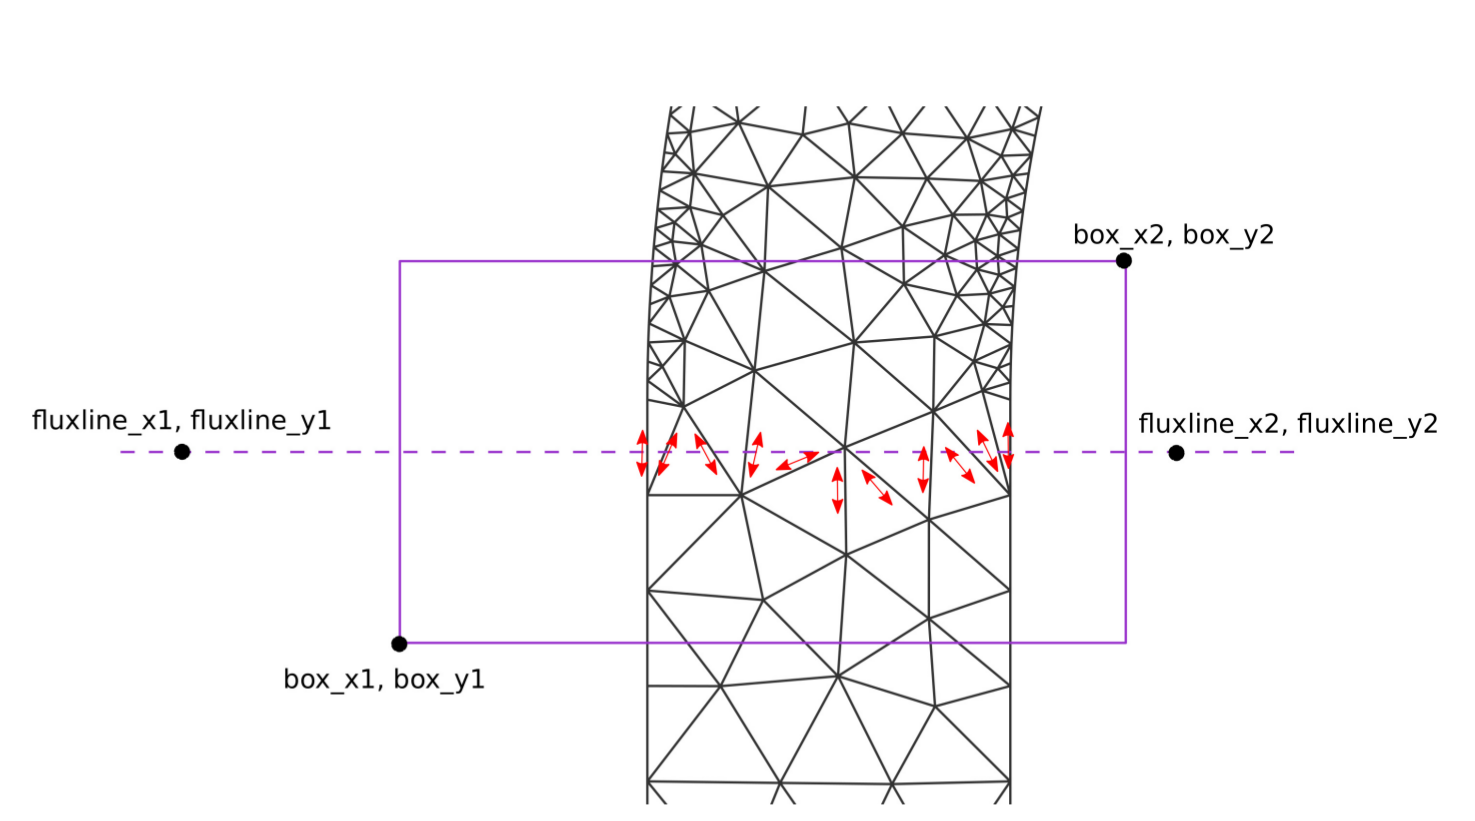
\includegraphics[scale=0.25,angle=0]{graphics/fluxline_example.png}
\caption{Description of a single fluxline and edge fluxes (red).}\label{fig:fluxline_example}
\end{center}
\end{figure}

Further details can be found in Stadler L. (2015) \textit{Calculating correct water and sediment fluxes in TELEMAC2D and SISYPHE}. Proceedings of the 22$^{nd}$
Telemac \& Mascaret User Club, STFC Daresbury Laboratory, UK, 13-16 October.

%\pagebreak
%-------------------------------------------------------------------------------
\section{Implement a new bedload transport formula}
%-------------------------------------------------------------------------------
To implement a new bedload transport formula, the keyword {\ttfamily BED-LOAD TRANSPORT FORMULA FOR ALL SANDS} must be set to {\ttfamily = 0}. The Fortran subroutine must be added into the Fortran file of \textsc{Telemac-2d} or \textsc{Telemac-3d}, keyword {\ttfamily FORTRAN FILE}.

The template subroutine is called \texttt{user\_bedload\_qb.f} and can be found in the folder \texttt{\$HOMETEL/sources/gaia}
\begin{lstlisting}[frame=trBL]
!               **************************
                SUBROUTINE USER_BEDLOAD_QB
!               **************************
     & (HN, U2D, V2D, THETAC, HOULE, HW, TW, THETAW,
     &  TOB,TOBW,TOBCW_MEAN,TOBCW_MAX, DCLA, DENS, GRAV, DSTAR, AC,
     &  XMVE, XMVS, TETAP, MU, NPOIN, QSC, QSS, CSTAEQ)
!
!***********************************************************************
! GAIA
!***********************************************************************
!
!>@brief Allows the user to code their own bedload transport
!!       formulation, best suited to their application.
!
!>@warning User subroutine; sand transport formula must be coded by the user
!>@todo Missing description of arguments
!
!~~~~~~~~~~~~~~~~~~~~~~~~~~~~~~~~~~~~~~~~~~~~~~~~~~~~~~~~~~~~~~~~~~~~~~~
!>@param[in]     HN
!>@param[in]     U2D
!>@param[in]     V2D
!>@param[in]     THETAC
!>@param[in]     HOULE
!>@param[in]     HW
!>@param[in]     TW
!>@param[in]     THETAW
!>@param[in,out] TOB
!>@param[in,out] TOBW
!>@param[in,out] TOBCW_MEAN
!>@param[in,out] TOBCW_MAX
!>@param[in]     DM
!>@param[in]     DENS
!>@param[in]     GRAV
!>@param[in]     DSTAR
!>@param[in]     AC
!>@param[in]     XMVE
!>@param[in]     XMVS
!>@param[in]     TETAP
!>@param[in]     MU
!>@param[in]     NPOIN
!>@param[in,out] QSC
!>@param[in,out] QSS
!>@param[in,out] CSTAEQ
!~~~~~~~~~~~~~~~~~~~~~~~~~~~~~~~~~~~~~~~~~~~~~~~~~~~~~~~~~~~~~~~~~~~~~~~
!
      USE INTERFACE_GAIA, EX_USER_BEDLOAD_QB => USER_BEDLOAD_QB
      USE BIEF
      USE DECLARATIONS_SPECIAL
      IMPLICIT NONE
!
!!-+-+-+-+-+-+-+-+-+-+-+-+-+-+-+-+-+-+-+-+-+-+-+-+-+-+-+-+-+-+-+-+-+-+-+
!
      TYPE(BIEF_OBJ),   INTENT(IN)    :: HN,U2D,V2D,THETAC
      TYPE(BIEF_OBJ),   INTENT(IN)    :: HW, TW, THETAW
      TYPE(BIEF_OBJ),   INTENT(IN)    :: TOB,TOBW,TOBCW_MEAN,TOBCW_MAX
      DOUBLE PRECISION, INTENT(IN)    :: DCLA, DENS, GRAV, DSTAR, AC
      DOUBLE PRECISION, INTENT(IN)    :: XMVE, XMVS
      TYPE(BIEF_OBJ),   INTENT(IN)    :: TETAP, MU
      TYPE(BIEF_OBJ),   INTENT(IN)    :: CSTAEQ
      INTEGER,          INTENT(IN)    :: NPOIN
      LOGICAL,          INTENT(IN)    :: HOULE
      TYPE(BIEF_OBJ),   INTENT(INOUT) :: QSC, QSS
!
!!-+-+-+-+-+-+-+-+-+-+-+-+-+-+-+-+-+-+-+-+-+-+-+-+-+-+-+-+-+-+-+-+-+-+-+
!
      INTEGER          :: I
!     DOUBLE PRECISION :: C1, C2, T
!
!======================================================================!
!======================================================================!
!                               PROGRAM                                !
!======================================================================!
!======================================================================!
!
!     EXAMPLE BY VAN RIJN
!
!     C1 = DENS * GRAV * DCLA
!     C2 = 0.053D0 * SQRT(DCLA**3*DENS*GRAV) * DSTAR**(-0.3D0)
!
      DO I = 1, NPOIN
!
!       TRANSPORT STAGE PARAMETER
!
!       IF(TETAP%R(I) .LE. AC) THEN
!         T = 0.D0
!       ELSE
!         T = (TETAP%R(I)-AC)/MAX(AC,1.D-06)
!       ENDIF
!
!       BEDLOAD TRANSPORT RATE
!
        QSC%R(I) = 0.D0 ! C2 * T**2.1D0
        QSS%R(I) = 0.D0
!
      ENDDO
!
!  FOLLOWING LINES NEED TO BE COMMENTED OUT
!
      WRITE(LU,53)

53    FORMAT(/,1X,'GAIA IS STOPPED : ',/
     &   ,1X,' SAND TRANSPORT MUST BE CALCULATED IN USER_BEDLOAD_QB')
      CALL PLANTE(1)
      STOP
!
!-----------------------------------------------------------------------
!
      RETURN
      END
\end{lstlisting}

%\pagebreak
%-------------------------------------------------------------------------------
%\section{Define a rigid bed}
%-------------------------------------------------------------------------------
%TODO
%\subsection{Data from selafin file}
%\subsection{Data coded by the user in the fortran file}

%\pagebreak
%-------------------------------------------------------------------------------
\section{Print a new output variable in the selafin file}
%-------------------------------------------------------------------------------
\begin{itemize}
\item Declare the {\ttfamily PRIVE} variable, for example as:

{\ttfamily USE DECLARATIONS\_GAIA, ONLY : PRIVE}

\item Use the following expression to include the variable you want to visualize:

{\ttfamily PRIVE\%ADR(N)\%P\%R(K) = [Here the variable you want to visualize]}, where {\ttfamily N} is the number of variables that you want to visualize and {\ttfamily K} is the number of nodes.

\item In the \gaia's steering file you can use the flags {\ttfamily'A'}, {\ttfamily'G'}, {\ttfamily'L'} or {\ttfamily'O'} to visualize the {\ttfamily PRIVE} variable, for example as:

{\ttfamily VARIABLES FOR GRAPHIC PRINTOUTS='U,V,S,H,B,Q,M,E,QSBL,TOB,MU,A'}
\end{itemize}

The default name {\ttfamily PRIVE 1} (for {\ttfamily N=1}) can be modified in the subroutine {\ttfamily nomvar\_gaia.f}.

\begin{lstlisting}[frame=trBL]
DO K=1, NPOIN
  PRIVE%ADR(1)%P%R(K) = [variable to visualize]
ENDDO
\end{lstlisting}

%\pagebreak
%-------------------------------------------------------------------------------
\section{Introduce a new keyword}
%-------------------------------------------------------------------------------
\begin{itemize}
\item In {\ttfamily declarations\_gaia.f} declare the variable to be called from a keyword e.g. {\ttfamily HMIN\_BEDLOAD}
\item In {\ttfamily lecdon\_gaia.f} declare .... {\ttfamily HMIN\_BEDLOAD=MOTREA(ADRESS(2,52))}
\item Declaration in the modified subroutine through {\ttfamily USE DECLARATIONS\_GAIA, ONLY : HMIN\_BEDLOAD}
\end{itemize}


%\pagebreak
%-------------------------------------------------------------------------------
% section to update
%\section{Read and use a variable from a selafin file}
%%-------------------------------------------------------------------------------
%Case of spatially distributed sediment zones
%
%\begin{itemize}
%\item Create the different zones with, e.g. BlueKenue
%\item Add in your steering file:
%  \begin{lstlisting}[frame=trBL]
%NUMBER OF PRIVATE ARRAYS = 1
%NAMES OF PRIVATE VARIABLES= 'ZONE                            '
%\end{lstlisting}
%(32 characters)%\textvisiblespace\textvisiblespace\textvisiblespace
%\item Modify the subroutine \texttt{init\_compo.f}, for example:
%\begin{lstlisting}[frame=trBL]
%      DO J=1,NPOIN
%      NCOUCHES(J)=1
%	  IF(PRIVE%ADR(1)%P%R(J).EQ.1.D0) THEN
%	  AVAIL(J,1,1)=1.D0
%	  AVAIL(J,1,2)=0.D0
%	  ELSEIF(PRIVE%ADR(1)%P%R(J).EQ.2.D0) THEN
%	  AVAIL(J,1,1)=0.D0
%	  AVAIL(J,1,2)=1.D0
%	  ELSE
%	  AVAIL(J,1,1)=0.5D0
%	  AVAIL(J,1,2)=0.5D0
%	  ENDIF
%      ENDDO
%\end{lstlisting}
%\end{itemize}


%\pagebreak
%-------------------------------------------------------------------------------
\section{Define the soil stratigraphy (\texttt{user\_bed\_init})}
%-------------------------------------------------------------------------------
In case of several layers with different sediment ratios, the subroutine \texttt{user\_bed\_init} must be used. \\
Here different layer thickness (\texttt{ESTRATUM}) and different mass ratios (\texttt{RATIO\_INIT}) for each sediment can be set.
For example for 2 layers and 4 sediments:
\begin{lstlisting}[frame=trBL]
      DO IPOIN=1,NPOIN
        ESTRATUM(1,IPOIN) = 0.12D0
        RATIO_INIT(1,1,IPOIN) = 0.5D0
        RATIO_INIT(2,1,IPOIN) = 0.5D0
        RATIO_INIT(3,1,IPOIN) = 0.D0
        RATIO_INIT(4,1,IPOIN) = 0.D0
        ESTRATUM(2,IPOIN) = 2.D0
        RATIO_INIT(1,2,IPOIN) = 0.D0
        RATIO_INIT(2,2,IPOIN) = 0.D0
        RATIO_INIT(3,2,IPOIN) = 0.5D0
        RATIO_INIT(4,2,IPOIN) = 0.5D0
      ENDDO
\end{lstlisting}

%\pagebreak
%-------------------------------------------------------------------------------
%\section{Suppress bed updating}
%-------------------------------------------------------------------------------
%Set \telkey{STATIONARY MODE = YES} (logical type, set to {\ttfamily = NO} by default)

%\pagebreak
%-------------------------------------------------------------------------------
\section{Using a non-declared variable in a \gaia{}'s subroutine}
%-------------------------------------------------------------------------------
If you want to use, for example, parameter \texttt{NPTFR} and the table \texttt{NBOR(NPTFR)} in a subroutine,
declare:

\texttt{USE DECLARATIONS\_GAIA, ONLY : NPTFR, MESH}

\texttt{INTEGER, POINTER :: NBOR(:)}

Then the following alias can be declared:

\texttt{NBOR=>MESH\%NBOR\%I}

%\pagebreak
%-------------------------------------------------------------------------------
\section{Deal with wetting and drying zones - use of
\telkey{MINIMAL VALUE OF THE WATER HEIGHT}}
%-------------------------------------------------------------------------------
At for example intertidal wetlands with flooding and drying or tidal areas, the
bottom friction could be very high when the water depth is very small, even for
small velocities, leading to high and unphysical erosion rates. To prevent that,
the keyword \telkey{MINIMAL VALUE OF THE WATER HEIGHT} can be used (real value,
by default equal to $1.0 \times 10^{-3}$m): the erosion rate will be set to zero
in nodes where h$<$h$_{min}$.
At the same time, in order to guarantee a balance between erosion and
deposition, even the deposition flux will be set to zero in the same nodes.\\
This keyword is activated when \telkey{TIDAL FLATS = YES} (default value). \\
In case of bedload, when using the keyword
\telkey{MINIMAL VALUE OF THE WATER HEIGHT},
the bedload fluxes (variable called QSC in \gaia) are also set to
zero if h$<$h$_{min}$. This is also applied when using total sediment transport
formulas (e.g. \telkey{BED-LOAD TRANSPORT FORMULA FOR ALL SANDS}
{\ttfamily= 30}). \\
Finally, the use of the keyword \telkey{MINIMAL VALUE OF THE WATER HEIGHT}
implies that the shear stress is set to zero to prevent unphysical values, if
h$<$h$_{min}$.
%@to do: describe how to use MINIMUM DEPTH FOR BEDLOAD
%\pagebreak
%-------------------------------------------------------------------------------
\section{Set a non-erodible bottom}
%-------------------------------------------------------------------------------
The non-erodible bottom (or rigid bed) can be set using the keyword \telkey{LAYERS INITIAL THICKNESS} which is equal to $100$~m by default, in case of a single layer. \\
For more complex set-up (e.g. rigid bed variable in space), the subroutine \texttt{user\_bed\_init} can be used. Here the variable \texttt{ESTRATUM} which states the thickness of the erodible bed, needs to be modify.
%\pagebreak
%-------------------------------------------------------------------------------
\section{Modify the bottom from the subroutine corfon}
%-----------------------------------------------------------------------------
For example, you want to set the bottom at node $325$ equal to $2.1$ m
\begin{itemize}
\item Sequential: \texttt{ZF\%R(325)=2.1D0}
\item Parallel: \texttt{ZF\%R(GLOBAL\_TO\_LOCAL\_POINT(325,MESH))=2.1D0}
\end{itemize}

If there are several nodes to be modified, use a loop.

{\footnotesize Thanks to JMH (post \#9747)}

%-------------------------------------------------------------------------------
\section{Dredge and dump activities}
%-------------------------------------------------------------------------------
When using the module \nestor (keyword: \telkey{NESTOR = YES}) to carry out dredge or dump activities, these files are used to
specify the action, location, geometry and the last status. The keywords identifying these files are:

\begin{enumerate}
\item  \telkey{NESTOR ACTION FILE}

\item  \telkey{NESTOR POLYGON FILE}

\item  \telkey{NESTOR SURFACE REFERENCE FILE}

\item  \telkey{NESTOR RESTART FILE}
\end{enumerate}

These files are described in detail in the \nestor User Manual.

%-------------------------------------------------------------------------------
\section{Morphological spin-up}
%-------------------------------------------------------------------------------
It is essential to start a morphological computation using fully developed hydrodynamic conditions. In an initial hydrodynamic computation, large velocities may occur, which lead to unphysical changes in the bed. There are two methods to achieve this:
\begin{enumerate}
\item Perform a separate hydrodynamic computation (without \gaia), for an initial spin up period. Use the results of this computation using the \telkey{PREVIOUS COMPUTATION FILE} in \telemac{2D} or \telemac{3D} as \textit{hotstart}.
\item Use the keyword  \telkey{SPINUP TIME FOR BED UPDATING} (real value equal to 0. by default). With this keyword, no bed level changes are taken into account during the first period of the calculation, specified with this keyword (in seconds). In this way, it is possible to perform the hydrodynamic spin-up in the morphological run, such that a second run is not needed.  In case of suspended sediment transport calculations, no bed changes due to erosion and deposition are taken into account in this period. However, the sediment concentration in the water column adapts to the hydrodynamic conditions including the erosion and deposition flux. In this way the suspended sediment concentration at the start of the morphological calculation can be in equilibrium with the hydrodynamic conditions, thus preventing rapid erosion at the initial period, typically found when starting with a water column without any suspended sediment. The keyword can thus be used for bedload, suspended load and both. An example of the use of this keyword can be found in the Yen test case.
\end{enumerate}

%-------------------------------------------------------------------------------
%\section{Set-up a graded sediment problem with only one layer}
%-----------------------------------------------------------------------------


%-------------------------------------------------------------------------------
\section{Continuing a computation}
%-------------------------------------------------------------------------------
\label{sec-restart}
Like \telemac{2D} or \telemac{3D}, \gaia enables the user to resume a
computation taking a time step
of a previous computation on the same mesh as initial state.

From v8p5, two methods are possible to continue a computation:
\begin{itemize}
\item continuing a computation using a restart file manually generated
by users from a previous computation (single solution up to v8p4),
\item continuing a computation using a restart file automatically generated
by \gaia (and \telemac{2D} or \telemac{3D}) (new method introduced in v8p5).
Advantages of this last approach are:
\begin{itemize}
  \item the result file only contains variables of interest for users
(and not variables necessary to restart, as for the first approach) which
allows files of smaller size.
In particular less variables are saved at every graphic printout
and no extra variables are needed for sediments of type CO,
  \item users do not have to think and select variables necessary for restart
as they are automatically chosen by the code during the first simulation,
  \item the restart is done without information losses for two reasons:
first, variables necessary for restart are grabbed from the restart file without
recomputing them by means of other variables;
second, the default option uses a double precision format to generate the
restart file.
The only drawback in this case is that this file is larger compared to the
single precision format.
\end{itemize}
\end{itemize}

The first approach is described here below.
By default, as for \telemac{2D} or \telemac{3D}, \gaia reads the last record of
the previous computation result file.
Using the keyword \telkey{RECORD NUMBER FOR RESTART} allows specifying
the number of the iteration to be read (default = -1 means the last record is
taken).
This keyword has been introduced in release v8.5
(before, it was only possible to continue a computation from the last record
of the \telkey{PREVIOUS SEDIMENTOLOGICAL COMPUTATION FILE}).

In this case, it is essential that the continuation file contains
all the information required by \gaia{}.
However, in some cases, the software is capable of recomputing some
variables from others provided.
If some variables are missing from the continuation file,
they are then fixed automatically at zero.

In order to use the continuation file, it is necessary to enter
two keywords in the steering file:

\begin{itemize}
\item The keyword \telkey{COMPUTATION CONTINUED} must have the value YES
(default value = NO),

\item The keyword \telkey{PREVIOUS SEDIMENTOLOGICAL COMPUTATION FILE} must
provide the name of the file that will supply the initial state.
\end{itemize}

N.B.: the mesh for which the results are computed must be exactly the same
as the one to be used in continuing the computation.

If necessary, the keyword
\telkey{PREVIOUS SEDIMENTOLOGICAL COMPUTATION FILE FORMAT}
can be used to select a specific format.
For example, in order to increase the accuracy of the initial state,
it is possible to use double precision SERAFIN format ('SERAFIND') or
MED format ('MED').
Obviously, this configuration is possible only if the previous computation
was correctly configured in terms of results file format.
\\

The second approach is described here below.
Resuming the computation usually leads to small differences in results
compared to the same calculation without interruption.
To correct this, the user has a specific recovery procedure
to improve the accuracy of calculations, using double precision format SERAFIN
files (or MED format) for the keyword \telkey{RESTART FILE FORMAT}
(default = SERAFIND):

\begin{itemize}
\item In the first computation, the keyword \telkey{RESTART MODE} is set to
YES (default = NO),
which generates a specific file containing the full information at one or a
few time step(s) of the simulation.
The name of this file is given by the keyword \telkey{RESTART FILE},

\item In the second computation, this specific file must be used as
\telkey{PREVIOUS SEDIMENTOLOGICAL COMPUTATION FILE} specifying the
\telkey{PREVIOUS SEDIMENTOLOGICAL COMPUTATION FILE FORMAT} is 'SERAFIND'
(SERAFIN double precision).
If the restart should be done from the last time step saved in the
\telkey{RESTART FILE}, the keyword \telkey{RECORD NUMBER FOR RESTART} is to be
let to default value (= -1), otherwise it should be changed.
\end{itemize}

In the first computation, there are 2 keywords which can enable to tune the
resuming of the computation:
\begin{itemize}
\item If wanting to generate a \telkey{RESTART FILE} at a specific number of
time step different from the last one, the keyword
\telkey{RECORD NUMBER IN RESTART FILE} is to be used
(default = -1 means the \telkey{RESTART FILE} is only written at the last
time step or periodically at the period \telkey{RESTART FILE PRINTOUT PERIOD}),
\item If wanting to generate a \telkey{RESTART FILE} periodically to secure a
file to resume computation in case of crash e.g., the keyword
\telkey{RESTART FILE PRINTOUT PERIOD} defines the printout period in number of
time steps.
Default = 0 means no periodic writing and variables are only written at the last
time step of the computation or at the time step number
\telkey{RECORD NUMBER IN RESTART FILE} if not equal to -1.
\end{itemize}

However, it has to be mentioned that even if it is not advisable, the creation
of specific restart file can be done not only SERAFIND format, but also with
any other available format in the TELEMAC system, especially in single
precision. In this case, the keyword \telkey{RESTART FILE FORMAT} (by default
set at 'SERAFIND') must be set to the proper value.
\\

When continuing a computation, it is necessary to specify the value of
the start time of the second computation via the keyword
\telkey{INITIAL TIME SET TO ZERO} in the \telemac{2D} or \telemac{3D} steering
file.

At the beginning of a simulation, the launcher creates a temporary directory
where all input files are copied.
This is also the case for the previous computation file which can be quite huge.
In this situation and to avoid copying too large a file,
it is recommended to extract the time step used for the continuation
(the only one used by \telemac{2D} or \telemac{3D} and \gaia{}).
\\

2 examples are provided to show how to handle this feature in the steering
files:
\begin{itemize}
\item mud\_conservation-t2d,
\item yen-t2d multi 1.
\end{itemize}

A triple coupling (\telemac{2D}, \gaia{} and \tomawac{}) is also provided
as an example to show how to handle this feature in the steering files.
It can be found in littoral-t2d-tom folder.
In particular for the \tomawac steering file:
\begin{itemize}
\item In the first computation, the name of the file to store wave information
to resume is given by the keyword \telkey{GLOBAL RESULT FILE} and its format
is given by the keyword \telkey{GLOBAL RESULT FILE FORMAT} (double precision
with SERAFIND or MED are welcome in order not to have loss of accuracy),

\item In the second computation, this specific file must be used as
\telkey{PREVIOUS COMPUTATION FILE} specifying the
\telkey{PREVIOUS COMPUTATION FILE FORMAT} is 'SERAFIND'
(SERAFIN double precision).
%No keyword \telkey{RECORD NUMBER FOR RESTART} in \tomawac at the moment
%If the restart should be done from the last time step saved in the
%\telkey{RESTART FILE}, the keyword \telkey{RECORD NUMBER FOR RESTART} is to be
%let to default value (= -1), otherwise it should be changed.
\end{itemize}

Currently, no loss of accuracy has been observed for some examples:
\begin{itemize}
\item bosse-t2d (FE+FV),
\item bump-t2d,
\item guenter-t2d,
\item hippodrome-t2d (all except  1COs\_vf),
\item littoral-t2d-tom,
\item mud\_conservation-t2d,
\item sliding-t2d,
\item yen-t2d (FE + FV + multi-layers).
\end{itemize}

Some differences have been observed when coupling \telemac{2D} and \gaia{} and
should be investigated:
\begin{itemize}
\item cvsm-t2d,
\item flume\_bc-t2d,
\item sandpit-t2d,
\item wilcock\_crowe-t2d,
\end{itemize}

There are also differences when coupling \telemac{3D} and \gaia.
Investigation would start by resolving such an issue (loss of accuracy)
when using \telemac{3D} only.


%%-------------------------------------------------------------------------------
\chapter{Citing documents}
%-------------------------------------------------------------------------------

%-------------------------------------------------------------------------------
\section{Citing authors in text}
%-------------------------------------------------------------------------------

To cite authors there are two methods. The first method should be used if you
want to cite your reference within your sentence; e.g. see \citet{Author2014}.
The other method should be used if stating a fact, but without making explicit
mention of the source \citep{Author2013}.

There are different ways to cite different documents. One can cite books
\citep{Author2014}, articles \citep{Author2013}, proceedings
\citep{ConfAuthor2012}, PhD thesis \citep{Thesis2011}, etc.



%----------------------------------------------------------------------------------------
%	CHAPTER 8: API
%----------------------------------------------------------------------------------------

\chapter{API}

Information on the \waqtel API can be found in the telapy user documentation.
The \waqtel API does not exist in stand alone you must use the \telemac{2D} or
\telemac{3D} API.


%%-------------------------------------------------------------------------------
\chapter{Citing documents}
%-------------------------------------------------------------------------------

%-------------------------------------------------------------------------------
\section{Citing authors in text}
%-------------------------------------------------------------------------------

To cite authors there are two methods. The first method should be used if you
want to cite your reference within your sentence; e.g. see \citet{Author2014}.
The other method should be used if stating a fact, but without making explicit
mention of the source \citep{Author2013}.

There are different ways to cite different documents. One can cite books
\citep{Author2014}, articles \citep{Author2013}, proceedings
\citep{ConfAuthor2012}, PhD thesis \citep{Thesis2011}, etc.


%----------------------------------------------------------------------------------------
%	CHAPTER 8: Appendices /// TO DO BETTER ///
%----------------------------------------------------------------------------------------

%-------------------------------------------------------------------------------
\chapter[Appendices]{Appendices}
%-------------------------------------------------------------------------------
\pagebreak
%...............................................................................
\section{Keyword equivalence between \gaia{} and \sisyphe{}}\label{appen:1}
%...............................................................................


\begin{center}
    \footnotesize
    \begin{tabular}{ | l | l | p{5cm} |}
    \hline
    \sisyphe{} & \gaia{} \\ \hline
    \telkey{NUMBER OF BED MODEL LAYERS} & \telkey{NUMBER OF LAYERS FOR  INITIAL STRATIFICATION} \\
    \telkey{SOLVER FOR SUSPENSION} & \telkey{SOLVER FOR DIFFUSION OF SUSPENSION} \\
    \telkey{SOLVER OPTION FOR SUSPENSION} & \telkey{SOLVER OPTION FOR DIFFUSION OF SUSPENSION} \\
    \telkey{PRECONDITIONING FOR SUSPENSION} & \telkey{PRECONDITIONING FOR DIFFUSION OF SUSPENSION} \\
    \telkey{SOLVER ACCURACY FOR SUSPENSION} & \telkey{ACCURACY FOR DIFFUSION OF SUSPENSION} \\
    \telkey{SUSPENSION} & \telkey{SUSPENSION FOR ALL SANDS}$^*$ \\
    \telkey{REFERENCE CONCENTRATION FORMULA} & \telkey{SUSPENSION TRANSPORT FORMULA FOR ALL SANDS}$^*$ \\
    \telkey{TETA SUSPENSION} & \telkey{THETA IMPLICITATION FOR SUSPENSION} \\
    \telkey{CRITICAL SHEAR VELOCITY FOR MUD DEPOSITION} & \telkey{CRITICAL SHEAR STRESS FOR MUD DEPOSITION} \\
    \telkey{BED LOAD } & \telkey{BED LOAD FOR ALL SANDS}$^*$ \\
    \telkey{BED-LOAD TRANSPORT FORMULA} & \telkey{BED-LOAD TRANSPORT FORMULA FOR ALL SANDS}$^*$ \\
  \hline      
    \end{tabular}
\end{center}
{\footnotesize $^*$For non-uniform sediment distribution, it must be applied to all sand classes.}


%----------------------------------------------------------------------------------------
%	Documents using Gaia
%----------------------------------------------------------------------------------------
%-------------------------------------------------------------------------------
\chapter[A non-exhastive list of documents using \gaia{} and \sisyphe{}]{A non-exhaustive list of documents using \gaia{} and \sisyphe{}}
%-------------------------------------------------------------------------------

%-------------------------------------------------------------------------------
\section{Journal papers}
%-------------------------------------------------------------------------------
\begin{itemize}
\item \bibentry{Mendoza15}
\item \bibentry{ElKadiAbderrezzak201675}
%\item \bibentry{}
%\item \bibentry{}
%\item \bibentry{}
%\item \bibentry{}
\end{itemize}
%-------------------------------------------------------------------------------
\section{Proceedings}
%-------------------------------------------------------------------------------
\begin{itemize}
\item \bibentry{Huybrechts}
\item \bibentry{Knaapen12}
\item \bibentry{Hervouet11}
%\item \bibentry{}
%\item \bibentry{}
\end{itemize}

%-------------------------------------------------------------------------------
\section{PhD thesis}
%-------------------------------------------------------------------------------
\begin{itemize}
\item \bibentry{Lan12}
\item \bibentry{deLinaresthesis}
%\item \bibentry{}
%\item \bibentry{}
%\item \bibentry{}
\end{itemize}

%-------------------------------------------------------------------------------
\section{Master thesis}
%-------------------------------------------------------------------------------
%\begin{itemize}
%\item \bibentry{}
%\item \bibentry{}
%\item \bibentry{}
%\item \bibentry{}
%\item \bibentry{}
%\end{itemize}

%-------------------------------------------------------------------------------
\section{Miscellaneaous}
%-------------------------------------------------------------------------------
%\begin{itemize}
%\item \bibentry{}
%\item \bibentry{}
%\item \bibentry{}
%\item \bibentry{}
%\item \bibentry{}
%\item \bibentry{}
%\end{itemize}


%---------------------------------------------------------------------------
% Bibliography
%---------------------------------------------------------------------------

\bibliographystyle{plainnat}
\bibliography{../../data/biblio}

\end{document}
